% This is samplepaper.tex, a sample chapter demonstrating the
% LLNCS macro package for Springer Computer Science proceedings;
% Version 2.20 of 2017/10/04
%
%\documentclass[runningheads]{llncs}
\RequirePackage{fix-cm}
%
%\documentclass{svjour3}                     % onecolumn (standard format)
\documentclass[smallcondensed]{svjour3}     % onecolumn (ditto)
%\documentclass[smallextended]{svjour3}       % onecolumn (second format)
%\documentclass[twocolumn]{svjour3}          % twocolumn
%
\smartqed  % flush right qed marks, e.g. at end of proof
%
%
\makeatletter
%\def\cl@chapter{\cl@chapter \@elt {theorem}}%bug in class
\def\cl@chapter{\@elt {theorem}}
\makeatother
%
\usepackage{times}  % DO NOT CHANGE THIS
\usepackage{helvet} % DO NOT CHANGE THIS
\usepackage{courier}  % DO NOT CHANGE THIS
\usepackage[hyphens]{url}  % DO NOT CHANGE THIS
\usepackage{graphicx} % DO NOT CHANGE THIS
\urlstyle{rm} % DO NOT CHANGE THIS
\def\UrlFont{\rm}  % DO NOT CHANGE THIS
\usepackage{graphicx}  % DO NOT CHANGE THIS
\frenchspacing  % DO NOT CHANGE THIS
\setlength{\pdfpagewidth}{8.5in}  % DO NOT CHANGE THIS
\setlength{\pdfpageheight}{11in}  % DO NOT CHANGE THIS

\usepackage{latexsym}
\usepackage{bm}
\usepackage{latexsym}
\usepackage{balance}  % for  \balance command ON LAST PAGE  (only there!)
\usepackage{amsmath}
\usepackage{amssymb}
%\usepackage{caption}
\usepackage{subcaption}
\usepackage{siunitx}
\usepackage[super]{nth}
\sisetup{round-mode=places,round-precision=3,table-format=1.2,detect-weight}
\usepackage{multirow}
%\usepackage{color}
\usepackage{hyperref}
%\usepackage{natbib}
\usepackage{booktabs} % For formal tables
%\usepackage[ruled]{algorithm2e}

\usepackage{comment}
\usepackage{cleveref}
\usepackage[normalem]{ulem}
\usepackage{array}
\usepackage{algorithm}
\usepackage{algpseudocode}
\renewcommand{\algorithmicrequire}{\textbf{Input:}}
\renewcommand{\algorithmicensure}{\textbf{Output:}}
\newcommand{\lnb}[1]{%
  \ln\mleft(#1\mright)%
}
\usepackage{mleftright}
\usepackage{bbm}
\usepackage{wrapfig}
\usepackage{float}
\usepackage{xfrac}
\usepackage[flushleft]{threeparttable}
\newcolumntype{L}[1]{>{\raggedright\let\newline\\\arraybackslash\hspace{0pt}}m{#1}}
\newcolumntype{C}[1]{>{\centering\let\newline\\\arraybackslash\hspace{0pt}}m{#1}}


%\usepackage{url}
% If you use the hyperref package, please uncomment the following line
% to display URLs in blue roman font according to Springer's eBook style:
%\renewcommand\UrlFont{\color{blue}\rmfamily}

\begin{document}
%
%\title{Contribution Title\thanks{Supported by organization x.}}
\title{An Induced Multi-Relational Framework for Answer Selection in Community Question Answer Forums}
%
\titlerunning{Induced Multi-Relational Framework for Answer Selection}
% If the paper title is too long for the running head, you can set
% an abbreviated paper title here
%
% \author{First Author\inst{1}\orcidID{0000-1111-2222-3333} \and
% Second Author\inst{2,3}\orcidID{1111-2222-3333-4444} \and
% Third Author\inst{3}\orcidID{2222--3333-4444-5555}}
\author{Kanika Narang \and Chaoqi Yang \and Adit Krishnan \and Junting Wang \and Hari Sundaram \and Carolyn Sutter}
\authorrunning{K. Narang et al.}
% % First names are abbreviated in the running head.
% % If there are more than two authors, 'et al.' is used.
% %
\institute{K. Narang, C. Yang, A. Krishnan, J. Wang, H. Sundaram, C. Sutter \at
              University of Illinois at Urbana-Chamaign \\
              Urbana, IL, USA
}
% \institute{Princeton University, Princeton NJ 08544, USA \and
% Springer Heidelberg, Tiergartenstr. 17, 69121 Heidelberg, Germany
% \email{lncs@springer.com}\\
% \url{http://www.springer.com/gp/computer-science/lncs} \and
% ABC Institute, Rupert-Karls-University Heidelberg, Heidelberg, Germany\\
% \email{\{abc,lncs\}@uni-heidelberg.de}}
%
\maketitle              % typeset the header of the contribution
%
\begin{abstract}
Individuals often visit Community Question Answer (CQA) forums seeking answers to nuanced questions that are hard to address with a textual search. In this paper, we consider the question of identifying the best candidate answer to a question on these forums. We propose a novel approach to leverage the explicit and implicit connections across different questions and answers on the forum via induced relational graph convolutional networks (IR-GCN). We make three contributions. First, we introduce a modular framework that separates the construction of content graphs from the label selection mechanism. We use equivalence relations across content to induce graphs comprising cliques and enable two complementary label selection mechanisms; label contrast, and label sharing, via graph convolutional operators. Second, we show that encoding label contrast in this manner creates discriminative magnification, enhancing the separation between contrasting nodes in the latent representation space. Third, we show a surprising result---applying familiar boosting techniques across our content graphs outperforms the popular stacking, fusion, or aggregation methods for neural architectures. We show strong results over state-of-the-art neural baselines with extensive experiments across 50 StackExchange\footnote{\url{https://stackexchange.com/}} communities.
%\keywords{First keyword  \and Second keyword \and Another keyword.}
\end{abstract}
%
%
%
\section{Introduction}
%What is the problem and why is it important? Why is it hard?

%A fundamental challenge in ranking user-generated content in social networks is: how to identify relevant content, in response to a query (a search problem); or in response to user behavior (a recommendation problem).
Individuals often visit Community Question Answer (CQA) forums, like StackExchange, to seek answers to nuanced questions that are not readily answered via web-search engines. Unlike other familiar Learning-to-Rank problems in the IR community~\cite{LambdaMart,LambdaNet}, CQA platforms can identify and leverage past questions asked by similar users and relevant answers to those questions. However, there is only limited work in the context of identification of ``best answers'' among user-generated content that exploit these implicit and explicit connections.

A well-studied approach is to identify salient features for each question-answer tuple $(q,a)$ in an inductive supervised classification setting~\cite{BurelMA16,JendersKN16,TianZL13}. In this vein, neural text models exploit textual features~\cite{ZhangLSW17,WuWS18,WangN15} by learning effective representations of $(q,a)$ tuples. While the neural feature models are effective, there are limitations to examining $(q,a)$ tuples in isolation: an answer is adjudged "best" \emph{in relationship} to other answers to the same question. Further, considering other answers to similar questions, as well as those from similar users, can provide cues to answer quality.
%and other answers to similar questions, as well as those from similar users. Further, users answer multiple questions providing hints to their expertise.
These relational aspects of user-generated content provide a unique dimension that is absent in textual search. Our key proposal is to build a flexible and expressive framework to incorporate the relational aspects of user-generated content for the answer selection task. %content-labeling mechanism.

Relational aspects are best captured as graphs connecting content. Graph Convolutional Networks (GCNs) are shown to be an effective approach to incorporate attributed graph structure in tasks such as node classification \cite{gcn} and link prediction~\cite{relationalGCN}. While GCNs are a plausible approach, we need to overcome a fundamental implicit assumption in prior work before we can apply it to our problem. Prior work in GCNs adopt label sharing amongst nodes; label sharing implicitly assumes similarity between two nodes connected by an edge. Extensions to the basic GCN model such as signed networks~\cite{signedgcn} and multi-relation networks~\cite{DualGCN,relationalGCN} do not address the fundamental challenge of modeling label contrast. For instance, in the answer selection problem, if we link together answers to the same question, they do not share acceptance labels. We label an answer as `accepted' by contrast to other answers to the same question. In other words, the relational views (or graphs) could capture similarity or contrast between connected content, depending on the relation in consideration.

We develop a novel framework to model the diverse relations between content through a separate \textit{induced} graph across $(q,a)$ tuples. The key idea is to then use distinct label selection mechanisms depending on the semantics of the relational view. For instance, in the trivial case, the label depends only on the answer features in the \textit{reflexive} view (i.e., no edges), or the label contrasts to other connected answers in a \textit{contrastive} view, or the label is shared among similar answers to different questions in a \textit{similarity} view. This generalizes to a broader principle: pick equivalence relations to induce graphs comprising cliques, and then pick an appropriate label selection mechanism (label sharing or label contrast) for the graph. We show how to develop convolutional architectures to achieve the sharing and contrast label selection mechanisms. Then, we aggregate results across different relational views through a boosting framework to identify the label for each $(q,a)$ tuple. In summary, our contributions are as follows:

%We develop a novel induced relational framework to address the diversity of relational views across content. The key idea is to use diverse strategies---label depends only on the answer features (reflexive), label is determined in contrast with the other connected answers (contrastive), and label sharing among answers across questions if it contrasts with other answers similarly(similarity by contrast)---to identify the accepted answer. Each strategy \textit{induces} a graph between $(q,a)$ tuples and then uses a particular label selection mechanism to identify the accepted answer. Our strategies generalize to a broader principle: pick an equivalence relation to induce a graph comprising cliques, and then pick a label selection mechanism (label sharing or label contrast) within each clique. We show how to develop GCN architecture to operationalize the specific label selection mechanism (label sharing or label contrast). Then, we aggregate results across strategies through a boosting framework to identify the label for each $(q,a)$ tuple. In summary, our contributions are as follows:
%
%Signed GCNs~\cite{signedgcn} can not capture this contrast despite their ability to incorporate signed edges. Graph attention networks ~\cite{graphattention} also could not learn negative attention weight over neighbors as weights are the output of a softmax operation.

%The problem is hard for two reasons: first, the "relevant" answer is determined \emph{in relationship} to other pieces of answer in the network; second, the interaction structure among the participants of the social network influences identification of appropriate content. The problem is especially crucial to Community Question Answer platforms such as Stack-Exchanges, where individuals visit to seek answers to nuanced questions, not readily available on prominent search engines.

% While there are clear connections to well known Learning to Rank problems in the IR community ~ \cite{LambdaNet, LambdaMart, LearningtoRank}, there is only limited work in the context of identification of "best answers" among user-generated answers on CQA forums using relational information. Induced relational views (or graphs) capture the inter-connected structure of user-generated answers with potentially varying view semantics, for instance, a similarity view would seek to cluster similar content. On the other hand, a contrastive view would attempt to connect an answer against other competing submissions. Note that induced contrastive view is distinct from signed graphs where edges are either positive or negative. Signed graph convolution~\cite{signedgcn} gathers the friends and enemies of a given node and computes separate embeddings through feature sharing. This separate convolution does not achieve node feature contrast. Also, signed edges are harvested from curated data, unlike our induced links. Graph attention networks ~\cite{graphattention} also could not learn negative attention weight over neighbors because weights are the output of a softmax operation.


% Recent work in merging distinct multi-relations between nodes includes work on using Neural techniques on graphs, such as DualGCN~\cite{DualGCN} to capture multiple modalities of the data. The main limitation of the work in Convolutional Networks on graphs is the focus on label sharing among network nodes; a concept that is natural to many problem contexts (e.g., computer vision problems), but problematic in the case of identification of best content that also requires label contrasts across edges of a graph.



% Identifying credible information in Community QA (CQA) platforms is essential in this age of misinformation and fake news. CQA platforms like Reddit or StackExchange are not just used to answer factual questions but are increasingly also used for open-ended, advice-seeking, and reasoning questions. In these scenarios, it becomes non-trivial to identify credible answers.

%who else has worked on the problem? What did they find? This a summary of the critical findings of related work
% Most of the literature on Answer selection posits it as a classification or learning to rank (LtoR) problem. That is, the prediction is made for each question-answer pair(or question-all candidate answers in case of LtoR) in isolation. They rarely share information of answering user's behavior across the platform.

%what did you do? Here, I explain the algorithm/framework in a precise manner. What exactly is it? Why was it essential to develop it the way you did?


\begin{description}
  \item[\textbf{Modular, Induced Relational Framework:}] We introduce a modular framework that separates the construction of graphs from the label selection mechanism. While prior work in answer selection considers content in isolation~\cite{BurelMA16,JendersKN16}, we use equivalence relations to induce graphs comprising cliques and apply label contrast or label sharing to each graph in our Induced Relational GCN (IR-GCN) framework. Our framework applies to other application semantics involving graphs \cite{InducedGraph}.
  %social or item
  \item[\textbf{Discriminative Semantics:}] We develop a label contrast GCN to differentiate connected vertices in a contrastive view. While prior work in graph convolution (e.g.,~\cite{gcn,DualGCN}) emphasizes node similarity or edge similarity~\cite{signedgcn}, we show that our contrast encoding creates \textit{discriminative magnification}. We enhance the separation of contrasting nodes in the embedding space.
% \item[Induced Relational Framework:] We introduced a novel idea of using strategies---Contrastive, Similarity by contrast, Reflexive---to induce semantically different graphs on question-answer tuples in a CQA forum. In contrast, related work typically operates on knowledge graphs with edges of a specific relation type (e.g., similarity). The contrastive strategy highlights the differences between content. We operationalize similarity amongst answers created by the same individual; we say that two answers are similar when the same individual who created them is different in a precise sense from other peers who have also contributed competing answers. The reflexive strategy is the case when the answer is judged on its merit, disregarding competing answers. The impact of this framework lies in its ability to induce strategy-dependent graphs that can be quite different from the underlying social interaction graph.
%   \item[Operationalizing Relational GCN:] We show how to operationalize each strategy type to a Graph Convolutional Network architecture. The related work has primarily focused on architectures that support label sharing among network neighbors. We show that the contrastive GCN and the similarity by contrast GCN are necessary for addressing our problem.
  \item[\textbf{Boosted Architecture:}]  We show through extensive empirical results that boosting techniques applied across relational views improves learning in our convolutional model. Much of the past work on neural architectures develop stacking, fusion, or aggregator architectures to incorporate multiple views. In contrast, boosting proves a simple and effective strategy in the multi-view setting.
  %We show empirically that a boosted 4-layer GCN works better than a 12-layer stacked architecture. These aggregator architectures perform worse than the 4-layer Contrastive relational GCN for StackExchange. We conjecture that induced graphs contain noise since the links amongst nodes are dependent on the data values; stacking results in noise amplification.
\end{description}

We conducted extensive experiments using our IR-GCN framework with excellent experimental results on the popular CQA forum---StackExchange. For our analysis, we collect data from 50 communities---the ten largest communities from each of the five StackExchange\footnote{https://stackexchange.com/sites} categories. We achieved an improvement of over 4\% in accuracy and 2.5\% in MRR, on average, over state-of-the-art baselines. We also show that our model is more robust to label sparsity compared to multi-relational GCNs. %On StackExchange, individuals who post questions may label an answer as `accepted,' but other questions with answers (about $47$\% in our analysis) have none labeled as `accepted.' 
\footnote{We provide Reddit (\url{https://www.reddit.com/}) results in our supplementary material using expert answers as a proxy for acceptance, to overcome the absence of explicit labels.}

We organize the rest of this paper as follows. In \cref{sec:problem}, we formulate our problem statement and then discuss induced relational views for the answer selection problem in \cref{sec:Induced Relational Views}. We then detail the modeling of these views in our convolution framework in \cref{sec:gcn} and introduce our gradient boosting aggregation approach in \cref{sec:aggregation}. In \cref{sec:experiments}, we describe our experiments, related work in \cref{sec:related} and then conclude in \cref{sec:conclusion}.

\section{Problem Formulation}
\label{sec:problem}
% \begin{figure*}[h]
%     \centering
%     \begin{subfigure}{0.25\textwidth}
%         %\centering
%         \includegraphics[scale=0.2]{figures/MainFigure_gray}
%         \caption{Contrastive}
%     \end{subfigure}%
%     \begin{subfigure}{0.35\textwidth}
%         \centering
%         %\includegraphics[width=\linewidth,height=5cm]{figures/drawing}
%             \includegraphics[scale=0.2]{figures/Similarity_gray}
%       \caption{Relative Similarity}
%         \end{subfigure}%
%         % \begin{subfigure}{0.45\linewidth}
%         %     \centering
%         %     %\includegraphics[width=\linewidth,height=5cm]{figures/drawing}
%         %     \includegraphics[scale=0.275]{figures/Similarity2}
%         % \end{subfigure}
%         % \caption{TrueSkill / Arrival Similarity}
%     %\end{subfigure}%
%     \begin{subfigure}{0.25\textwidth}
%         \centering
%         \includegraphics[scale=0.2]{figures/Reflexive_gray}
%             \caption{Reflexive}
%     \end{subfigure}%
%         \caption{\small \label{fig:relation} Induced data-driven relationship types; Contrastive, Relative Similarity and Reflexive among answers.}
%     %\vspace{-0.2in}
% \end{figure*}

In Community Question Answer (CQA) forums, an individual asking a question seeks to identify the most relevant candidate answer to his question. On StackExchange CQA forums, users annotate their preferred answer as ``accepted''.
%, which we leverage as ground-truth labels.

% \begin{quote}
%     The goal of this paper is to develop a framework to identify the accepted answer by ranking all answers to a question on a CQA forum.
% \end{quote}

Let $\mathcal{Q}$ denote the set of questions in the community and for each $q \in \mathcal{Q}$, we denote $\mathcal{A}_q$ to be the associated set of answers. Each question $q \in \mathcal{Q}$, and each answer $a \in \mathcal{A}_q$ have authors $u_q, u_a \in \mathcal{U}$ respectively. Without loss of generality, each question $q$, each answer $a \in \mathcal{A}_q$, user $u_q, u_a \in \mathcal{U}$ have an associated set of features.

Our unit of analysis is a question-answer tuple $(q,a), q \in \mathcal{Q}, a \in \mathcal{A}_q$, and we associate each $(q,a)$ tuple with a label $y_{q,a} \in \{-1,+1\}$, where `+1' implies acceptance and `-1' implies rejection. The goal of this paper is \textit{to develop a framework to identify the accepted answer to a question posted on a CQA forum}.

%Next, we discuss the idea of induced relational views, central to our induced relational GCN framework developed in~\Cref{sec:gcn}.

% Consider the feature sets $\mathcal{X}_a$ for $a \in \mathcal{A}_q$, and $\mathcal{X}_q$ for each question $q \in Q$. Similarly, $\mathcal{X}_{u_q}, \mathcal{X}_{u_a}$ denote the user features of the authors of question $q$, answer $a$. We combine questions with their answers to construct the set of all tuples $(q, a) \in \mathbb{T}$, where $q\in Q, a\in\mathcal{A}_q$. Each tuple is assigned aggregated features $ [\mathcal{X}_q, \mathcal{X}_a,\mathcal{X}_{u_q}, \mathcal{X}_{u_a}]$ with $\mathbf{X}$ representing the aggregated feature sets for all tuples. Let $\mathbf{Y}$ denote the acceptance labels for each $(q, a) \in \mathbb{T}$, $y_{q,a} \in \{ -1, +1\}$, where $+1$ indicates $a$ was accepted for $q$ (other answers to $q$ receive  $-1$).

% Further, we identify the distinctions between the available reviews, and partition them into a few distinct semantic classes (for instance relative similarity can be realized in more than one way using reputation or an alternate metric, these are different views but belong to the same semantic class). Let $\mathbb{S}$ denote a partition of $\mathcal{V}$ where each set $\mathbf{S} \in \mathbb{S}$ denotes a specific semantic subset such as relative similarity. Each semantic subset could contain one or more views representing it.
%In the contrastive relation, we compare answers in response to the same question, against each other to identify the best one. Thus, the label of an ``accepted answer'' differs from all other answers to the same question. In the similarity relationship, we examine the similarity amongst answers \textit{by the same player} across different questions. Some of these answers will share the same label (e.g. ``accepted'') if she plays in tournaments where \textit{her skill contrast} with the skill distributions of the competitors are similar. In the reflexive relation, we decide on the tournament winner (mi.e. assign a label) without looking at the competition.

%We view the problem of identifying the best answer $a$ amongst the set of answers $\mathcal{A}_q$ to a question $q$ through the metaphor of a tournament, where players provide answers which compete against each other to win, and where players can compete in multiple tournaments. Each question sets up a single tournament.

%Viewed through the lens of the tournament metaphor, there are thus three data induced relationships amongst the answers: contrastive; similar and reflexive.
%In the contrastive relation, we compare answers in response to the same question, against each other to identify the best one. Thus, the label of an ``accepted answer'' differs from all other answers to the same question. In the similarity relationship, we examine the similarity amongst answers \textit{by the same player} across different questions. Some of these answers will share the same label (e.g. ``accepted'') if she plays in tournaments where \textit{her skill contrast} with the skill distributions of the competitors are similar. In the reflexive relation, we decide on the tournament winner (i.e. assign a label) without looking at the competition. Each induced \emph{view} encodes different relational semantics across the $(q, a)$ tuples. In each view, $(q, a)$ tuples constitute nodes of the induced relational graph, while we add links connecting associated pairs under that \emph{view}.

%In the next section, we operationalize the induced \emph{Contrastive}, \emph{Relative Similarity} and \emph{Reflexive} relational graphs of $(q, a)$ tuples for answer selection.We can operationalize a specific relational \emph{view} in more than one way. For instance, relative similarity can be defined on the basis of different node properties. We thus adopt the abstraction of relational classes, where Contrast, Relative Similarity and Reflexive are distinct \emph{relational classes}.

% Our proposed methods thus adopt the most general abstraction to accommodate diverse semantic classes of induced relational views and multiple relational views within each class.


% the skill with the other players is

% will share the same label, if the answer contrasts with other answers

% what is important is how a player property contrasts against the other players



% We view the problem of automat

% An ``accepted answer'' is a relational property, that is, an answer is declared to be accepted in relation to \emph{all} other answers for the same question.

% Conversely, accepted answers across different questions are likely to share common properties. We can view each forum question $q$ as a tournament with the competing set of answers in the candidate pool $\mathcal{A}_q$ participating in the tournament. This sets up several tournaments (one for each question) and our objective is to identify the winner of each tournament. It is then natural to consider how the winning answers in each tournament differ from competing submissions, and understand the shared properties or similarities of tournament winners with each other. To this end, we induce data-driven relational \emph{links} between $(q, a)$ tuples to resulting in graphs corresponding to the three views.



% The answer selection problem in Community Question Answer (CQA) forums broadly aims to identify the best answer from a competing pool of candidate answers to each question posted on the forum. "Acceptance" is a proxy for answer-selection on CQA forums, where the user asking the question marks a specific answer as accepted depending on his requirements. In our datasets, the questions on a given CQA forum, $q \in [1,\ldots,Q]$ and the set of answers for each question, $a \in \mathcal{A}_q$ are associated with features $\mathcal{X}_q, \mathcal{X}_a$ respectively, while the corresponding users who author them ($u_q, u_a$) are described by user features $\mathcal{X}_{u,q}, \mathcal{X}_{u,a}$.
% Each answer is represented by the question-answer tuple $(q, a) \in [1,\ldots,N]$ with the aggregated feature set $[\mathcal{X}_q, \mathcal{X}_a,\mathcal{X}_{u,q}, \mathcal{X}_{u,a}]$. Each $(q, a)$ tuple is further associated with an acceptance label, $y = \{ -1, 1 \}$.
% %Answer features in isolation are not descriptive and are thus best represented by the question-answer tuple $(q, a) \in [1,\ldots,N]$ with the aggregated feature set $[\mathcal{X}_q, \mathcal{X}_a,\mathcal{X}_{u,q}, \mathcal{X}_{u,a}]$. Each $(q, a)$ tuple is further associated with an acceptance label, $y = \{ -1, 1 \}$

% Selecting ``accepted answers`` is a relational property, that is, an answer is declared to be accepted in relation to \emph{all} other answers for the same question. Conversely, accepted answers across different questions are likely to share common properties. We can view each forum question $q$ as a tournament with the competing set of answers in the candidate pool $\mathcal{A}_q$ participating in the tournament. This sets up several tournaments (one for each question) and our objective is to identify the winner of each tournament. It is then natural to consider how the winning answers in each tournament differ from competing submissions, and understand the shared properties or similarities of tournament winners with each other. To this end, we induce data-driven relational \emph{links} between $(q, a)$ tuples to understand their mutual similarities and dissimilarities and it's impact on answer selection.

% The first induced relation is \emph{Contrastive}. It captures the contrast between the set of answers to a given question (tournament competitiors) to understand how the winning answers differ from their competitors. Second, we measure the \emph{Relative Similarity} of tournament winners to each other, measured by comparing them to other competing candidates. Two winning (or losing) answers are considered relatively similar if they both differ from their competitors in similar ways. Finally, the reflexive (or self) relation judges a candidate answer purely on it's own features and ignores it's relational properties.
% %Note that the reflexive relational view only contains self-links.

% We thus formulate the answer selection problem as a node classification problem. Each node has a set of its own features along with induced relational links of different views across $(q, a)$ tuples. Unlike prior feature-driven methods, we enable explicit information sharing across the set of $(q, a)$ tuples with the induced links.
% %We thus formulate the answer selection problem as a node classification problem with two inputs. First, the set of node features for every node, and second the induced relational graphs presenting different views of the set of question-answer tuples and their associations. Unlike prior feature-driven methods, we enable explicit information sharing across the set of question-answer tuples with the induced links.
% %Also note the semantic differences in the induced contrast relational view and the relative similarity view. Similarity aims to achieve label and feature sharing between nodes that are similar in comparison to their competitiors. On the other hand, the contrast view discriminates features of the accepted answers from competing nodes and inverts their labels.

% In the next section, we operationalize the induced \emph{Contrastive}, \emph{Relative Similarity} and \emph{Reflexive} relational graphs of $(q, a)$ tuples for answer selection. A specific relational \emph{view} can be operationalized in more than one way, for instance relative similarity can be defined on the basis of different node properties. We thus adopt the abstraction of relational classes, where Contrast, Relative Similarity and Reflexive are distinct \emph{relational classes}, while each of them could be operationalized in multiple ways. Our proposed methods thus adopt the most general abstraction to accomodate diverse semantic classes of induced relational views and multiple relational views within each class.
%Note that this graph based representation of answer selection problem enables information sharing across $(q, a)$ pairs through these induced edges. This explicit information sharing wasn't possible in earlier proposed feature-driven or text-based models for answer selection\cite{}.
% Thus, we can assume each question to be a round robin tournament where answers compete against each other to sget accepted as shown in Figure \ref{fig:contrast}. We can then use difference between skill of players playing a tournament (\emph{Contrastive}), performance of a player in another tournament with similar players (\emph{Relative Similarity}) and its own skills (\emph{Reflexive}) to predict the tournament winner.

%Formally, each question $q \in [ 1,Q ]$ in the Community Question Answer (CQA) forum has a set of answers $a \in A(q)$. Each question and answer is posted by a user $u_q$ and $u_a$ with user features $X ({u_q})$ and $X({u_a})$ . Each question and answer also has its own set of features $X(q)$ and $X(a)$ respectively. We then represent each question-answer ($q, a$) pair as a node $n$ in the graph $G$ with an accepted label $y \in \{ -1,1 \}$. Each node in the graph has set of features $X({n}) = [X(q), X(a), X({u_q}), X({u_a})]$.
%
%The problem addressed in this paper is to find the winner(s) for each tournament. In other words, for each question, select $(q, a)$ pair node(s) to belong to accepted class. For a question $q$, there is a single $(q,a)$ pair of accepted class (as in StackExchange) while rest other pairs are not accepted. However, there could be multiple $(q, a)$ nodes of accepted class per question (as in Reddit) too. We can also consider it as label prediction problem where we assign each node or $(q, a)$ pair with an accepted/non-accepted class.

 %We now discuss use of graph-convolution operations to merge information from the induced neighborhood and proposed induced relationship types between these nodes.


%We represent each $(q,a)$ pair as a node and link answers which are competing against each other. This results in a complete graph among all answers for a question as shown in Figure \ref{}. Each question will have a complete graph of its own where number of nodes vary according to the players playing in the tournament i.e. number of answers for the particular question.

%\clearpage

%!Tex Root = multiRelation.tex

\section{Induced Relational Views}
\label{sec:Induced Relational Views}
In this section, we discuss the notion of induced relational views, which is central to our induced relational GCN framework developed in~\Cref{sec:gcn}. First, in~\Cref{sub:Induced Views}, we introduce potential strategies for selecting the accepted answer to a question. We show how each strategy induces a graph $G$ on the set of all question-answer $(q,a)$ tuples. Next, in~\Cref{sub:Generalized Views}, we show how each of these sample strategies is an instance of an equivalence relation; our framework generalizes to incorporate any such relation.

%we show how each of these example strategies is an instance of a generalized principle; our framework generalizes to incorporate any equivalence relation.




% \label{sec:motivation}
% \begin{figure}[t]
%     \centering
%       %  \includegraphics[scale=0.4]{figures/Contrast}
%     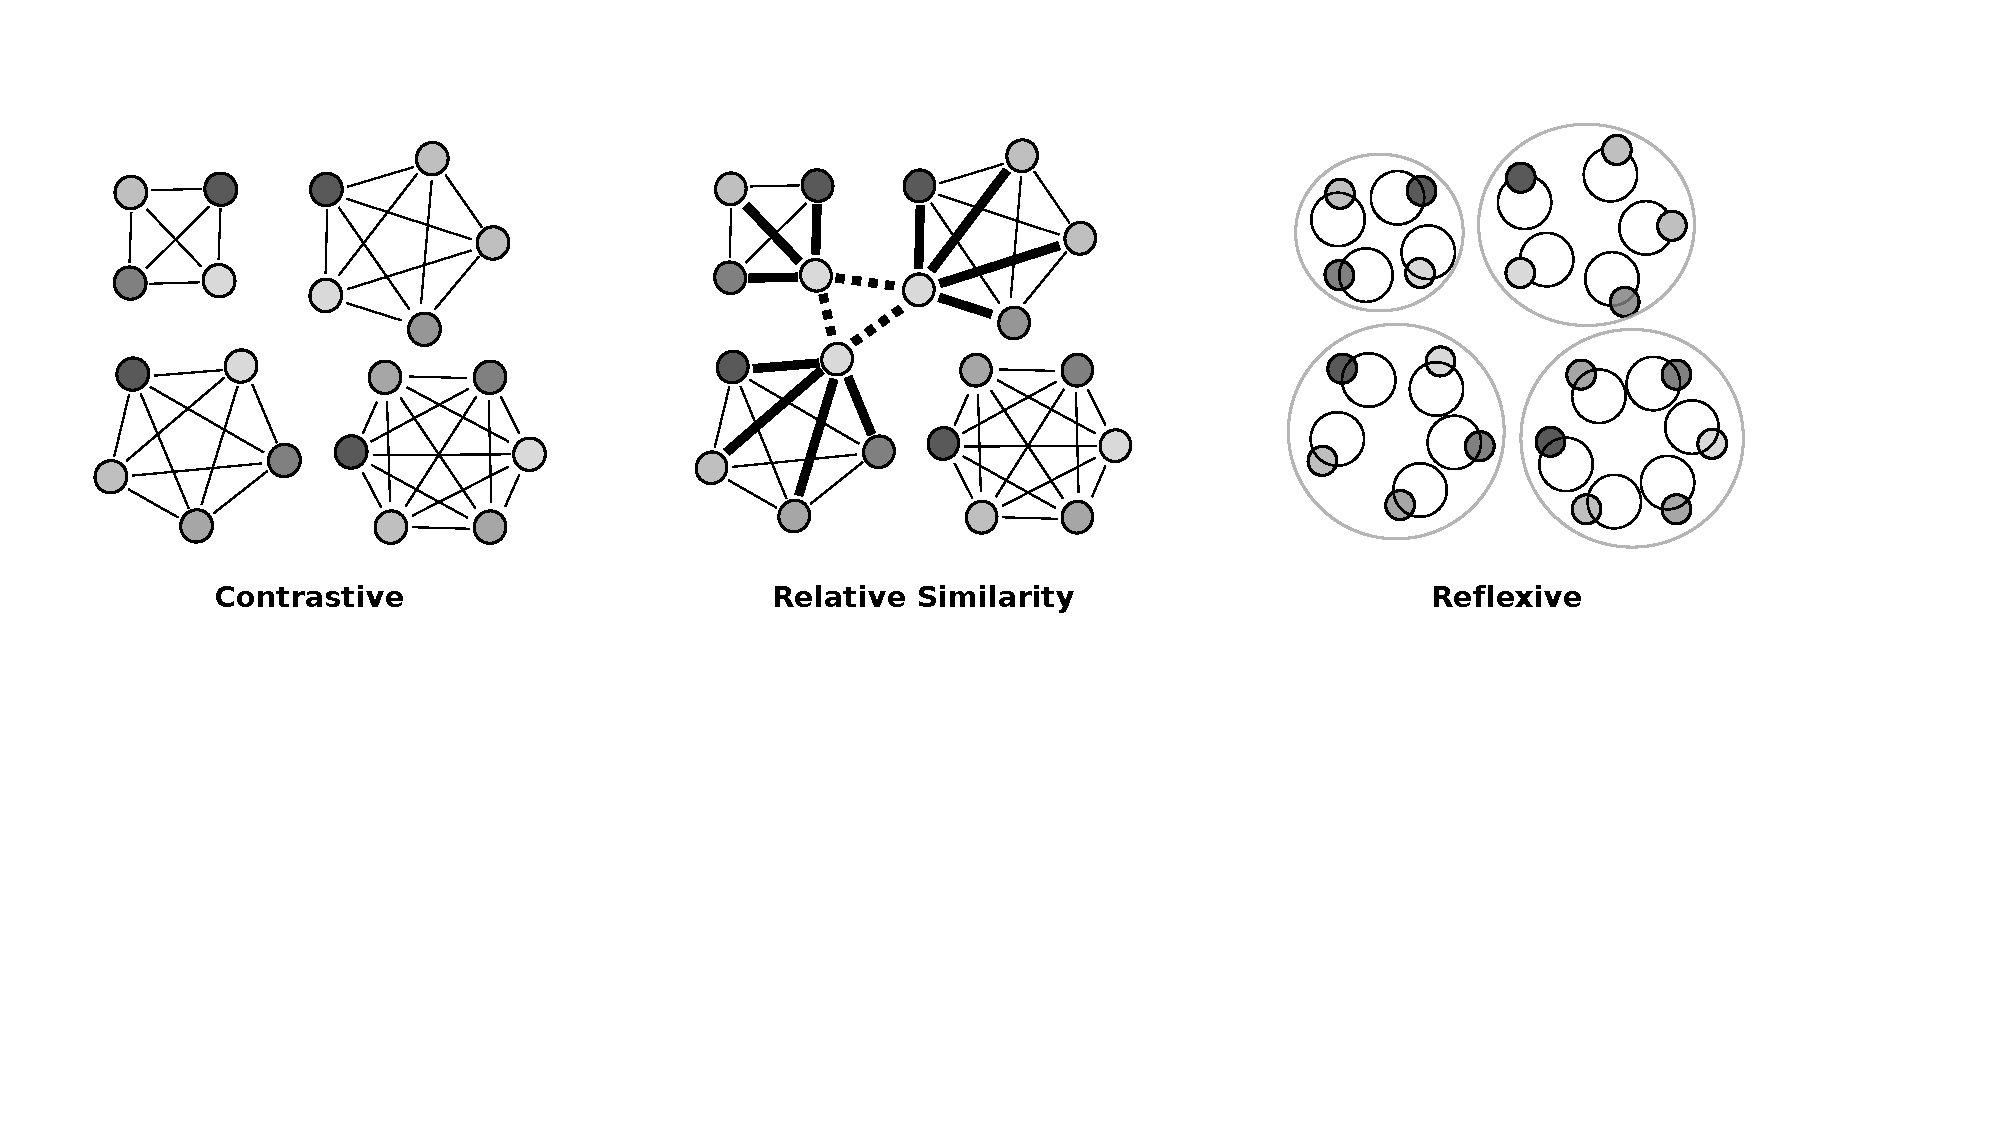
\includegraphics[width=\columnwidth
%     % clip, viewport= 0in 2.65in 12.5in 7.25in
%     ]{figures/Relation}
%         \caption{\small \label{fig:relation} Contrastive, Similarity by contrast and Reflexive strategies among $(q,a)$ tuples. Contrastive strategy is used to compare between all answers to a question;  Similarity by contrast connects answers by the same author across questions if relative difference in author's skill with other answerers in each question are significant. Reflexive assumes no dependence on other answers for prediction. }
%     \vspace{-0.1in}
% \end{figure}
\begin{figure*}[h]
    \centering
    \begin{subfigure}{0.25\textwidth}
        \centering
        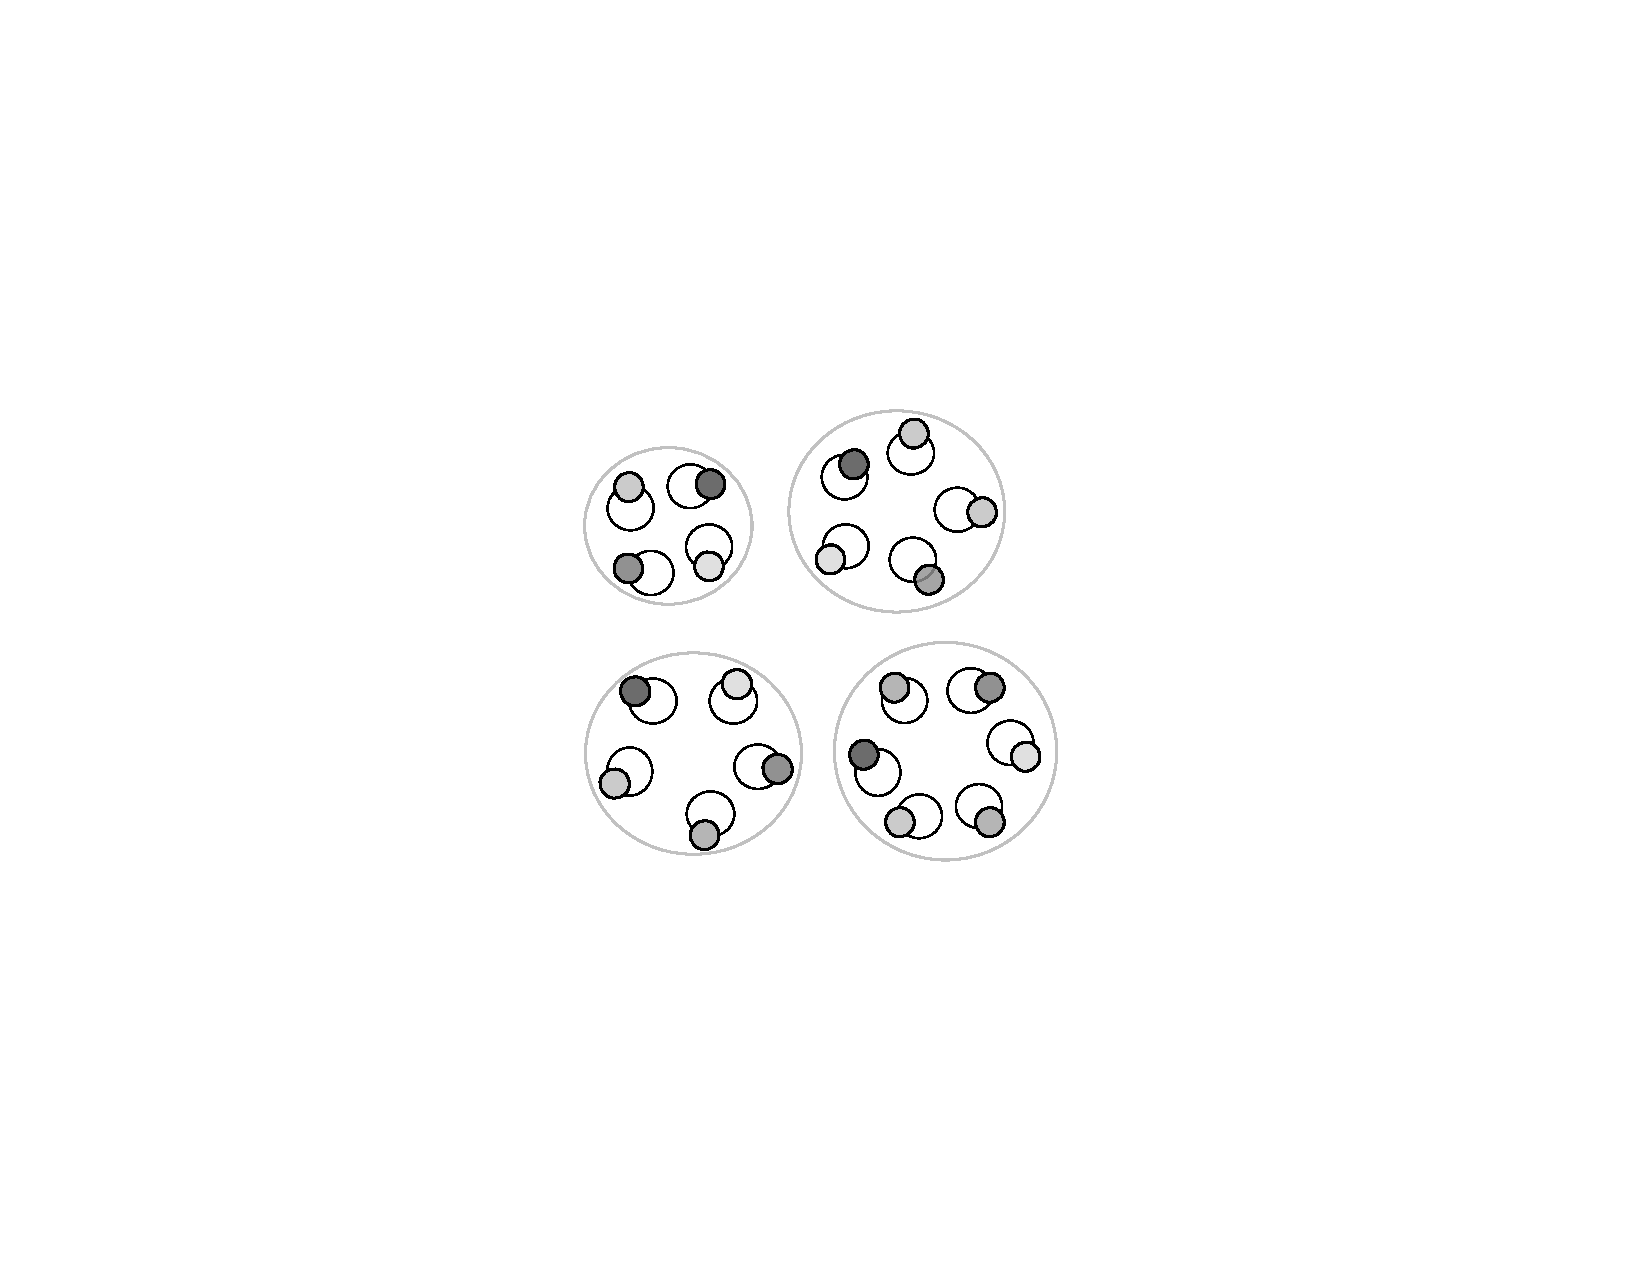
\includegraphics[scale=0.3]{figures/reflex_updated}
            \caption{Reflexive}
            \label{fig:reflexive}
    \end{subfigure}%
    \begin{subfigure}{0.27\textwidth}
        \centering
        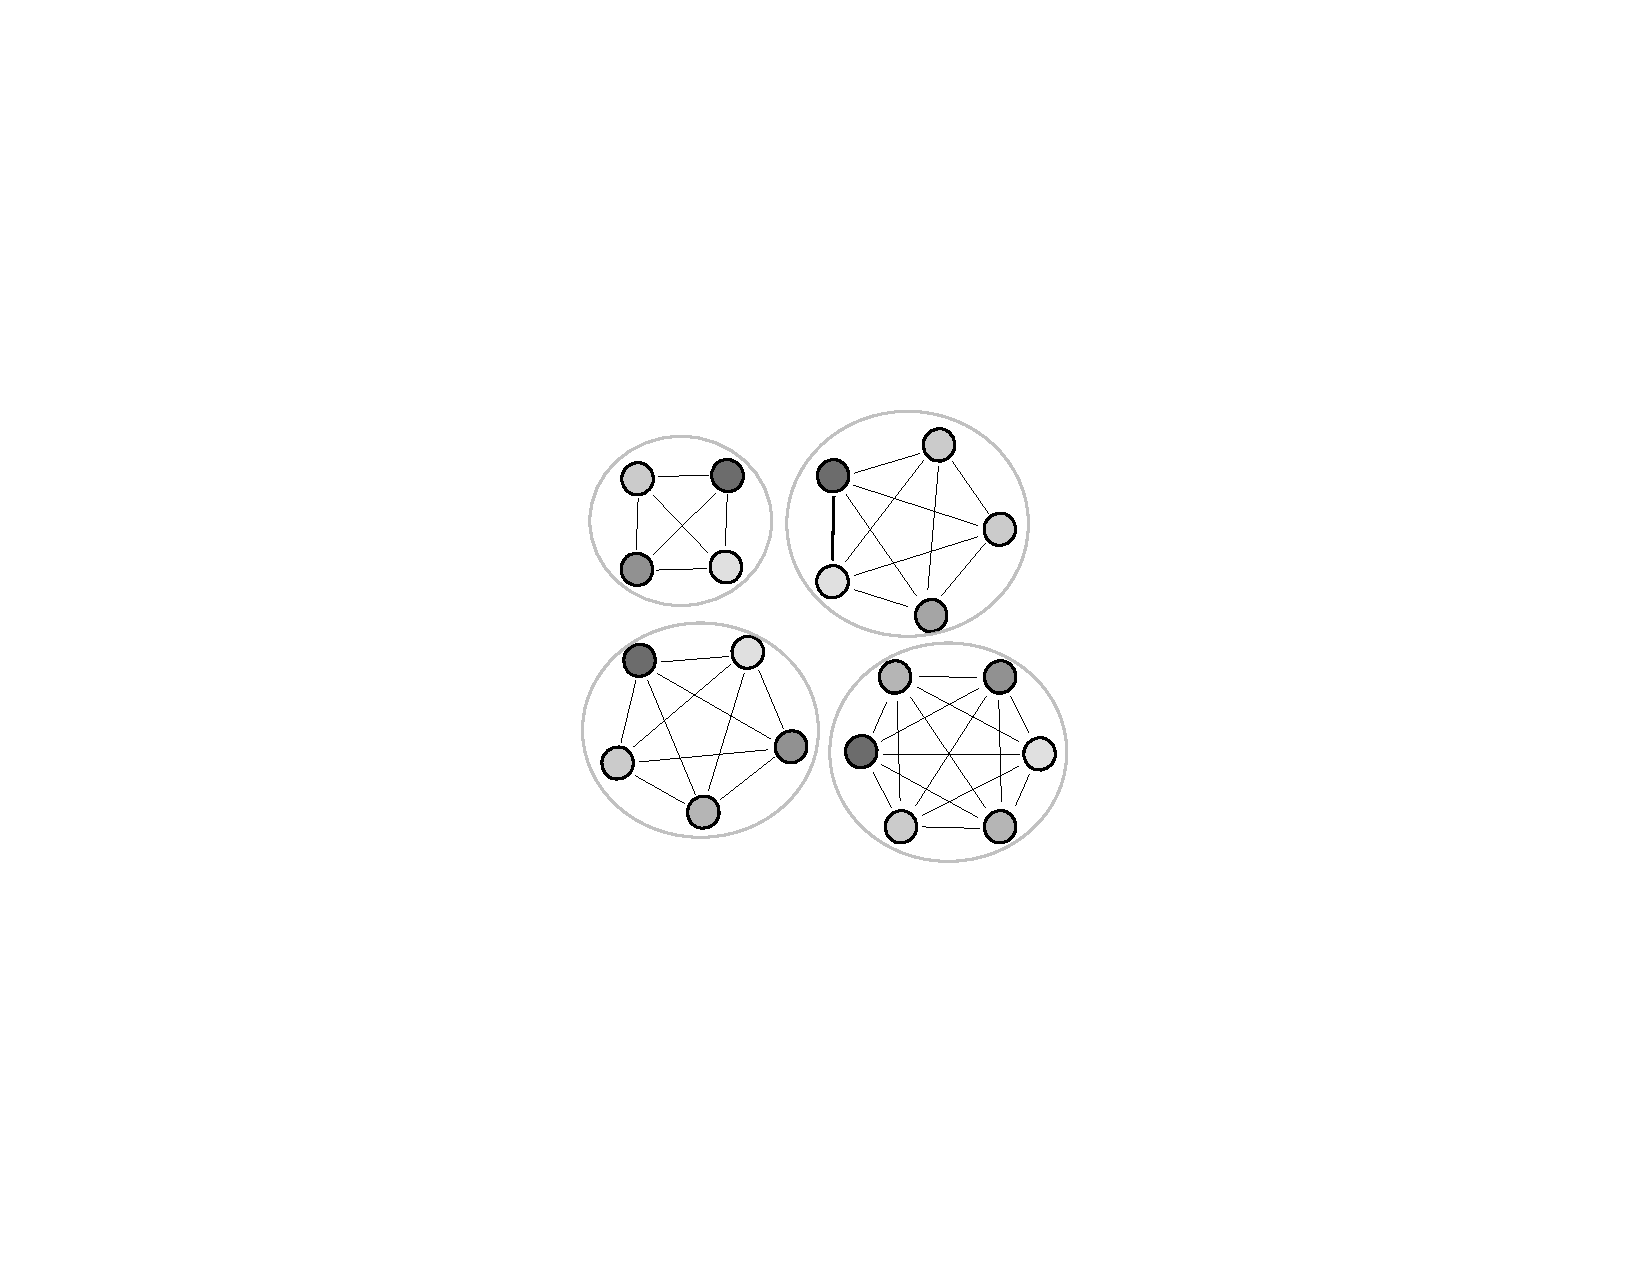
\includegraphics[scale=0.3]{figures/Contrast_circle}
        \caption{Contrastive}
        \label{fig:contrastive}
    \end{subfigure}%
    \begin{subfigure}{0.25\textwidth}
        \centering
        %\includegraphics[width=\linewidth,height=5cm]{figures/drawing}
            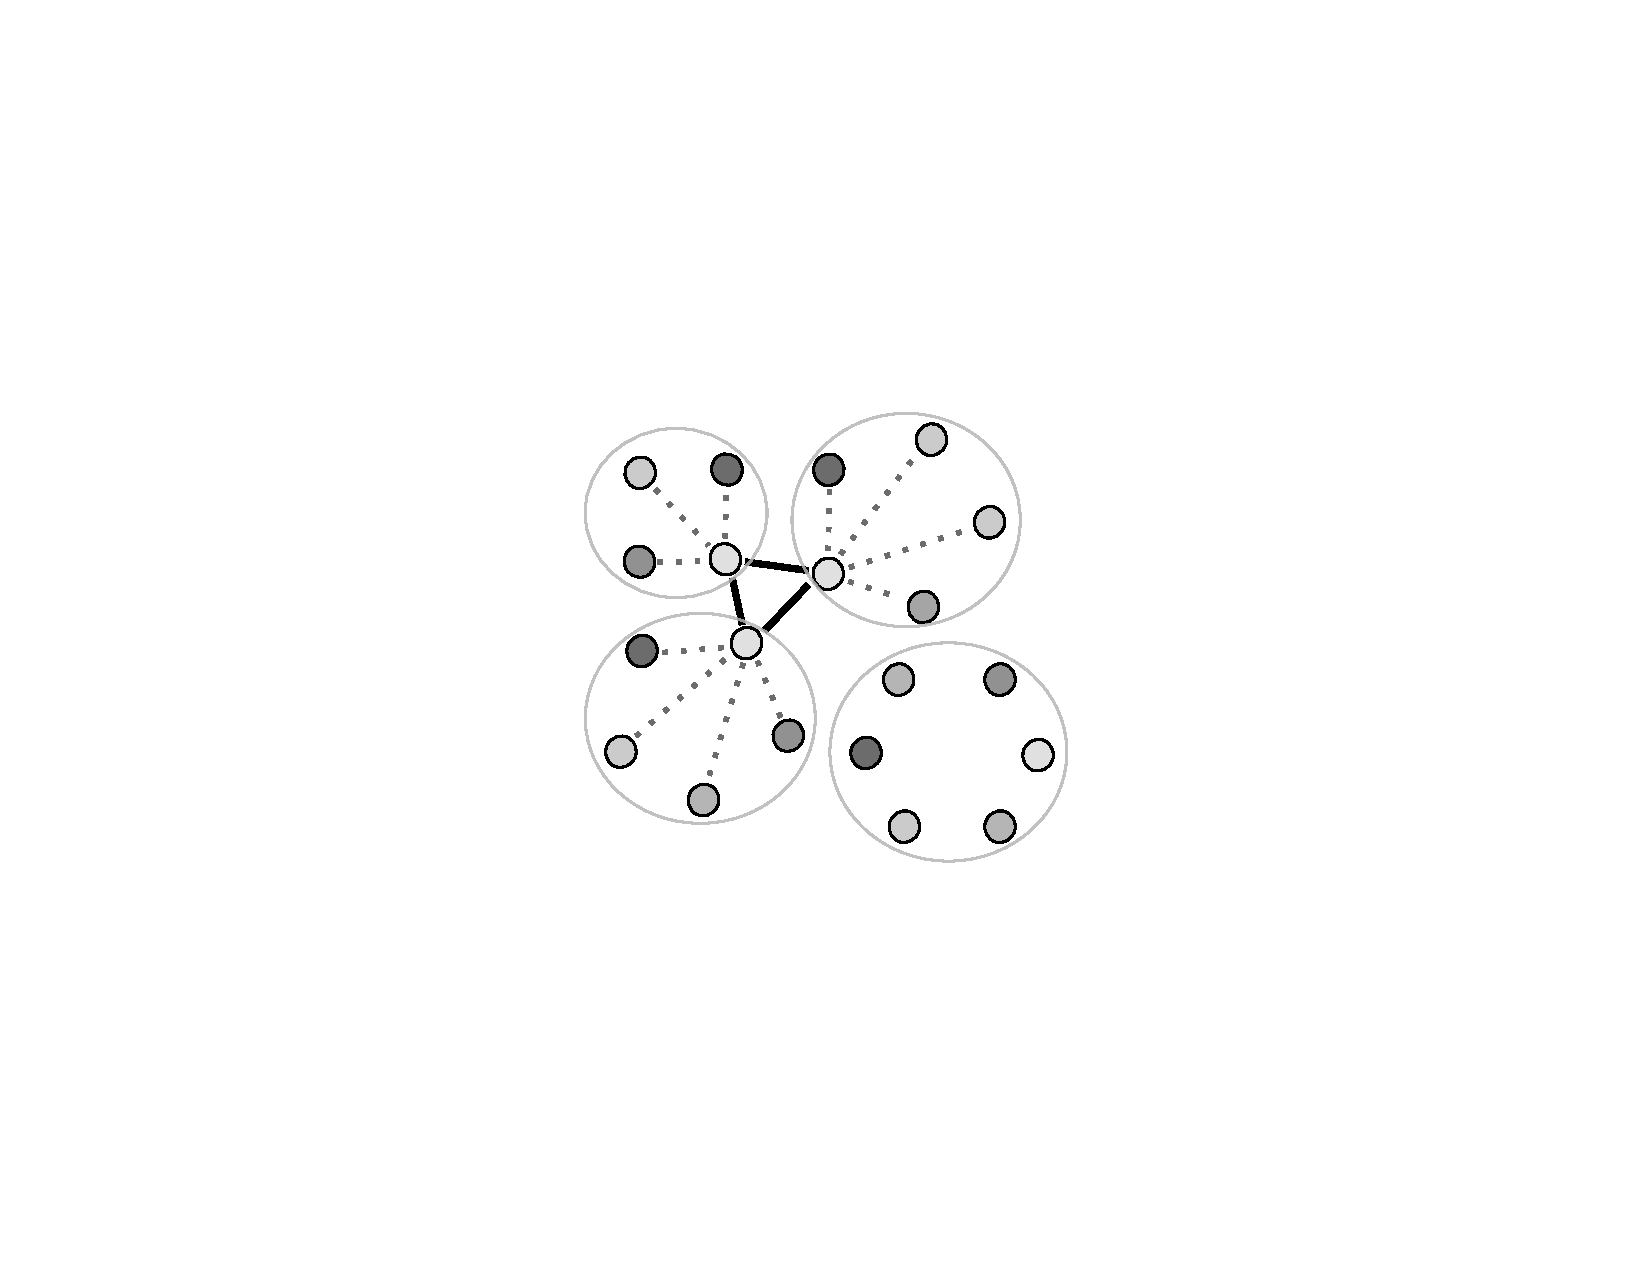
\includegraphics[scale=0.3]{figures/similarContrast_old}
      \caption{Similarity by Contrast}
      \label{fig:similar}
        \end{subfigure}%
        % \begin{subfigure}{0.45\linewidth}
        %     \centering
        %     %\includegraphics[width=\linewidth,height=5cm]{figures/drawing}
        %     \includegraphics[scale=0.275]{figures/Similarity2}
        % \end{subfigure}
        % \caption{TrueSkill / Arrival Similarity}
    %\end{subfigure}%
  %      \caption{\small \label{fig:relation} Induced data-driven relational classes; Contrastive, Relative Similarity and Reflexive among $(q,a)$ tuples. Contrastive relation exists between all answers to a question; Relative Similarity connects answers across questions if relative difference in author's skill with other answerers in each question are significant. Reflexive assumes no dependence on other answers for prediction. }
    \caption{\small \label{fig:relation} Reflexive(~\cref{fig:reflexive}), Contrastive (~\cref{fig:contrastive}) and Similarity by Contrast (~\cref{fig:similar}) relations among $(q,a)$ tuples. Reflexive assumes no dependence on other answers for prediction. Contrastive compares all answers to a question;  Similarity by Contrast connects answers across questions if they differ from other answers similarly. Solid lines indicate similarity, while dotted lines indicate contrast. The contrast is only significant in three questions in the above example.}
    \vspace{-0.15in}
\end{figure*}

%In this section, we define and operationalize the three class of \emph{induced relational views} among the $(q, a)$ tuples introduced above. Each $(q,a)$ tuple constitutes a node in each induced relational view of the dataset. We now describe the precise construction of the links in each view. We aim to facilitate feature sharing (with similarity views) and feature discrimination (with contrastive views) among linked nodes.

%In this section, we define and operationalize the  %Each $(q,a)$ tuple constitutes a node in each induced relational graph of the dataset.
% In this section, we describe the construction of the views representing three different strategies. %We induce these relational views across $(q,a)$ tuples with differing criteria (hence \textit{induced relational views}).

% Our views are designed to achieve feature sharing for the \emph{relative similarity} strategy, feature comparison for the \emph{contrastive} strategy and feature evaluation for the \emph{reflexive} strategy.

%As we observed in the previous section, we formulate answer selection as a node classification problem to facilitate explicit feature sharing (in case of similarity views) and feature discrimination (in case of contrast views) across nodes based on the induced links in each view.

% \begin{wrapfigure}{R}{0.15\textwidth}
% \centering
% \includegraphics[height=3cm,width=0.1\textwidth]{figures/example_human}
% \caption{\small \label{fig:contrast}Contrastive Relation}
% \end{wrapfigure}

%
% \begin{figure}[h]
%     \centering
%     %\includegraphics[height=4cm,width=0.45\textwidth]{figures/clique_size_distribution}
%     \includegraphics[scale=0.15]{figures/clique_size_distribution}
%     \caption{\small \label{fig:clique_size_dist} Distribution of clique sizes for Contrastive relation (i.e. number of answer per question) in StackExchange communities. It follows a long tail distribution with higher variance across communities for large clique sizes.}
%     %\vspace{-0.1in}
% \end{figure}

\subsection{Constructing Induced Views}
\label{sub:Induced Views}


In this section, we discuss four sample strategies that represent strategies to label an answer as `accepted.' Each strategy $S_i \in \mathbf{S}$ \textit{induces} a graph $G_i = (V, E_i)$ (also referred to as a relational view). In each graph $G_i$, a vertex $v \in V$ represents a tuple $(q,a)$ and an edge $e \in E_i, E_i \subseteq V \times V$ connects two tuples that are related under that strategy or view. Note that each $G_i$ has the same vertex set, while edge sets $E_i$ depend on strategy $S_i$. Each strategy employs one of the three different relation types, reflexive, contrastive, and similarity to connect the tuples. We use one reflexive strategy, one contrastive, and two similarity strategies in our experiments. \Cref{fig:relation} summarizes the three relations. We organize the below discussion by relation type.

%In each case, the vertex set $V$ is the same across the different $G_i$, and the edge sets $E_i$ are strategy dependent.
%Each strategy use three different relations between nodes and their corresponding graphs.
%Now we discuss in detail four example strategies that can be used to identify answers that the individual posting the question will label as `accepted'in CQA forums.
%the construction of a graph $G_i = (V, E_i)$ , corresponding to each of the $i=4$ different strategies.
%class of relational views
% \noindent

\subsubsection{Reflexive}
\label{sub:Reflexive}

A natural strategy is to examine each $(q,a)$ tuple in isolation and then assign a label $y_{q,a} \in \{-1,+1 \}$ corresponding to `not accepted' or `accepted.' In this case, $y_{q,a}$ depends on only the features of $(q,a)$. This is a \textbf{Reflexive} relation, and the corresponding graph $G_r = (V,E_r)$ has a specific structure. In particular, in this graph $G_r$, we have only self-loops, and all edges $e \in E_r$ are of the type $(v,v)$. That is, for each vertex $v \in V$, there are no edges $(v,u)$ to any other vertices $u\neq v \in V$. Much of the prior work on feature driven answer selection~\cite{BurelMA16,JendersKN16,TianZL13,TianL16} adopts this view.

\subsubsection{Contrastive}
\label{sub:Contrastive}

A second strategy is to examine answers \textit{in relation} to other answers to the same question and label one such answer as `accepted.' Thus the second strategy \textit{contrasts} $(q,a)$, with other tuples in  $(q,a'), q \in \mathcal{Q}; a, a' \in \mathcal{A}_q; a'\neq a$. This is a \textbf{Contrastive} relation and the corresponding graph $G_c = (V,E_c)$ has a specific structure. Specifically, we define an edge $e \in E_c$ for all $(q,a)$ tuples for the same question $q \in \mathcal{Q}$. That is, if  $v = (q_1, a_1), u=(q_2, a_2)$, $e=(u, v) \in E_c \iff q_1=q_2$. Intuitively, the contrastive relation induces cliques connecting all answers to the same question. Introducing contrasts between vertices sharpens differences between features, an effect (described in more detail in~\Cref{subsec:contrast}) we term \emph{Discriminative Feature Magnification}. Notice that the contrastive relation is distinct from graphs with signed edges (e.g.,~\cite{signedgcn}). In our framework, the contrast is a \textit{neighborhood} property of a vertex, whereas in~\cite{signedgcn}, the negative sign is a property of an \textit{edge}.


% The \textbf{Contrastive} strategy discriminates the features of accepted answers against their competitors. %We propose a specific operationalization of the contrast view drawing upon the tournament view of each question in the forum.
% %\textbf{Tournament-Style Contrast:}
% Thus, we construct links between tuples $(q, a)$ and $(q, a')$ for questions $q \in Q$ and their answers $\texttt{ }\forall \texttt{ } a,a' \in \mathcal{A}_q$ under this view.
% %For questions $q \in Q$, and their answers $\mathcal{A}_q$, we construct links between tuples $(q, a)$ and $(q, a')  \texttt{ }\forall \texttt{ } a,a' \in \mathcal{A}_q$ resulting in a clique of answers to each question.
% The resulting view is a disconnected collection of cliques of answers to each question with size equal to $\lvert\mathcal{A}_q\rvert$ (~\cref{fig:relation}). Note that in each clique, one answer has an accepted label while the rest do not.
% %(the distribution of clique sizes for StackExchange communities is indicated in \cref{fig:clique_size_dist}).
% % The motive of these induced links is better described in \cref{sec:model} where we discuss Induced Relational Graph Convolution to enable feature sharing across vertices for classification in each induced view.
% The connections across accepted and non-accepted answers to a question enable feature contrast. We design our convolutional model to magnify and encode these differences in \cref{subsec:contrast}, an effect we term \emph{Discriminative Feature Magnification}.
% %The set of cliques can thus be given by $\mathbf{C}_q$ consisting of the links between every $(q,a)$ tuple, where the question is $q$ and $a \in \mathcal{A}_q$.

% %The \textbf{Contrastive} view is induced between all competing players in a specific tournament (i.e., competing answers to a question) and captures the disparity between the accepted $(q,a)$ tuples and the rest of the competing answers to a question. The primary objective of contrast  All the $(q, a)$ tuples of a single question is connected to capture feature contrast through an effect we call \textbf{Discriminative Magnification}. We describe this effect in greater detail in the section Our operationalization of the view is as follows:


\subsubsection{Similarity by Contrast}
\label{sub:Similar}
A third strategy is to identify \textit{similar} $(q,a)$ tuples \textit{across} questions. Prior work~\cite{Wu2016} indicates that individuals on StackExchange use diverse strategies to contribute answers. Experts (with a high reputation) tend to answer harder questions, while new members (with low reputation)  looking to acquire reputation tend to be the first to answer a question.

How might similarity by contrast work? Consider two individuals Alice and Bob with \textit{similar} reputations (either high or low) on StackExchange, who contribute answers $a_A$ and $a_B$ to questions $q_1$ and $q_2$ respectively. If Alice and Bob have high reputation difference with other individuals who answer questions $q_1$ and $q_2$ respectively, then it is likely that $(q_1, a_A)$ and $(q_2, a_B)$ will share the same label (if they are both experts, their answers might be accepted, if they are both novices, then this is less likely). However, if Alice has a high reputation difference with other peers who answer $q_1$, \textit{but Bob does not have that difference} with peers who answer $q_2$, then it is less likely that the tuples $(q_1, a_A)$ and $(q_2, a_B)$ will share the label, even though the reputations of Alice and Bob are similar.

Thus the key idea of the \textbf{Similarity by Contrast} relation is that link tuples that are  \textit{similar in how they differ} with other tuples. We construct the graph $G_s = (V, E_s)$ in the following manner. An edge $e = (v,u)$ between tuples $v$ and $u$ exists if the similarity $s(v,u)$ between tuples $v,u$ exceeds a threshold $\delta$. We define the similarity function $s(\cdot , \cdot)$ to encode similarity by contrast. That is, $e=(v,u) \in E_s \iff s(v,u) \geq \delta$.

% \begin{figure}[htbp]
%   \centering
%   \begin{subfigure}{0.23\textwidth}
%     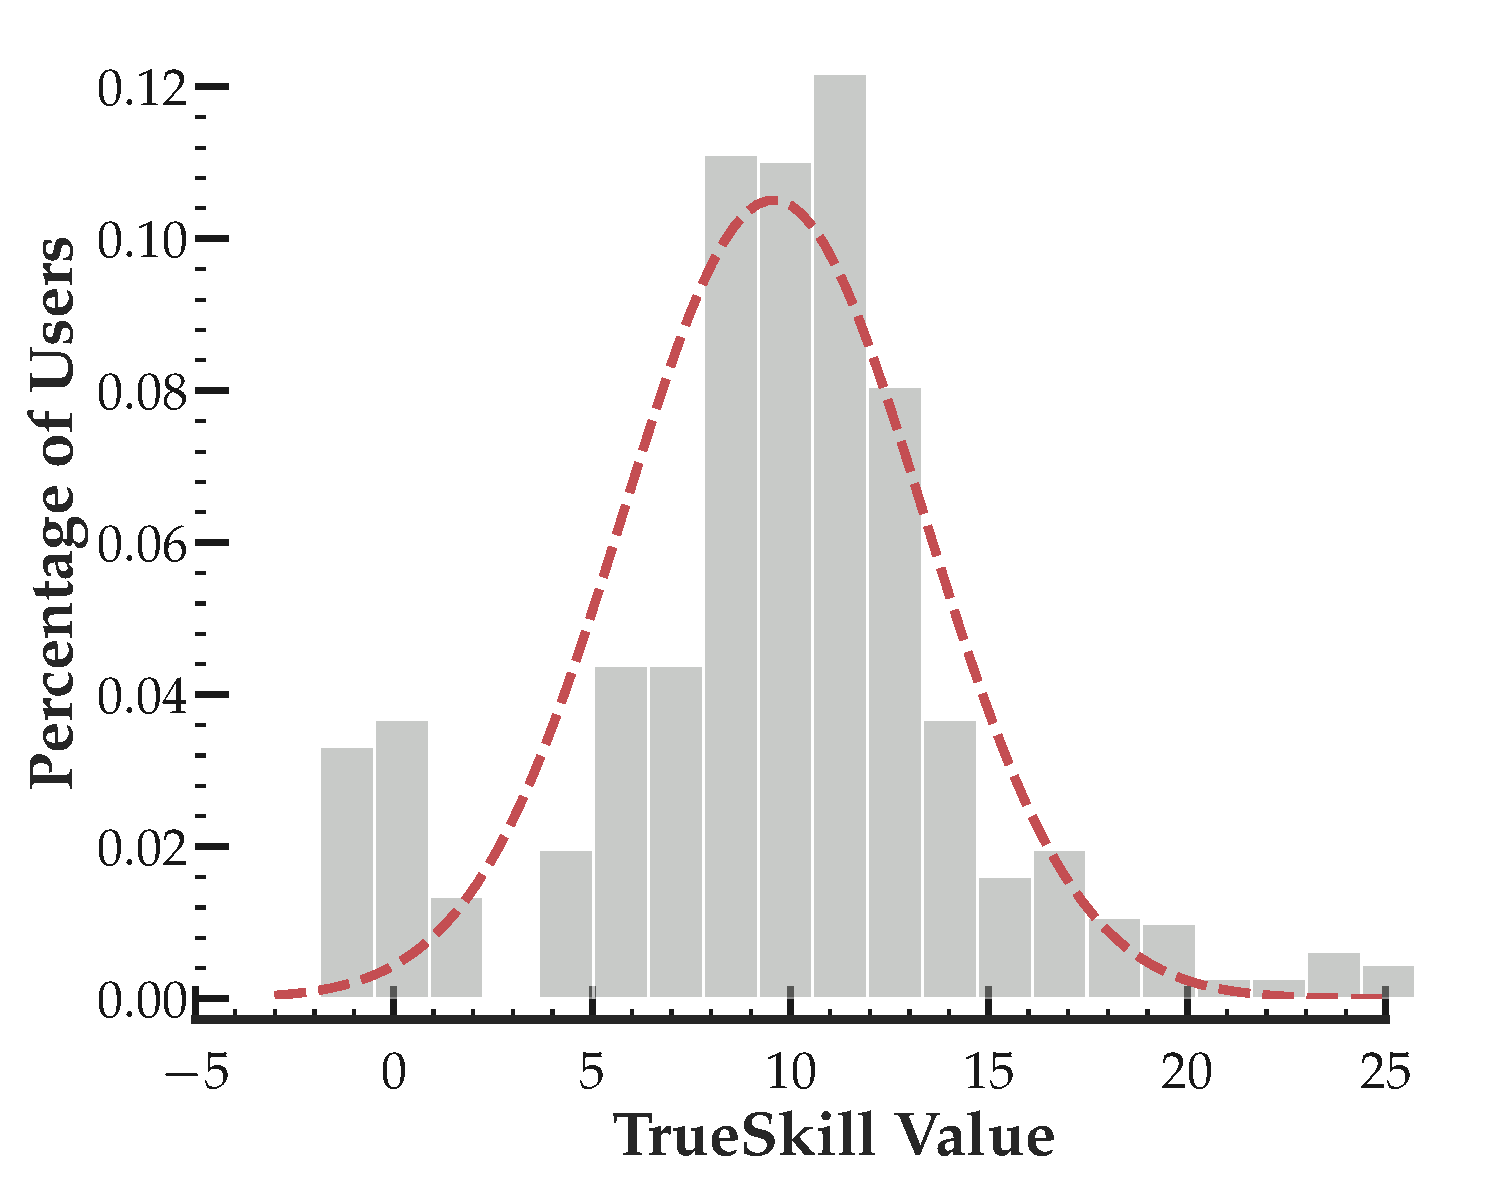
\includegraphics[height=3cm,width=\textwidth]{figures/TrueSkill}
%     \caption{TrueSkill Distribution}
%   \end{subfigure}%
%   \begin{subfigure}{0.23\textwidth}
%     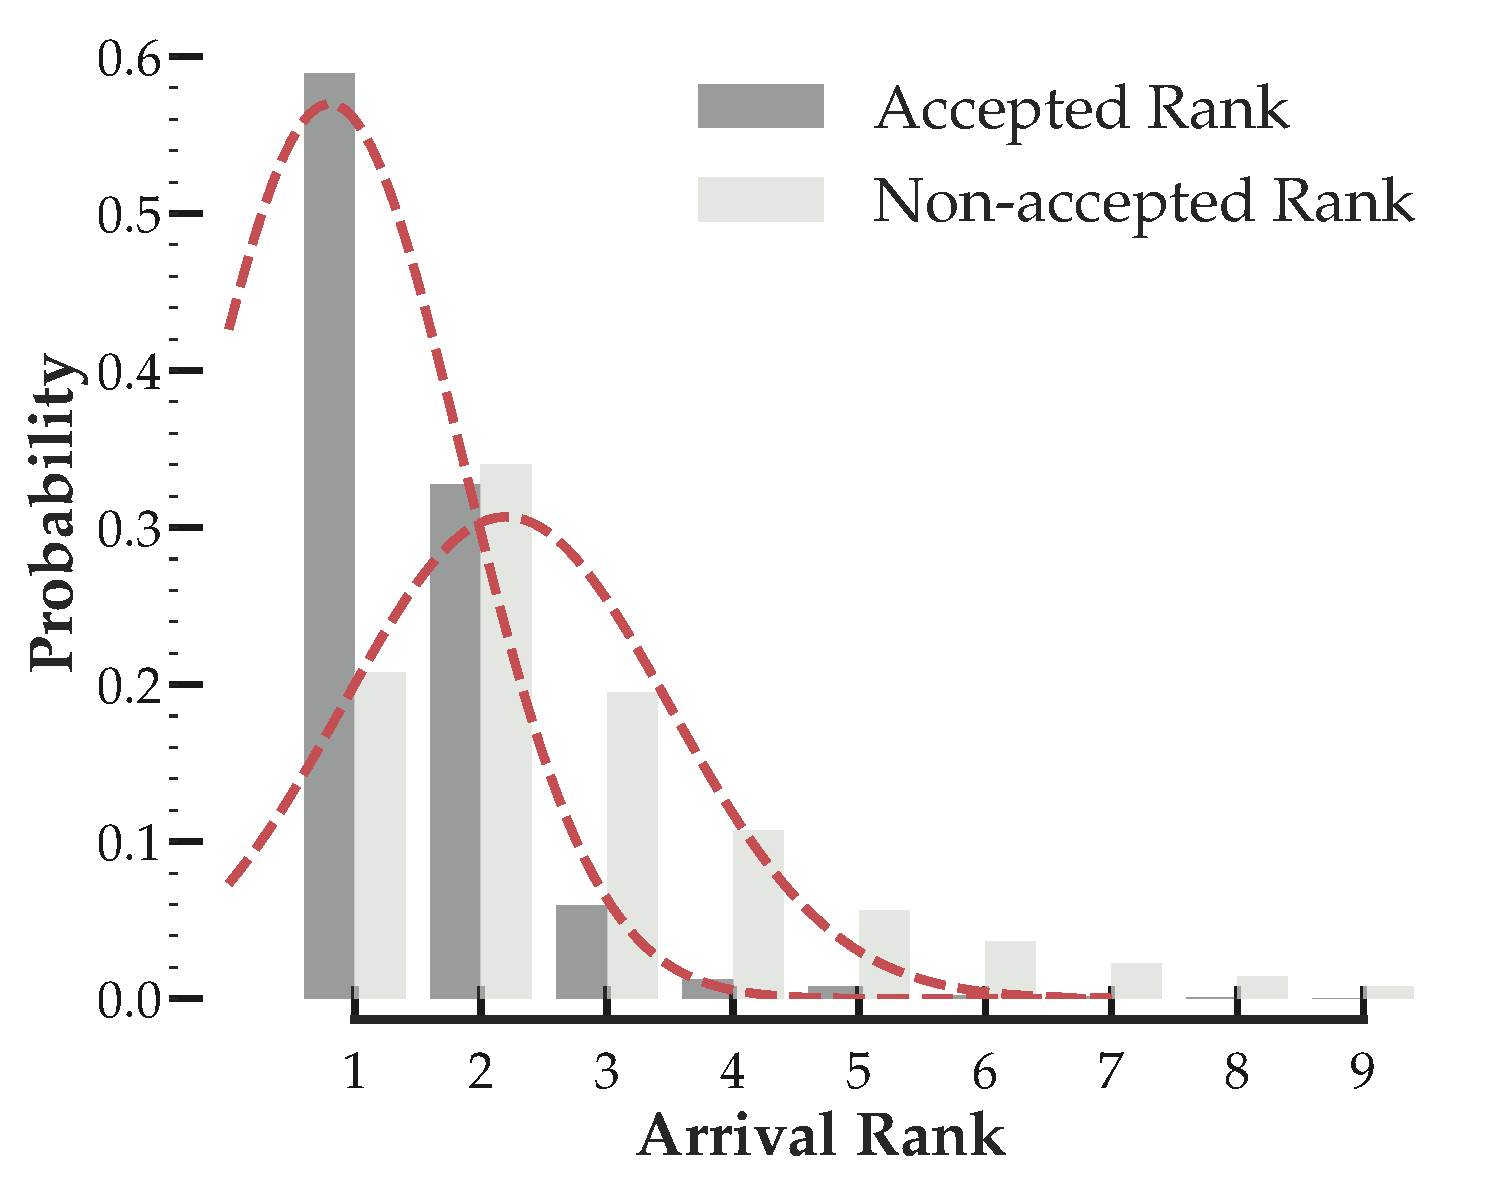
\includegraphics[height=3cm,width=\textwidth]{figures/ArrivalRank}
%     \caption{ArrivalRank Distribution}
%   \end{subfigure}
%   \caption{\small \label{fig:similarcontrastsempirical} Distribution of the TrueSkill values of users and ArrivalRank of accepted answers and non-accepted answers for the movie StackExchange. Early answers are more likely to be accepted and variance of TrueSkill similarity across users is high.}
% \end{figure}

Motivated by~\cite{Wu2016}, we consider two different views that correspond to the similar contrast relation. The \textbf{TrueSkill Similarity} view connects all answers authored by a user where her skill (computed via Bayesian TrueSkill~\cite{TrueSkill06})) differs from competitors by margin $\delta$. We capture both cases when the user is less or more skilled than her competitors. In the \textbf{Arrival Similarity} view, we connect answers across questions based on the similarity in the relative time of their arrival (posting timestamp).
% ~\Cref{fig:similarcontrastsempirical} shows the distribution of skill and the relationship of answer acceptance to arrival rank in StackExchange. We see a wide skill distribution and that the earlier answer has a higher probability of acceptance.
Notice that two Similarity by Contrast views have different edge ($E$) sets since the corresponding similarity functions are different. Notice also, that the two similarity function definitions are transitive.
%%%%%%%INCLUDE COAUTHOR REASON
 \footnote{One trivial way of establishing similarity is co-authorship i.e. connect all $(q,a)$ tuples of a user (probably on the same topic) across different questions.
%Thus, we can connect each $(q,a)$ and $(q',a'); q,q' \in \mathcal{Q}, a \in \mathcal{A}_q, a' \in \mathcal{A}_q'$ such that $u_a = u_{a'}$.
Note that the accepted answer is labeled relative to the other answers. As the competing answers are different in each question, we can not trivially assume acceptance label similarity for all co-authored answers. In our experiments, co-authorship introduced a lot of noisy links in the graph leading to worse performance.}

\subsection{Generalized Views}
\label{sub:Generalized Views}
Now we present the general case of the induced view. First, notice that each of the three relation types that we consider---reflexive, contrastive, and similarity---result in a graph $G_i = (V, E_i)$ comprising a set of cliques. This is not surprising, since all three relations presented here, are equivalence relations. Second, observe the semantics of how we select the tuple with the accepted answer. Within the three relations, we used two semantically different ways to assign the `accepted' answer label to a tuple. One way is to share the labels amongst all the vertices in the \textit{same clique} (used in the reflexive and the similarity relations). The second is to \textit{assign label based on contrasts with other vertices} in the same clique. We can now state the organizing principle of our approach as follows.
\begin{quote}
  A generalized \textit{modular} framework: pick a meaningful equivalence relation on the $(q,a)$ tuples to induce graph comprising cliques and then apply specific label semantics (label sharing or label contrast) within each clique.
\end{quote}

Equivalence relation results in a graph with a set of disconnected cliques. %Then, within a clique, one could use application-specific semantics, different from two discussed in this paper, to label tuples as `accepted.'
%For example, we could restrict the determination of label via contrast to tuples that satisfy some criteria (e.g., gender, location, education, etc.).
Cliques have some advantages: they have well-defined graph spectra~\cite[p. 6]{Chung1997}; cliques allow for \textit{exact} graph convolution; parallelize the training as the convolution of a clique is independent of other cliques.
%parallelize training and testing.

%Thus, each strategy induces a graph $G_i=(V,E_i)$ using one of the three equivalence relations---reflexive, contrastive, and similarity---and then applies one of the two semantics (`share the same label'; `determine label based on contrast').
% While the modular separation between graph construction and label semantics does not imply that we construct the graph (or the view) $G$ via an equivalence relations,


% Cliques have well defined graph spectra~\cite{Chung1997} and may speed up Graph Convolution Networks (GCNs) by running the convolution in parallel across cliques.

% Thus, our induced view framework readily generalizes to admit \textit{any} equivalence relation. Equivalence partitions of vertices in $G$ result in cliques. Then, within a clique, one could use application specific semantics to label tuples as `accepted.' For example, we could also consider alternate semantics such as `label at most two answers as `accepted'' etc. Cliques have well defined graph spectra~\cite{Chung1997} and may potentially speed up Graph Convolution Networks (GCNs) by running the convolution in parallel across cliques.




% we next discuss induced relational GCNs.

% and then applies a specific semantic (`contrast'; `similar').

%Thus far, we've discussed $i=4$ strategies, and their corresponding views or graphs $G_i = (V, E_i)$. Each strategy used one of the three equivalence relations---reflexive, contrast, similar---resulting in $G_i$ being a set of cliques. We introduced two label selection mechanisms (`share labels within a clique', `assign label by contrast'), and in the next section we show how to make operational these mechanisms on a view $G_i$ via a graph convolution.
% equivalence relations---reflexive, contrastive and similar---and the corresponding graphs $G_k = (V,E_k)$ along with two different

% provides a temporal metric against competitors. The temporal arrival patterns of answers are correlated to their acceptance probabilities (\cref{fig:clique}). For a specific user authoring answers $a, a'$ to questions $q, q'$, we establish a link between $(q,a)$ and $(q',a')$ if %$\lvert T_{a} - T_{b} \rvert > \gamma \times \max(T_{b}); \forall b \in \mathcal{A}_(q)$ and $\lvert T_{a'} - T_{c} \rvert > \gamma \times \max(T_{c}); \forall c \in \mathcal{A}_(q')$.
% %Highly skilled/active users tend to follow consistent patterns in when they author answers, relative to the other competing answers.
% %We observe that earlier posted answers have a higher chance of acceptance in CQA platform as shown in Figure \ref{fig:clique}. Therefore,
% \begin{align*}
%  \lvert T_{a} - T_{b} \rvert &> \gamma \times \max(T_{b}), \hspace{3pt} \forall b \in \mathcal{A}_(q), b \neq a \hspace{5pt} \textsc{AND} \\
%  \lvert T_{a'} - T_{c} \rvert &> \gamma \times \max(T_{c}), \hspace{3pt} \forall c \in \mathcal{A}_(q'), c \neq a'
% \end{align*}
% where $T_{a}$ represents the number of seconds between the question and answer $a$. Hence we connect answers that are quicker or slower than their competitors by a $\gamma$ factor.


% Specifically, if the user authors answers $a, a'$ to questions $q, q'$, we connect tuples $(q,a)$ and $(q',a')$ where %$\lvert S_{u_a} - S_{u_b} \rvert > \delta; \forall b \in \mathcal{A}_(q)$ and $\lvert S_{u_a'} - S_{u_c} \rvert > \delta; \forall c \in \mathcal{A}_(q')$
% \begin{align*}
%  \lvert \textit{TS}_{u_a} - \textit{TS}_{u_b} \rvert &> \delta, \hspace{3pt} \forall b \in \mathcal{A}_(q), b \neq a  \hspace{5pt} \textsc{AND}\\
%  \lvert \textit{TS}_{u_{a'}} - \textit{TS}_{u_c} \rvert &> \delta, \hspace{3pt} \forall c \in \mathcal{A}_(q'), c \neq a'
% \end{align*}
% where $\textit{TS}_{u_a}$ is the skill value for the user who authored answer $a$ (we estimate user skill values with TrueSkill rating \cite{TrueSkill06}). This captures both cases, i.e. where the user is less or more skilled than his competitors.







% For example, answers by individuals with low reputation are likely not `accepted' for a question if there is also an answer by an individual with high reputation to the same question. Thus two tuples $(q,a), q \in \mathcal{Q}, a \in \mathcal{A}_q$ and $(q',a'), q' \in \mathcal{Q}, a \in \mathcal{A}_{q'}$ by (possibly different) low-reputation individuals are \textit{similar in how they differ} with other tuples corresponding to the same questions $q$ and $q'$ respectively.


% \textbf{Reflexive} strategy evaluate $(q, a)$ tuples in isolation as illustrated in \cref{fig:relation}. In such cases, the label prediction for $(q, a)$ tuple depends on it's features alone. This view encompasses most feature-driven answer selection methodology~\cite{BurelMA16,  JendersKN16, TianZL13, TianL16}.





% \noindent
% The \textbf{Similarity} \emph{by contrast} strategy connects answers across different questions by relative comparison against their competitors. Consider a simplified example (~\cref{fig:relation}); user Alice answers four questions with varying numbers of competing answers. Assume a wide skill-margin between Alice and the authors of the other answers in three questions. In these three cases, it is likely that her answer is accepted or the converse depending on her relative skill. However, results are uncertain in scenarios where the author skill differences are not as pronounced. The relative similarity of Alice's answers (high skill margins) to competing answers enables us to make a confident prediction. Hence, one way to create a \emph{similarity by contrast} view is by author skill. We create two diverse similarity by contrast views in our experiments:%In a more general sense, this is true of other answer features as well.

%Therefore, tournament outcomes are likely to be similar when answers are authored by users who differ from those of competing answers by significant margins. There are two such cases, the user has a significantly greater skill than the competing authors, and the opposite case. The intermediate cases are more uncertain. The resulting graph is again a complete graph as all such $(q, a)$ pairs are connected to each other.

 %By employing author skill as a proxy, we are able to learn the associations of other answer features to the acceptance outcome.


% The \textbf{TrueSkill Similarity} view connects all the answers authored by a user where his skill differs from competitors by margin $\delta$. Specifically, if the user authors answers $a, a'$ to questions $q, q'$, we connect tuples $(q,a)$ and $(q',a')$ where %$\lvert S_{u_a} - S_{u_b} \rvert > \delta; \forall b \in \mathcal{A}_(q)$ and $\lvert S_{u_a'} - S_{u_c} \rvert > \delta; \forall c \in \mathcal{A}_(q')$
% \begin{align*}
%  \lvert \textit{TS}_{u_a} - \textit{TS}_{u_b} \rvert &> \delta, \hspace{3pt} \forall b \in \mathcal{A}_(q), b \neq a  \hspace{5pt} \textsc{AND}\\
%  \lvert \textit{TS}_{u_{a'}} - \textit{TS}_{u_c} \rvert &> \delta, \hspace{3pt} \forall c \in \mathcal{A}_(q'), c \neq a'
% \end{align*}
% where $\textit{TS}_{u_a}$ is the skill value for the user who authored answer $a$ (we estimate user skill values with TrueSkill rating \cite{TrueSkill06}). This captures both cases, i.e. where the user is less or more skilled than his competitors.
%\begin{align*}
% \lvert S_{u,a} - S_{u, b} \rvert < -\delta; \forall b \in \mathcal{A}(q) \\
% \lvert S_{u,a'} - S_{u, c} \rvert < -\delta; \forall c \in \mathcal{A}(q')
%\end{align*}
%TrueSkill values are normally distributed among users (\cref{fig:clique}).

% developed by Microsoft Reasearch for ranking and matching similar skill game players for Xbox Live. In our settings, each question is a multi player game with all answerers as game players. The user who gives credible answer is the winner. True Skill rating then computes player's skill through bayesian inference on the basis of credibility label of his answered questions. The estimated ratings are a Gaussian distribution where $\mu$ denotes the average skill of the player. We use the mean value as skill value for our computations.

%Therefore, each user can have at most two cliques, one which connects all his answers where his true skill is significantly better than other answerers of the question; and second where his skill is vastly lower than all the other answerers. In the first case, he is highly likely to give accepted answers while in other his answer would be classified as non-accepted. As CQA platforms encompass variety of topics, each user can be accepted in one topic while non accepted for other topics in the same community.

% Formally, output of the $i$-th hidden layer for True Skill Similarity GCN network $Z_{ts}^{(k)}$ is defined as:
% \begin{equation}
%   \label{eq:TSsimilarity}
%   Z_{ts}^{k} = \sigma\left((I_N + D^{-\frac{1}{2}}A_{ts}D^{\frac{1}{2}}) Z_{ts}^{(k-1)}W_s^{(k)} \right)
% \end{equation}
% with $A_{ts}$ being the adjacency matrix for true skill similarity relations.


% \textbf{Arrival Similarity} view provides a temporal metric against competitors. The temporal arrival patterns of answers are correlated to their acceptance probabilities (\cref{fig:clique}). For a specific user authoring answers $a, a'$ to questions $q, q'$, we establish a link between $(q,a)$ and $(q',a')$ if %$\lvert T_{a} - T_{b} \rvert > \gamma \times \max(T_{b}); \forall b \in \mathcal{A}_(q)$ and $\lvert T_{a'} - T_{c} \rvert > \gamma \times \max(T_{c}); \forall c \in \mathcal{A}_(q')$.
% %Highly skilled/active users tend to follow consistent patterns in when they author answers, relative to the other competing answers.
% %We observe that earlier posted answers have a higher chance of acceptance in CQA platform as shown in Figure \ref{fig:clique}. Therefore,
% \begin{align*}
%  \lvert T_{a} - T_{b} \rvert &> \gamma \times \max(T_{b}), \hspace{3pt} \forall b \in \mathcal{A}_(q), b \neq a \hspace{5pt} \textsc{AND} \\
%  \lvert T_{a'} - T_{c} \rvert &> \gamma \times \max(T_{c}), \hspace{3pt} \forall c \in \mathcal{A}_(q'), c \neq a'
% \end{align*}
% where $T_{a}$ represents the number of seconds between the question and answer $a$. Hence we connect answers that are quicker or slower than their competitors by a $\gamma$ factor.
%\begin{align*}
% \lvert T_{a} - T_{b} \rvert < -\gamma * max(T_{b}); \forall b \in \mathcal{A}(q) \\
% \lvert T_{a'} - T_{c} \rvert < -\gamma * max(T_{c}); \forall c \in \mathcal{A}(q')
%\end{align*}
% Our hypothesis is that a similar answering schedule is correlated with acceptance probabilities.

%\begin{comment}
%is based on similarity in the difference of arrival time of answers for a question.
%Consider this hypothetical example, for $q$, the timestamp(minutes) of the difference in answers' arrivals with respect to question's post timestamp are listed below:\\
%$a_1$: 10 \\
%$a_2$: 10000 \\
%$a_3$: 10100 \\
%$a_4$: 10110 \\
%There is higher likelihood of $a_1$ being judged the credible answer as it occured 10 minutes of posting the question. CQA platforms are used for quick discussions and answers posted much later, although could be correct, have much lower likelihood of being accepted. Also note that, for StackExchange, questioner can not change their accepted answer at a later time.
%While for Q2, the timestamp(minutes) of the difference in answers' arrivals to the timestamp of question's posting are:\\
%$a_1$: 10 \\
%$a_2$: 11 \\
%$a_3$: 12 \\
%$a_4$: 1000000 \\
%which means $a_4$ is highly probable not to be accepted.
%\end{comment}

%Thus, for each user, we construct a clique of all answers in which she answers significantly earlier than other answers, and another clique with all answers in which her answer is much later than all other answers for that question.

%
% Formally, output of the $k$-th hidden layer for Arrival Similarity GCN network $Z_{as}^{(k)}$ is defined as:
% \begin{equation}
%   \label{eq:ASsimilarity}
%    Z_{as}^{k} = \sigma \left((I_N + D^{-\frac{1}{2}}A_{as}D^{\frac{1}{2}}) Z_{as}^{(k-1)}W_s^{(k)} \right)
% \end{equation}
% with $A_{as}$ being the adjacency matrix for arrival similarity relationship.




%As noted before, answer selection is a relational property. Thus standard similarity relationships among users of similar skills do not help label prediction. For instance, in the given example, even if Alice has good ratings, she has to be better in \emph{relative} to all other players in the tournament.


% \begin{wrapfigure}{R}{0.15\textwidth}
% \centering
% \includegraphics[height=1.85cm,width=0.1\textwidth]{figures/Reflexive_v2}
% \caption{\small \label{fig:reflex}Reflexive Relation}
% \end{wrapfigure}
%\paragraph{}
%\vspace*{-\parskip}



% Secondly, the tournament-style contrast view is deterministic, we can precisely determine the set of competing answers to a given question (or tournament). On the other hand, relative similarity can be operationalized in many ways (TrueSkill and Arrival Similarity are two relevant views in CQA) and the induced links are inherently noisy. This is a key factor to consider when we develop our node classification architecture in the next section.

%In contrast to Ts. In this paper, we propose an automated graph construction mechanism using data driven induced relationships with minimal human supervision. The graph construction is based on certain user defined criterions which are domain dependent and can be easily adapted to other domains. Note that this is a generic framework and we can introduce other higher-order relationships (like triangles) for different domains.


% Finally, \textbf{Reflexive} strategy evaluate $(q, a)$ tuples in isolation as illustrated in \cref{fig:relation}. In such cases, the label prediction for $(q, a)$ tuple depends on it's features alone. This view encompasses most feature-driven answer selection methodology~\cite{BurelMA16,  JendersKN16, TianZL13, TianL16}.

%This is inherently similar to what current approaches work on. The classification model makes independent prediction and can be representated by a self loop in the graph.
% That is, each node just depends on it's own features and there is no relation to any other node in the graph.
%Knolwedge graphs are widely used in literature \cite{} for understanding graph structured data. Although these graphs support multiple edge types, these edges are manually labeled. Thus, obtaining this edge information can prove to be expensive and restricts scope of these approaches. In this paper, we propose an automated graph construction mechanism using data driven induced relationships with minimal human supervision. The graph construction is based on certain user defined criterions which are domain dependent and can be easily adapted to other domains. Note that this is a generic framework and we can introduce other higher-order relationships (like triangles) for different domains.

%These relationships can be operationalized in different ways and we next explain our interpretation of these relationships for Answer Selection. We further encode these induced relationships using Graph Convolution Networks (GCN).
%\clearpage

\section{Induced Relational GCN}
\label{sec:gcn}
%In this section, we first summarize basic Graph convolution (GCN) model proposed for computing vertex representations in Section \ref{subsec:graph}. We then elaborate upon our operationalization of Contrastive relation in the GCN framework in Section \ref{subsec:contrast}, Similarity relation in Section \ref{subsec:similar} followed by Reflexive relation in Section \ref{subsec:reflex}.
Now, we will encode the two label assignment mechanisms within a clique
%---assign label based on the contrast with clique tuples; share labels amongst tuples in the same clique---
via a graph convolution. First, we briefly review Graph Convolution Networks (GCN) and identify some key concepts. Then, given the views $G_i$ for the four strategies, we show how to introduce label contrasts in~\Cref{subsec:contrast} followed by label sharing in~\Cref{subsec:similar}.
%We refer to the operations on each view as an Induced Relational Graph Convolutional Network (\textbf{IR-GCN}).

%This magnification results in improved separability of classes in the manifold learned by the neural network (further discussion in \cref{ref:analysis}).

\subsection{Graph Convolution}
\label{subsec:graph}
Graph Convolution models adapt the convolution operations on regular grids (like images) to irregular graph-structured data $G = (V,E)$, learning low-dimensional vertex representations. If for example, we associate a scalar with each vertex $v \in V$, where $|V| = N$, then we can describe the convolution operation on a graph by the product of signal $x \in \mathbb{R}^N$ (feature vectors) with a learned filter $g_\theta$ in the fourier domain. Thus,
\begin{equation}
  g_\theta \ast x =  U \, g_\theta \, U^T x,
  \label{eq:basic_gcn}
  % g_\theta (U \Lambda U^T) x =
\end{equation}
where, $\Lambda$ and $U$ are the eigenvalues and eigenvector of the normalized graph Laplacian, $L = I_N - D^{-\sfrac{1}{2}}AD^{\sfrac{1}{2}}$, and where $L = U \Lambda U^T$. $A$ denotes the adjacency matrix of a graph $G$ (associated with a view) with $N$ vertices. ~\Cref{eq:basic_gcn} implies a filter $g_\theta$ with $N$ free parameters, and requires expensive eigenvector decomposition of the adjacency matrix $A$. Deferrard et al.~\cite{deferrard} proposed to approximate $g_\theta$, which in general is a function of $\Lambda$, by a sum of Chebyshev polynomials $T_k(x)$ up to the $k$-th order. Then,

\begin{equation}
  g_\theta \ast x \approx U \, \sum_{k=0}^K \theta_k T_k(\tilde{\Lambda}) \, U^T x \approx \, \sum_{k=0}^K \theta_k T_k(\tilde{L}) \, x,
  \label{eq:approx_gcn}
  % g_\theta (U \Lambda U^T) x =
\end{equation}
where, $\tilde{\Lambda} = 2 \Lambda/ \lambda_{\max}- I_N$ are the scaled eigenvalues and $\tilde{L} = 2L/\lambda_{max} - I_N$ is the corresponding scaled Laplacian. Since $\tilde{L} = U \tilde{\Lambda} U^T$, the two equations are approximately equal.


%The corresponding scaled Laplacian is $\tilde{L} = 2L/\lambda_{max} - I_N$. Since $\tilde{L} = U \tilde{\Lambda} U^T$,~\Cref{eq:approx_gcn} transforms to:
% \begin{equation}
%   g_\theta \ast x \approx \, \sum_{k=0}^K \theta_k T_k(\tilde{L}) \, x.
%   \label{eq:updatedapprox_gcn}
%   % g_\theta (U \Lambda U^T) x =
% \end{equation}

The key result from Deferrard et al.~\cite{deferrard} is that~\Cref{eq:approx_gcn} implies $k$-hop localization---the convolution result depends only on the $k$-hop neighborhood. In other words,~\Cref{eq:approx_gcn}  is a $k$-hop approximation.

However, since we use equivalence relations in our framework that result in cliques, we can do an \textit{exact} convolution operation since vertices in a clique only have one-hop (i.e., $k=1$) neighbors (see lemma 5.2, \cite{Hammond2011}). The resulting convolution is linear in $L$ and now has only two filter parameters, $\theta_{0}$ and $\theta_{1}$ shared over the whole graph.
\begin{equation}
  % \begin{aligned}
g_{\theta} * x = \theta_{0}x + \theta_{1}\left(L-I_{N} \right)x %\\
  %\approx \theta_{0}x - \theta_{1}D^{-\frac{1}{2}}AD^{-\frac{1}{2}}x,
% \end{aligned}
\label{eq:restrictk}
\end{equation}

We emphasize the distinction with Kipf et al.~\cite{gcn} who approximate the Deferrard et al.~\cite{deferrard} observation by restricting $k=1$. They do so since they work on arbitrary graphs; since our relations result in views with cliques, we do not make any approximation by using $k=1$.
%We perform the convolution operation shown in~\Cref{eq:restrictk} at every layer using the outputs of the previous layer as input.





% with U denoting the eigenvector matrix of the normalized graph Laplacian $L = I_n - D^{-\sfrac{1}{2}}AD^{\sfrac{1}{2}}$ (with the decomposition $L = U \Lambda U^T$). $A$ denotes the adjacency matrix of graph $G$ with $n$ nodes (induced relational views in our case with nodes denoting $(q,a)$ tuples), $D_{ii} = \sum_j A_{ij}$ is the corresponding diagonal degree matrix.

% To circumvent the expensive eigen-decomposition of the Laplacian, \citet{deferrard} proposed to approximate $g_\theta (\Lambda)$ with truncated Chebyshev polynomials $T_k(x)$ to the $k^{th}$ order. The modified convolution is then defined as $  g_\theta * x \approx \sum_{k=0}^K \theta_k T_k(\tilde{L}) x$
%  %\begin{equation*}
% %      g_\theta * x \approx \sum_{k=0}^K \theta_k T_k(\tilde{L}) x
% % \end{equation*}
%  where $\theta \in \mathbb{R}^k$ and scaled Laplacian $\tilde{L} = 2L/\lambda_{max} - I_n$. %The Chebyshev polynomials are recursively defined as $T_k(x) = 2xT_{k-1}(x) - T_{k-2}(x)$ with $T_0(x)=1$ and $T_1(x)=x$.
%  This approximation results in spectral filters which are k-localized, i.e. they depend on the k-hop neighborhood of the node. \citet{gcn} further restricted the convolution to single-hop i.e., immediate neighborhood of the node. The resulting convolution is linear in $L$ and now has only two filter parameters, $\theta_{0}$ and $\theta_{1}$ that are shared over the whole graph.
% \begin{equation*}
%   \begin{aligned}
% g_{\theta} * x \approx \theta_{0}x + \theta_{1}\left(L-I_{n} \right)x %\\
%   %\approx \theta_{0}x - \theta_{1}D^{-\frac{1}{2}}AD^{-\frac{1}{2}}x,
% \end{aligned}
% \end{equation*}

% This can be approximated to $\theta_{0}x - \theta_{1}D^{-\sfrac{1}{2}}AD^{-\sfrac{1}{2}}x$. The authors further apply the following reduction $\theta = \theta_{0} = -\theta_{1}$.
% %\begin{equation}
% %\theta = \theta_{0} = -\theta_{1}
% %\label{hypothesis1}
% %\end{equation}
% reducing the above equation to the following additive form,
% \begin{equation}
% g_{\theta} * x \approx \theta\left(I_{n} + D^{-\sfrac{1}{2}}AD^{-\sfrac{1}{2}}\right)x,
% \end{equation}
% %Thereby, they define their model as a series of such layer wise convolutions followed by non-linear transformation of output. We use this 1-hop approximation of convolution as we deal with complete graphs.
% We can then define output of the $k^{th}$ hidden layer of graph convolution, $\mathbf{Z}^{k}$ as,
% \begin{equation}
%   \label{eq:GCN}
%   \mathbf{Z}^{k} = \sigma\left(I_N + D^{-\frac{1}{2}}AD^{\frac{1}{2}}Z^{k-1}W^{k} \right)
% \end{equation}
% $\mathbf{Z}^{k-1}$ is the output of the previous $(k-1)^{th}$ layer, and $\mathbf{Z}^{0} = X$ with the input feature matrix $X$. $\mathbb{W}^{k}$ are filter $\theta$ paramters learnt by the network; $\sigma(.)$ denotes the activation function (e.g. ReLU, tanh).

% The local graph convolution induces message-passing, with each node accumulating signals from its first-order neighborhood. In the $k^{th}$ convolutional layer, $k \in [1,\ldots,K]$, the resulting signals incorporate the $k$-hop neighborhood of each node. In each layer, the convolution %$\tilde{D}^{-\sfrac{1}{2}}\tilde{A}\tilde{D}^{\sfrac{1}{2}}$
% $I_N + {D}^{-\sfrac{1}{2}}{A}{D}^{\sfrac{1}{2}}$  in \cref{eq:GCN} results in each node's being represented by the sum of it's own features and average of it's neighborhood, followed by the linear transform $\mathbf{W}^{k}$ (see top part in ~\cref{fig:contrast}). This convolution implicitly encodes label and feature sharing across connected nodes with edges assumed to denote similarity or homogeneity between nodes.

% We now revisit the contrastive relational view, having established the message-passing nature of \cref{eq:GCN}. In the contrastive view, we aim to discriminate adjacent nodes and invert the assigned labels, i.e., capture heterogeneity in neighborhoods rather than similarity. In this setting, \cref{eq:GCN} fails to identify the contrast between the feature representations of accepted answer nodes and the rest. Thus, the vanilla GCN convolution results in misclassification of the accepted answers to the majority class of their neighborhoods. The misclassification effect is prominent in larger cliques (questions with many answers) where the neighborhood average shifts increasingly away from the features of an accepted answer. While there have been extensions of graph convolution to the inductive setting \cite{graphsage}, multi-relational setting \cite{relationalGCN}, and signed networks \cite{signedgcn}, none of these approaches are suitable to model data induced contrastive views. In the next subsection, we propose a modified convolution approach and show that it results in the form of \emph{Discriminative Feature Magnification}, highlighting feature differences between accepted answers and their neighborhoods in the contrastive views.

% %Also, note that same transformation (filter) $W^{(k)}$ is applied across all nodes in the graph.

% \begin{figure}[h]
%   \centering
% %\includegraphics[height=4cm,width=0.4\textwidth]{figures/contrast_example}\caption{\label{fig:example}Example case where original GCN framework fails.}
%   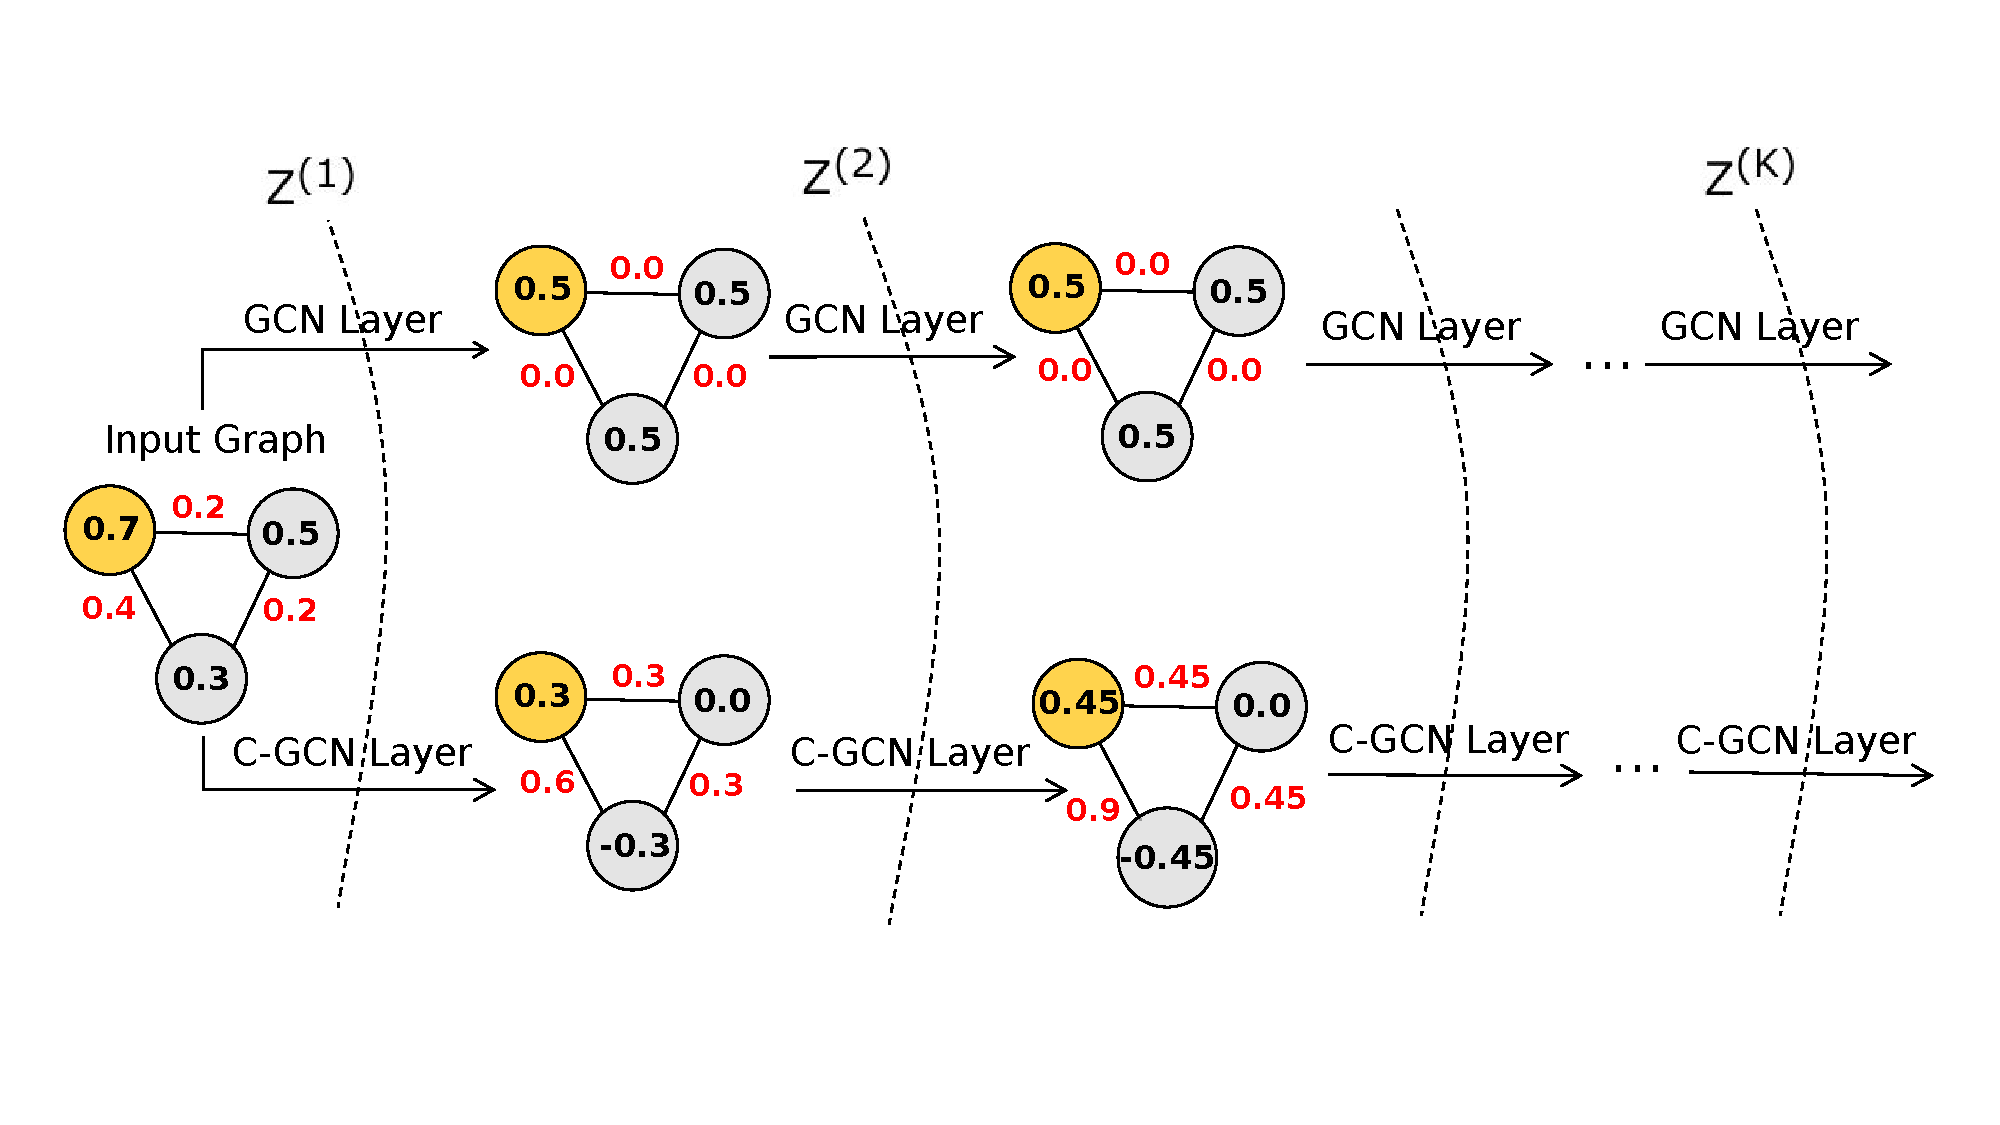
\includegraphics[scale=0.24]{figures/fig_contrast}
%   \caption{\small \label{fig:contrast}Stylized example showing the convolution results of GCN and proposed Contrastive GCN for a question with three answers. Edge labels denote the feature difference while node labels denote the resulting feature value. The feature difference between neighboring nodes increases with each convolution layer for Contrastive GCN while GCN averages the feature values among nodes. }
%     \vspace{-0.02mm}
% \end{figure}


% %For contrastive relation between, equation \ref{eq: GCN} will result in assigning feature of each answer $X_a, \forall a \in A(q)$ to question $q$, to the average of all other answers in the clique.
% %In the case of the contrastive relationship between answers, neighborhood averaging \emph{decreases} the difference between feature values of accepted and non-accepted answer and facilitates label sharing among all answers. Consider this stylized example, there are three answers $a_1$, $a_2$ and $a_3$ for question $q$ with $a_1$ being the accepted answer as shown in Figure \ref{fig:example}. Each answer has a single feature value $X$ with values being $X_{a,1} = 0.8, X_{a,2} = 0.1$ and $X_{a,3} = 0.3$. After single graph convolution operation with Identity weight matrix $W$, new feature values will be $\tilde{X}_{a,1} = \tilde{X}_{a,2} = \tilde{X}_{a,3}$ $= \sfrac{1}{3}[0.8 + 0.1 + 0.3]= 0.4$. As resulting average feature value is closer to the feature values of non-accepted class, each answer will be assigned non-accepted. This problem becomes more prominent with an increase in clique size or number of answers as neighborhood average will shift towards the non-accepted class. Note that as we are operating on a clique, subsequent graph convolutions do not change the result. Therefore, the original GCN framework is not able to identify the contrastive features of accepted answer against other non-accepted answers. This leads to misclassification of the accepted answer as the majority class of the clique, i.e., non-accepted.

% %\end{comment}

% %Most GCN based classification methods \cite{} employ a similar structure to that shown in Equation \ref{eq: GCN}, averaging of neighborhood features for each node in the graph. This approach does not work for contrastive relation setting where all neighbors need not share a class label. While there have been extensions of graph convolution to the inductive setting \cite{graphsage}, multi-relational setting \cite{relationalGCN}, and signed networks \cite{signedgcn}, none of these approaches are suitable for capturing data induced contrastive relation.

\subsection{Contrastive Graph Convolution}
\label{subsec:contrast}
% The contrastive relational view encodes contrast of each node to its neighborhood, a complementary hypothesis to the label sharing effect described in the previous section. We revisit a key simplifying assumption in \cite{gcn}, $\theta = \theta_{0} = -\theta_{1}$. This implictly encodes the similarity assumption in feature transformation.

Now, we show how to perform graph convolution to encode the mechanism of contrast, where label assignments for a tuple depend on the contrast with its neighborhood.

To establish contrast, we need to compute the \emph{difference} between the vertex's own features to its neighborhood in the clique. Thus we transform~\Cref{eq:restrictk} by setting $\theta = \theta_{0}$ = $\theta_{1}$, which essentially restricts the filters learned by the GCN. This transformation leads to the following convolution operation:
% $I_n$ and neighborhood averaged features $D^{-\frac{1}{2}}A_cD^{\frac{1}{2}}$ in the clique. We can encode this contrastive relationship by using same sign filter $\theta = \theta_{0}$ = $\theta_{1}$ which leads to this modified layer-wise convolution operation,
\begin{align}
%g_{\theta} * x &=  \theta_{0}x + \theta_{1}\left(L-I_{n} \right)x \\
g_{\theta} * x & =  \theta \left( I_N + L- I_{N} \right) x =  \theta \left( I_N - D^{-\sfrac{1}{2}} A D^{-\sfrac{1}{2}}\right) x \label{eq:contrastdetail}
% g_{\theta} * x \approx \theta\left(I_{n} - D^{-\sfrac{1}{2}}AD^{-\sfrac{1}{2}}\right)x,
\end{align}

Notice that~\Cref{eq:contrastdetail} says that for example, for any vertex $u$ with a scalar feature value $x_u$, for a given clique with $n \geq 2$ vertices, the convolution operation computes a new value $\hat{x}_u$ for vertex $u$ as follows:
\begin{equation}
  \hat{x}_u = \theta \left ( x_u - \frac{1}{n-1} \sum_{v \in \mathcal{N}_u} x_v \right ).
\end{equation}
where $\mathcal{N}_u$ is the neighborhood of vertex $u$. Notice that since our equivalence relations construct cliques, for all vertices $u$ that belong to a clique of size $n$, $|\mathcal{N}_u| = n-1$.

When we apply the convolution operation in~\Cref{eq:contrastdetail} at each layer of GCN, output for the $k$-th layer is:

% $\mathbf{Z}^{k-1}$ is the output of the previous $(k-1)^{th}$ layer, and $\mathbf{Z}^{0} = X$ with the input feature matrix $X$. $\mathbb{W}^{k}$ are filter $\theta$ paramters learnt by the network; $\sigma(.)$ denotes the activation function (e.g. ReLU, tanh).
% and the output of the $k^{th}$ convolutional layer is now given by,
\begin{equation}
  \label{eq:contrast}
  \mathbf{Z}_c^{k} = \sigma \left( \left (I_N - D^{-\sfrac{1}{2}}A_cD^{\sfrac{1}{2}} \right) \mathbf{Z}_c^{k-1} \mathbf{W}_c^{k}\right)
\end{equation}
with $A_c$ denoting the adjacency matrix in the contrastive view. $\mathbf{Z}_c^{k} \in \mathbb{R}^{N \times d}$ are the learned vertex representations for each $(q,a)$ tuple under the contrastive label assignment. $N$ is the total number of tuples and $d$ refers to the dimensionality of the embedding space. $\mathbf{Z}^{k-1}$ refers to the output of the previous $(k-1)$-{th} layer, and $\mathbf{Z}^{0} = X$ where $X$ is the input feature matrix. $\mathbf{W}_c^{k}$ are the filter $\theta$ parameters learnt by the GCN; $\sigma( \cdot)$ denotes the activation function (e.g. ReLU, $\tanh$).

% and $\mathbf{Z}_c^{k} \in \mathbb{R}^{\vert \mathcal{T} \vert \times d}$ are the learned node representations for each $(q,a)$ tuple under the contrastive strategy.

To understand the effect of~\Cref{eq:contrast} on a tuple, let us restrict our attention to a vertex $u$ in a clique of size $n$. We can do this since the convolution result in one clique is unaffected by other cliques. When we do this, we obtain:
\begin{equation}
  z_c^{k}(u) = \sigma \left(\left(z_c^{k-1}(u) - \frac{1}{n-1} \sum_{v \in \mathcal{N}_u} z_c^{k-1}(v) \right) \mathbf{W}_{c}^{k}\right). \label{eq:contrastrestrict}
  \end{equation}

% Note the effect of the change, each layer now computes the feature differences between each node and the local neighborhood, resulting in feature discrimination between contrasting nodes. Now we visit the term $(I_N - D^{-\sfrac{1}{2}}A_cD^{\sfrac{1}{2}}) \mathbf{Z}_c^{k-1}$. Under this formulation, the convolved feature value for node $i$, with neighborhood set $\mathcal{N}_i$ is given by,
% \begin{equation}
% z_c^{k}(i) = \sigma \left(\left(z_c^{k-1}(i) - \frac{1}{|\mathcal{N}_i|}\sum_{j \in \mathcal{N}_i}z_c^{k-1}(j)\right)\mathbf{W}_{c}^{k}\right)
% \end{equation}
Now consider a pair of contrasting vertices, $u$ and $v$ in the same clique of size $n$. Let us ignore the linear transform by setting $W_{c}^{k}=\mathbf{I}$ and set $\sigma(\cdot)$ to the identity function. Then we can easily verify that:

% immediate neighborhood of each other. Note that in our contrastive relational view, the nodes within each question have identical degree (say $d = |A_q|$).
\begin{equation}
z_c^{k}(u) - z_c^{k}(v) = \underbrace{
  \left (1 + \frac{1}{n-1} \right )
  }_{\text{magnification}}
  \times
  \underbrace{
    \left ( z_c^{k-1}(u) - z_c^{k-1}(v) \right )
    }_{\text{contrast in previous layer}}, \label{eq:disccontrastsimple}
\end{equation}
where, $z_c^{k}(u)$ denotes the output of the $k$-th convolution layer for the $u$-th vertex in the contrastive view. As a result, each convolutional layer magnifies the feature contrast between the vertices that belong to the same clique. Thus, the contrasting vertices move further apart. We term this as \emph{Discriminative Feature Magnification} and~\Cref{eq:disccontrastsimple} implies that we should see higher magnification effect for smaller cliques.
% An illustration is provided in the bottom part of the \cref{fig:contrast} with a uni-dimensional feature.

%Contrasting nodes are shifted further apart by \cref{eq:contrast} improving their separability in the learned manifold (further discussion in \cref{ref:analysis}).

% In our earlier example in Figure \ref{fig:example}, after applying proposed Contrastive GCN, new features values will be; $\tilde{X}_{a_1} = 0.8 - \frac{1}{2}[0.1 + 0.3] = 0.6$, $\tilde{X}_{a_2} = 0.1 - \frac{1}{2}[0.8 + 0.3] = -0.45$ and $\tilde{X}_{a_3} = 0.3 - \frac{1}{2}[0.8 + 0.1] = -0.15$.
%%For instance, in the answer selection problem, one or few of the set of answers to each question are accepted. Our objective is then to capture the contrast relation that exists between accepted answers and those that are not accepted.
%
%%\begin{comment}
%Each answer needs to \emph{contrast} between itself and rest of the answers. This can be achieved by computing the \emph{difference} instead of addition between node's own features $I_n$ and averaged features of the other nodes $D^{-\frac{1}{2}}A_cD^{\frac{1}{2}}$ in the clique. We can encode this contrastive relationship by using same sign filter $\theta = \theta_{0}$ = $\theta_{1}$ which leads to this modified layer wise convolution operation,
%\begin{equation}
%g_{\theta} * x \approx \theta\left(I_{n} - D^{-\frac{1}{2}}AD^{-\frac{1}{2}}\right)x,
%\end{equation}
%
%Thereby, output of the $k$-th hidden layer for Contrastive GCN network $Z_c^{(k)}$ is defined as:
%\begin{equation}
%  \label{eq:contrast}
%  Z_c^{(k)} = \sigma \left((I_n - D^{-\frac{1}{2}}A_cD^{\frac{1}{2}}) Z_c^{(k-1)}W_c^{(k)}\right)
%\end{equation}
%with $A_c$ as the Adjacency matrix with contrastive edges. In our earlier example in Figure \ref{fig:example}, after applying proposed Contrastive GCN, new features values will be; $\tilde{X}_{a_1} = 0.8 - \frac{1}{2}[0.1 + 0.3] = 0.6$, $\tilde{X}_{a_2} = 0.1 - \frac{1}{2}[0.8 + 0.3] = -0.45$ and $\tilde{X}_{a_3} = 0.3 - \frac{1}{2}[0.8 + 0.1] = -0.15$.
%
%\textbf{Disciminative Magnification} Note that this contrastive filter magnifies the difference between two classes, as difference between feature values, $X_{a,1}$ to $X_{a,2}$ and $X_{a,3}$ increased from $0.7$ and $0.5$ to $1.05$ and $0.75$. Stacking of this contrastive convolution layer with transformed features using $W$ weight matrix learns to magnifies the separation between features of accepted and non accepted class. This effect can be called as \emph{discriminative magnification} which improves the separation of nodes of different classes. This convolution still preserves the label sharing assumption between nodes of same class as their convolved features $\tilde{X}_{a_2} = -0.45$ and $\tilde{X}_{a_3} = -0.15$ are in similar range.

%Note that effectively the linear transformation averages the locality of a node and transforms the result linearly, layer to layer. This operation encodes an implicit notion of homophily in node classification. Nodes in similar localities or sharing neighbors are more likely to be assigned similar convolved feature representations. Alternative aggregation methods such as mean-pooling and max-pooling \cite{graphsage} achieve similar results.
%\end{comment}

 %While this does not necessarily improve the classification performance of conventional classifiers, the high VC dimension of neural networks can enable margin fitting to arbitrary regions in a high dimensional space.

%Alternately, we propose a much simpler solution to achieving node-feature contrast across convolutional layers.
%We analyze the implications of stacking the proposed convolutional contrast layers and analyze model performance in \cref{ref:analysis}.

%Also, signed edges are manually created. While graph attention networks with separate attention weight learned for each neighbor could learn negative attention weights for neighbors. However, it would be much more computationally expensive.

\subsection{Encoding Similarity Convolution}
\label{subsec:similar}
We next discuss how to encode the mechanism of sharing labels in a GCN. While label sharing applies to our similarity by contrast relation (two strategies: Arrival similarity; TrueSkill similarity, see~\Cref{sub:Induced Views}), it is also trivially applicable to the reflexive relation, where the label of the tuple only depends on itself. First, we discuss the case of similarity by contrast.

\subsubsection{Encoding Similarity by Contrast}
\label{sub:Encoding Similar Contrasts}

To encode label sharing for the two similarity by contrast cases, we transform~\Cref{eq:restrictk} with the assumption $\theta = \theta_0 = -\theta_1$. Thus

\begin{equation}
g_{\theta} * x = \theta\left(I_{N} + D^{-\sfrac{1}{2}}AD^{-\sfrac{1}{2}}\right) x, \label{eq:similargcn}
\end{equation}

%\Cref{eq:similargcn} says that for example, for any node $u$ with a scalar feature value $x_u$, for a given clique with $n\geq 2$ nodes,
Similar to the ~\Cref{eq:contrastdetail} analysis, convolution operation in \Cref{eq:similargcn} computes a new value $\hat{x}_u$ for vertex $u$ as follows:
\begin{align}
  \hat{x}_u &= \theta \left ( x_u + \frac{1}{n-1} \sum_{v \in \mathcal{N}_u} x_v \right ) = \theta \left ( \frac{n-2}{n-1} x_u + \frac{n}{n-1} \mu_x \right ).
\end{align}
That is, in the mechanism where we share labels in a clique, the convolution pushes the values of each vertex in the clique to the average feature value, $\mu_x = \frac{1}{n} \sum_{v \in \mathcal{N}_u \cup u} x_v$, in the clique.

When we apply the convolution operation in~\Cref{eq:similargcn} at each layer of GCN, output for the $k$-th layer:

% $\mathbf{Z}^{k-1}$ is the output of the previous $(k-1)^{th}$ layer, and $\mathbf{Z}^{0} = X$ with the input feature matrix $X$. $\mathbb{W}^{k}$ are filter $\theta$ paramters learnt by the network; $\sigma(.)$ denotes the activation function (e.g. ReLU, tanh).
% and the output of the $k^{th}$ convolutional layer is now given by,
\begin{equation}
  \label{eq:similar}
  \mathbf{Z}_s^{k} = \sigma \left( \left (I_N + D^{-\sfrac{1}{2}}A_sD^{\sfrac{1}{2}} \right) \mathbf{Z}_s^{k-1} \mathbf{W}_s^{k}\right)
\end{equation}
with $A_s$ denoting the adjacency matrix in the similar views.
%and $\mathbf{Z}_s^{k} \in \mathbb{R}^{N \times d}$ are the learned node representations for each $(q,a)$ tuple under the similar label assignment.
% $N$ is the total number of tuples,
% and where $d$ refers to the dimensionality of the embedding space. $\mathbf{Z}^{k-1}$ refers to the output of the previous $(k-1)$-{th} layer, and $\mathbf{Z}^{0} = X$ where $X$ is the input feature matrix. $\mathbf{W}^{k}$ are the filter $\theta$ parameters learnt by the GCN; $\sigma( \cdot)$ denotes the activation function (e.g. ReLU, $\tanh$).

We analyze the similarity GCN in a maner akin to~\Cref{eq:contrastrestrict} and
%consider a pair of similar nodes, $u$ and $v$ in the same clique of size $n$. Again, let us ignore the linear transform by setting $W_{c}^{k}=\mathbf{I}$ and set $\sigma(\cdot)$ to the identity function.Then
we can easily verify that:

% immediate neighborhood of each other. Note that in our contrastive relational view, the nodes within each question have identical degree (say $d = |A_q|$).
\begin{equation}
z_s^{k}(u) - z_s^{k}(v) = \underbrace{
  \left (1 - \frac{1}{n-1} \right )
  }_{\text{reduction}}
  \times
  \underbrace{
    \left ( z_s^{k-1}(u) - z_s^{k-1}(v) \right )
    }_{\text{contrast in previous layer}}, \label{eq:diffsimilar}
\end{equation}
where, $z_s^{k}(i)$ denotes the output of the $k$-th convolution layer for the $i$-th vertex in the similar view. As a result, each convolutional layer reduces the feature contrast between the vertices that belong to the same clique. Thus, the similar vertices move closer.

% As we observed in~\Cref{sub:Generalized Views}, three of our strategies---reflexive

% similarity relationships in the convolution framework. Recall from our discussion in ~\cref{sec:motivation}, a similarity edge connects two answers of a player if the contrast with the skill of other players answering the same question is identical. As similarity relation enforce smoothness or sharing of labels among nodes, we can directly apply the vanilla formulation (Equation \ref{eq:GCN}).
%Thus, the output of the $k$-th convolutional layer for the similarity view, $Z_s^{(k)}$ is defined as:
%\begin{equation}
%  \label{eq:similarity}
%  Z_s^{k} = \sigma \left((I_N + D^{-\frac{1}{2}}A_sD^{\frac{1}{2}}) Z_s^{(k-1)}W_s^{(k)}\right)
%\end{equation}
% However, for our experiments, we report better results without using renormalization trick.
%In this section, we showed how to encode the similarity mechanism where we share labels amongst vertices that belong to the same clique.

The proposed label sharing encoding applies to both similarity by contrast strategies (TrueSkill; Arrival). We refer to the corresponding vertex representations as $\mathbf{Z}_{ts}^{k}$ (TrueSkill), $\mathbf{Z}_{as}^{k}$ (Arrival).

%Recall from our discussed in Section \ref{sec:motivation}, a similarity edge connects two answers of a player if the contrast with the skill of other players answering the same question is identical. This follows from the principle that if there is a top ranked player, even if other players in the game have decent rankings, he would outplay all of them. In such scenarios, such contrastive answers from the top ranked player ought to share label and thus form a clique. Similar argument follows for the opposite case when you are outranked by all players in the game. We operationalize contrastive similarity using two data induced relationships.

%\textbf{True Skill Similarity} connects answers of the same answerer where difference in skill value of the answerer with other answerers for a question has a significant margin $\delta$. We estimate user's skill value using TrueSkill rating system \cite{TrueSkill06} computed on the basis of accepted label of user's all answers in the community.
%
%% developed by Microsoft Reasearch for ranking and matching similar skill game players for Xbox Live. In our settings, each question is a multi player game with all answerers as game players. The user who gives credible answer is the winner. True Skill rating then computes player's skill through bayesian inference on the basis of credibility label of his answered questions. The estimated ratings are a Gaussian distribution where $\mu$ denotes the average skill of the player. We use the mean value as skill value for our computations.
%
%Therefore, each user can have at most two cliques, one which connects all his answers where his true skill is significantly better than other answerers of the question; and second where his skill is vastly lower than all the other answerers. In the first case, he is highly likely to give accepted answers while in other, his answer would be classified as non-accepted. As CQA platforms encompass variety of topics, each user can be accepted in one topic while non accepted for other topics in the same community. \\MARGIN?
%Formally, output of the $k$-th hidden layer for True Skill Similarity GCN network $Z_{ts}^{(k)}$ is defined as:
%\begin{equation}
%  \label{eq:TSsimilarity}
%  Z_{ts}^{k} = \sigma\left((I_N + D^{-\frac{1}{2}}A_{ts}D^{\frac{1}{2}}) Z_{ts}^{(k-1)}W_s^{(k)} \right)
%\end{equation}
%with $A_{ts}$ being the adjacency matrix for true skill similarity relations.
%
%

%Thus, for each user, we construct a clique of all answers in which he answers significantly earlier than other answers, and another clique with all answers in which his answer is much later than all other answers for that question. Formally, output of the $k$-th hidden layer for Arrival Similarity GCN network $Z_{as}^{(k)}$ is defined as:
%\begin{equation}
%  \label{eq:ASsimilarity}
%   Z_{as}^{k} = \sigma \left((I_N + D^{-\frac{1}{2}}A_{as}D^{\frac{1}{2}}) Z_{as}^{(k-1)}W_s^{(k)} \right)
%\end{equation}
%with $A_{as}$ being the adjacency matrix for arrival similarity relationship.

\subsubsection{Reflexive Convolution}
\label{subsubsec:reflex}
We encode the reflexive relation with self-loops in the graph resulting in an identity adjacency matrix. This relation is the trivial label sharing case, with an independent assignment of vertex labels. Thus, the output of the $k$-th convolutional layer for the reflexive view, $\mathbf{Z}_r^{k}$ reduces to:
\begin{equation}
  \label{eq:reflexive}
  \mathbf{Z}_r^{k} = \sigma \left( I_N \mathbf{Z}_r^{k-1} \mathbf{W}_r^{k} \right)
\end{equation}
Hence, the reflexive convolution operation is equivalent to a feedforward neural network with multiple layers and activation $\sigma( \cdot )$.

\vspace{0.1in}
\noindent
%Each strategy $i \in \mathbf{S}$ produces a view $G_i = (V, E_i)$ with identical vertex set $V$.
Each strategy $S_i \in \mathbf{S}$ belongs to one of the three relation types---reflexive, contrastive and similarity, where $\mathbf{R}$ denotes the set of strategies of that relation type. $\mathcal{R} = \bigcup \mathbf{R}$ denotes the set of all relation types.
%We apply all strategies on each vertex $v \in V$ corresponding to tuple $(q,a)$.
%We combine the results of the embeddings from the each of the four strategies as follows. Let $v \in V$ correspond to the tuple $(q,a)$.
$\mathbf{Z}_i^K \in \mathbb{R}^{N X d}$ represents the $d$ dimensional vertex embeddings for strategy $S_i$ at the $K$-th layer. For each strategy $S_i$, we obtain a scalar score by multiplying $\mathbf{Z}_i^K$ with transform parameters $\widetilde{W}_i \in \mathbb{R}^{d \times 1}$.
%Each strategy $\mathbf{S}_k$ produces a view $G_i = (V, E_i)$ with identical vertex set $V$. We apply each of the $i=4$ strategies $\mathbf{S}_k \in \mathcal{S}$ on each vertex $v \in V$ corresponding to tuple $(q,a)$. We combine the results of the embeddings from the each of the four strategies as follows. Let $v \in V$ correspond to the tuple $(q,a)$. Let $\mathbf{Z}_i^K(v)$ be the the $d$ dimensional embedding for node $v$, strategy $i$ at the $K$-th layer. For each strategy $i$, we project $\mathbf{Z}_i^K(v)$ to a scalar using transform parameters $\widetilde{W}_i \in \mathbb{R}^{d \times 1}$.
%Thus, for each relation type $\mathbf{R} \in \mathcal{R}$, and their corresponding views $i \in \mathbf{R}$, their convolution generates node representations $\mathbf{Z}_{i}^{K} \in \mathbb{R}^{N \times d}$ for each node $v \in V$. Each $Z_{i}^{K}$ is projected to generate a single score or prediction outcome for that view using transform parameters $\widetilde{W}_i \in \mathbb{R}^{d \times 1}$.
The sum of these scores gives the combined prediction score, $\mathbf{H}_{\mathbf{R}} \in \mathbb{R}^{N X 1}$, for that relation type.
%of all strategies, $S_i \in \mathbf{R}$.
%relation type $\mathbf{R}$ for each node over the graph convolutions with the different views $G_i , \forall i \in \mathbf{R}$ of that relation type,
\begin{equation}
    \label{eq:score}
        \mathbf{H}_{\mathbf{R}} = \sum_{S_i \in \mathbf{R}} \mathbf{Z}_i^K \widetilde{W}_i^T
\end{equation}

%The induced views under \emph{Similarity by contrast} strategy semantically differ from the view under \emph{Contrastive} strategy in two ways. First, they enable feature sharing between the connected nodes. In the \emph{Contrastive} strategy, the objective is feature discrimination; a node that contrasts with its neighbors is likely to have a different label. These semantics are captured in the convolutional architecture we apply to those views (\cref{subsec:contrast}, \cref{subsec:similar}). Second, since there are multiple ways to construct \emph{Similarity by contrast} views, they depend on the similarity measure (TrueSkill and Arrival Similarity are two relevant metrics in CQA). Views within a strategy are likely to be correlated. Our architecture combines cross-strategy and intra-strategy views appropriately to encode this difference (\cref{sec:aggregation}).

In this section, we proposed Graph Convolutional architectures to compute vertex representations of each $(q,a)$ tuple under the four strategies. %Each strategy induces cliques and used one of three relationship types---\textit{contrastive}, \textit{similar contrast} and \textit{reflexive}.
%Each strategy induces cliques, and within a clique
In particular, we showed how to encode two different label assignment mechanisms---label sharing and determine label based on contrast---within a clique. The architecture that encodes label assignment based on contrast is a novel contribution, distinct from the formulations presented by Kipf et al.~\cite{gcn} and its extensions~\cite{signedgcn,relationalGCN}. Prior convolutional architectures implicitly encode the label sharing mechanism (~\cref{eq:similargcn}); however, label sharing is unsuitable for contrastive relationships across vertices. Hence our architecture fills this gap in prior work.

%Now, we proceed to develop and compare aggregation approaches to combine the predictions of the different strategies.
%\clearpage

\section{Aggregating Induced Views}
\label{sec:aggregation}
In the previous sections, we introduced four strategies to identify the accepted answer to a question. Each strategy induces a graph or relational view between $(q,a)$ tuples.
%three relation types to connect $(q,a)$ tuples --- Contrastive, Similar Contrast and Reflexive. Each relation type has one or more induced views capturing relationships between $(q,a)$ tuples under a strategy. %We distinguish the relational class and a specific view such as TrueSkill, which is an instance of the Similarity class.
Each relational view is expected to capture semantically diverse neighborhoods of vertices. The convolution operator aggregates the neighborhood information under each view. The key question that follows is, \emph{how do we combine these diverse views in a unified learning framework?} Past work has considered multiple solutions:
\begin{itemize}
  \label{item:aggregator}
\item \textbf{Neighborhood Aggregation}: In this approach, we represent vertices by aggregating feature representations of it's neighbors across all views \cite{graphsage,relationalGCN}.
\item \textbf{Stacking}: Multiple convolution layers stacked end-to-end (each potentially handling a different view) \cite{Stacking}.
\item \textbf{Fusion}: Follows a multi-modal fusion approach~\cite{Fusion18}, where views are considered distinct data modalities.
\item \textbf{Shared Latent Structure}: Attempts to transfer knowledge across relational views (modalities) with constraints on the representations (e.g. \cite{DualGCN} aligns embeddings across views).
\end{itemize}

Ensemble methods introduced in \cite{relationalGCN} work on multi-relational edges in knowledge graphs. None of these approaches are directly suitable for our induced relationships. Our relational views utilize different label assignment semantics (label sharing within a clique vs. determine label based on contrast within a clique). In our label contrast semantics, we must achieve feature discrimination and label inversion between contrasting vertices, as opposed to label homogeneity and feature sharing in the label sharing case. Thus, aggregating relationships by pooling, concatenation, or addition of vertex representations fail to capture semantic heterogeneity of the induced views.
Further, data induced relations are uncurated and inherently noisy. Directly aggregating the learned representations via Stacking or Fusion can lead to noise propagation. We also expect views of the same relation type to be correlated.

%In our Contrastive strategy, we must achieve feature discrimination and label inversion between contrasting nodes, as opposed to label homogeneity and feature sharing in the Relative Similarity strategy. Gradient boosting techniques are known to improve performance when individual classifiers, including neural networks \cite{ncboost}, are diverse yet accurate. A natural solution then is to apply boosting to the set of IR-GCNs and bridge the weaknesses of each learner. However, a direct application across all views is sub-optimal as it does not exploit the commonalities within a strategy (e.g., The TrueSkill and Arrival Similarity views within Relative Similarity).

%\begin{itemize}
%\item \textbf{Consistency Viewpoint:} In this view, each relation GCN is though to produce precisely the same result in the ideal case, i.e., where they are all trained exhaustively on the chosen set of relations. Thus, the reduced performance is though to indicate incompleteness rather than inability. Namely, aligning the relation GCNs in a co-operative manner is thought to produce the best results. Recent work \cite{www2018} used local and global neighborhoods of nodes (by random-walk similarity) to construct a pair of aligned GCNs. They further introduced a regularization or result-alignment term in the loss function to improve their performance by leveraging each other's predictions.
%
%\item \textbf{Diversity Viewpoint:} Conversely, in this view, each relation GCN is though to fit to a different subset of the data points. For instance Contrast relation is likely to perform well in the presence of a single quality answer while True Skill similarity identifies the relative position of users in comparison to their peers. Unlike the pretvious case, the ideal outcome in the Diversity viewpoint is to learn completely disjoint relation GCNs, each of which perform well on some subset of the data or the input feature space. It is easy to bserve that the best strategy in this case is not to try and align the GCNs. Rather, we must effectively exploit their dissimilarities to obtain the best combined performance.
%\end{itemize}

\begin{figure}
    \centering
        %\includegraphics[width=\columnwidth,height=3cm]{figures/model.pdf}
    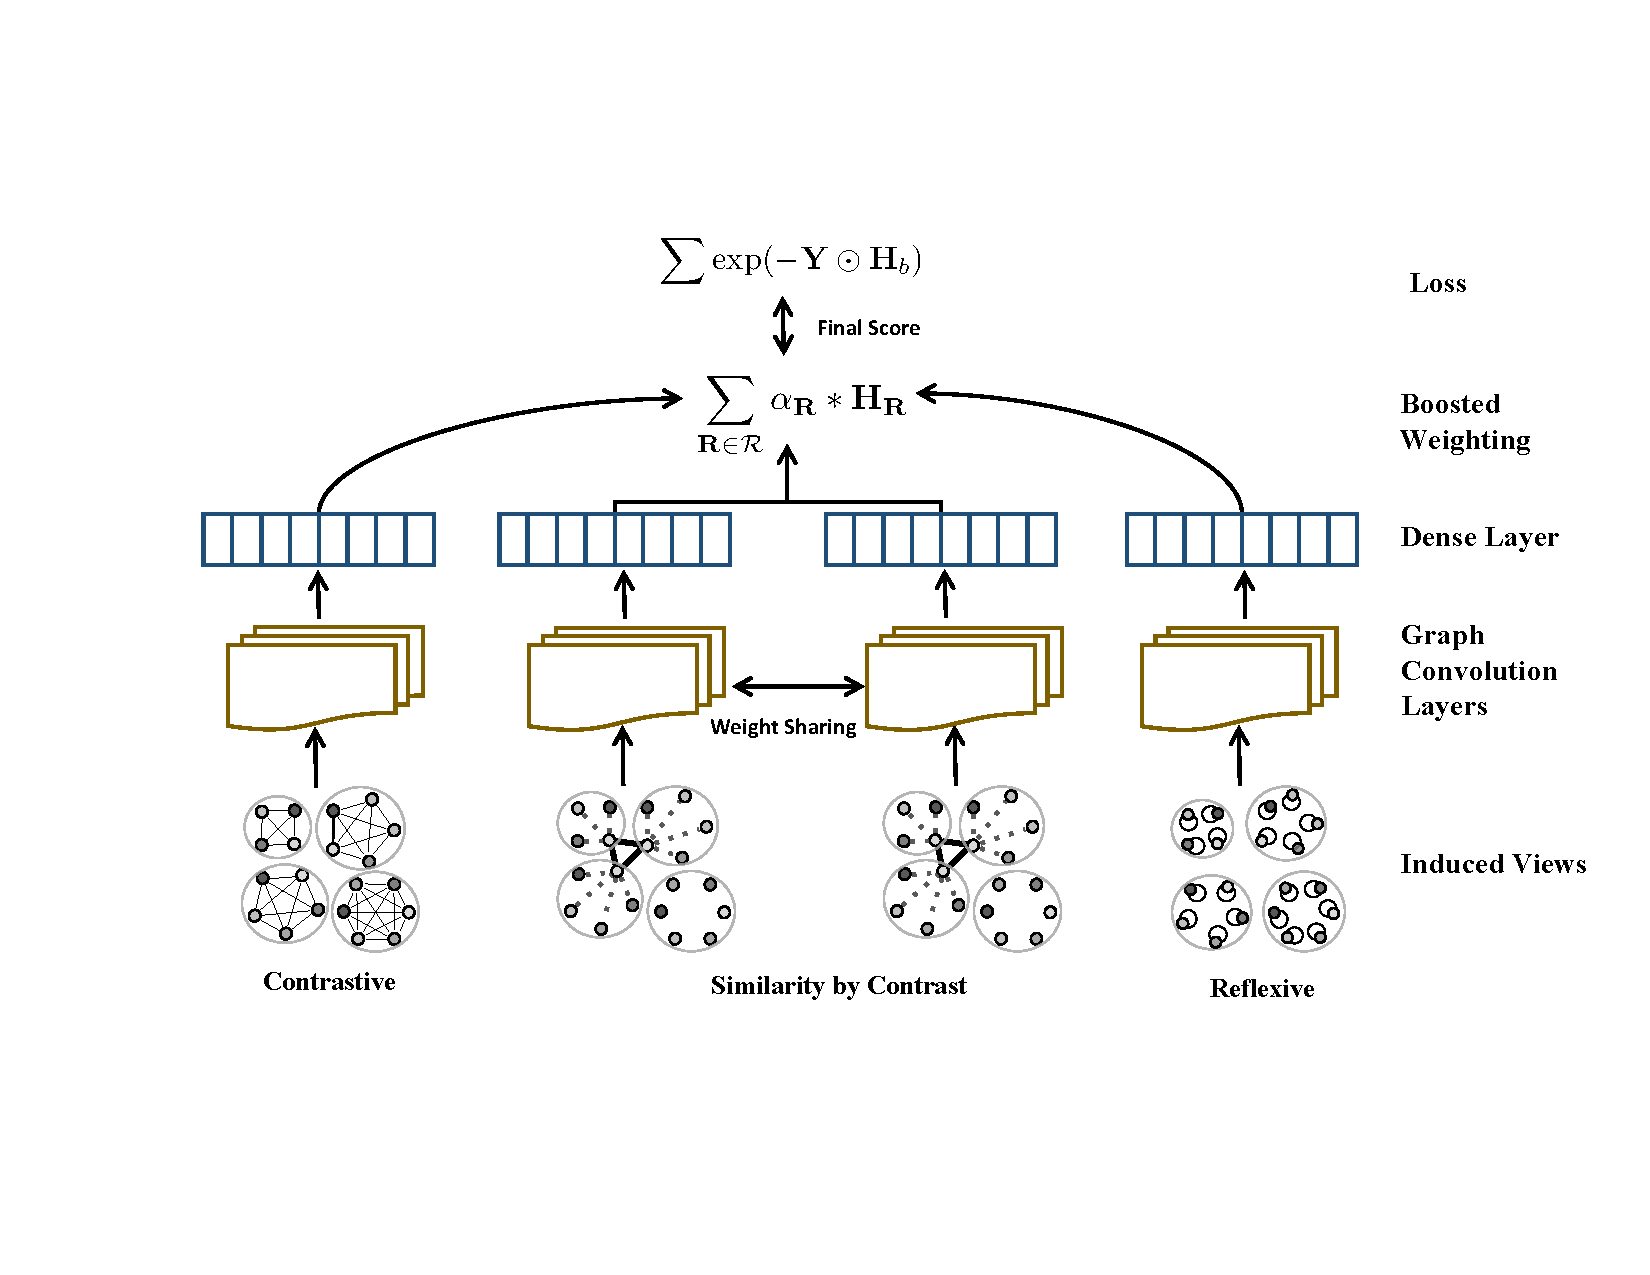
\includegraphics[scale=0.48]{figures/Architecture_new.pdf}
    %\includegraphics[scale=0.33]{figures/Architecture_dark.pdf}
    \caption{\small \label{fig:adaboost} Schematic diagram of our proposed IR-GCN model.} %The model is generic and can be extended to relational classes and multiple relational views within each class.}
    \vspace{-0.1in}
\end{figure}

%Consider the most general ontology of the chosen relations, namely a set of strategies (such as Contrastive and Similarity), each with multiple views (e.g. True Skill, Arrival).

We thus propose the following approach to aggregate information across relation types and between views of a relation type.

\noindent
\textbf{Cross-relation Aggregation}: We expect distinct relation types to perform well on different subsets of the set of $(q,a)$ tuples. We empirically verify this with the Jaccard overlap between the set of misclassified vertices under each relational view of a relation type on our dataset. Given $\mathbf{M}_A$ and $\mathbf{M}_B$, the sets of $(q,a)$ tuples misclassified by GCNs $A$ and $B$ respectively, the jaccard overlap is,
\begin{equation*}
 \mathcal{J}_{A,B} = \frac{\mathbf{M}_A \cap \mathbf{M}_B}{\mathbf{M}_A \cup \mathbf{M}_B}
\end{equation*}
The $\mathcal{J}_{A,B}$ values are as follows for the relational pairings: (Contrastive, TrueSkill Similarity) = 0.42, (Contrastive, Reflexive) = 0.44 and (Reflexive, TrueSkill Similarity) = 0.48. Relatively low values of the overlap metric indicate uncorrelated errors across the relations.

Gradient boosting techniques are known to improve performance when individual classifiers, including neural networks \cite{ncboost}, are diverse yet accurate. A natural solution then is to apply boosting to the set of relation types and bridge the weaknesses of each learner. We employ Adaboost \cite{adaboost} to combine relation level scores, $\mathbf{H}_{\mathbf{R}}$ (~\cref{eq:score}) in a weighted manner to compute the final boosted score, $\mathbf{H}_b \in \mathbb{R}^{N \times 1}$ representing all relation types (Line 12, ~\cref{alg:inference}). $\mathbf{Y} \in \mathbb{R}^{N X 1}$ denotes the acceptance label of all tuples. Note that an entry in $(\mathbf{Y} \odot \mathbf{H_{\mathbf{R}}}) > 0 $ when the accepted label of the corresponding $(q,a)$ tuple and sign of the prediction score, $sign(\mathbf{H_{\mathbf{R}}})$, of relation type $\mathbf{R}$ match and $< 0$ otherwise. Thus, the weights $\alpha_\mathbf{R}$ adapt to the fraction of correctly classified tuples to the misclassified tuples by the relation $\mathbf{R}$ (Line 9, ~\cref{alg:inference}).
%weight of each subsequent strategy's score is determined by the misclassification error, ($\mathbf{e}_\mathbf{S}$), of $(q, a)$ tuples by the current set of strategies.
The precise score computation is described in ~\cref{alg:inference}. We use the polarity of each entry in the boosted score, $sign(\mathbf{H}_b) \in \{-1,1 \}$, to predict the class label of the corresponding $(q,a)$ tuple. The final score is also used to create a ranked list among all the candidate answers, $a \in \mathcal{A}(q)$ for each question, $q \in \mathcal{Q}$. $L_{(q,a)}$ represents the position of candidate answer $a$ in the ranked list for question $q$.

%These class level outputs are then scaled and combined by the respective gradient boosting methods (we employed Adaboost \cite{adaboost} in our experiments)
\begin{algorithm}
\caption{IR-GCN Boosted Score Computation}\label{alg:inference}
\begin{algorithmic}[1]
%\Require{Nodes $x_1 \ldots x_n$, Class labels $y_1 \ldots y_n$, $y_i \in \{-1,1\}$, Adjacency matrix of each induced GCN $A_c, A_{ts}, A_{as}, A_r$}
%\Ensure{boosted score $h_b(x_i) \forall i \in [1, n]$}
\Function{Forward}{$\mathbf{X}, \mathbf{Y}, \{A_i\}_{S_i \in \mathbf{S}}$}
  \State $\mathbf{H}_{b} \gets \mathbf{0} $
    \For{$\mathbf{R} \in \mathcal{R}$}
    \State $\{ \mathbf{Z}_i^K \}_{S_i \in \mathbf{R}} \gets Conv(\mathbf{X}, \{ A_i \}_{S_i \in \mathbf{R}})$
    \State \Comment{Equation  \ref{eq:contrast}, \ref{eq:similar}, \ref{eq:reflexive}}
    \State $\mathbf{H}_\mathbf{R} =\sum_{{S_i} \in \mathbf{R}} \mathbf{Z}_i^{K} \times \widetilde{\mathbf{W}}_i$ \Comment{Equation \ref{eq:score}}
    %\State $h_s = merge(h_{as}, h_{ts})$ \Comment{Equation \ref{eq:merge}}
    \State $ \mathbf{e}_{\mathbf{R}} \gets \exp({-\mathbf{Y} \odot \mathbf{H}_{b}})$
    \State \Comment{ $\odot \rightarrow \textit{Hadamard Product}$}
  \State $\alpha_\mathbf{R} \gets \dfrac{1}{2} \ln{\dfrac{\sum \mathbf{e}_{\mathbf{R}} \odot \mathbbm{1}\left((\mathbf{Y} \odot \mathbf{H}_{\mathbf{R}}\right) > 0)}{\sum \mathbf{e}_{\mathbf{R}} \odot \mathbbm{1}\left((\mathbf{Y} \odot \mathbf{H}_{\mathbf{R}}) < 0 \right) }}$
    \State \Comment{$\sum \rightarrow \textit{reduce-sum}$}
      \State \Comment{$\mathbbm{1}(.) \rightarrow \textit{element-wise Indicator function}$}
  \State    $\mathbf{H}_{b} \gets \mathbf{H}_{b} + \alpha_\mathbf{R} * \mathbf{H}_{\mathbf{R}}$ \Comment{Update boosted GCN}
%    \State $ w_{i,r} \gets \exp^{-y_i * h_{cs}(x_i)}$
%  \State    $\alpha_r \gets \dfrac{1}{2} \lnb{\dfrac{\sum\limits_{y_i = h_s(x_i)} w^{i,c}}{\sum\limits_{y_i \neq h_s(x_i)} w_{i,c} }}$
%    \State $h_{b}(x_i) \gets h_{cs}(x_i) + \alpha_r * h_{cs}(x_i)$\Comment{Final Boosted GCN}
    \EndFor
    \State \Return $\mathbf{H}_{b}$, $ \{ \mathbf{H}_{R} \}_{\mathbf{R} \in \mathcal{R}}$, $\{ \mathbf{Z}_{i}^{K} \}_{S_i \in \mathbf{S}}$
    \State \Comment{Boosted scores, Relation level scores,}
    \State \Comment{Each GCN vertex representations}
\EndFunction
\end{algorithmic}
\end{algorithm}

%Now we describe the boosted weights for the outputs of each relational view for each tuple $t_{i}$, namely $h_{\mathcal{C}}(t_{i})$. The weights $w_{\mathcal{C}}(t_i)$ of the $t_i^{th}$ tuple for the $\mathcal{C}^{th}$ relational view are given by $w_{\mathcal{C}}(t_i) = e^{-y_{i}\times h_{(1 \ldots \mathcal{C}-1)}(t_i)}$, where $h_{(1 \ldots \mathcal{C}-1)}$ denotes the prediction output of the boosted classifier combining all relational views before view $\mathcal{C}$. In our answer selection problem, the contrastive relational view performs the best, and is hence added first to the ensemble, followed by relative similarity and reflexive views, i.e. $\{c,s,r\}$. The above description is formalized in \cref{alg:inference}.

\noindent
\textbf{Intra-relation Aggregation}: Gradient boosting methods can effectively aggregate relation level representations, but are not optimal within a relationship type (since it cannot capture shared commonalities between different views of a relation type). For instance, we should facilitate information sharing between the TrueSkill similarity and Arrival similarity views. Thus, if an answer is authored by a user with a higher skill rating and answered significantly earlier than other answers, its probability to be accepted should be mutually enhanced by both signals. Empirically, we also found True Skill and Arrival Similarity GCNs to commit similar mistakes ($\mathcal{J}_{TS,AS}$ = 0.66). Thus, intra-relation learning (within a single relation type like Similarity by Contrast) can benefit from sharing the structure of their latent spaces, i.e., weight parameters of GCN.

%We also share the weight matrices $W_{v}^{k} \forall k \in [1,\ldots,K]$ to enable analogous data transformations between TrueSkill and Arrival Similarity.



%Motivated by the regularization term in \cite{DualGCN}, we follow a similar strategy to combine our similiarity view IR-GCNs. Now consider a relational view $\mathcal{C}$ with instances $v \in \mathcal{C}$ (e.g. TrueSkill, Arrival in the Similarity view). To share the latent structure of their representations, the following regularizer is introduced ($t_i$ denotes a single $(q,a)$ tuple),
%\begin{equation}
%\sum_{i}\sum_{(v, v') \in \mathcal{C}} || Z_v^{K}(t_i) - Z_{v'}^{K}(t_i) ||
%\end{equation}
%The embedding representations are constrained to be similar at the last layer (k=K) for all pairs of instances in a view.


%We provide the details of our training algorithms in \cref{sec:aggregation}.

%In the previous sections we described three relational views, Contrastive (c), Similarity (s) and Reflexive (r). For each view $\mathcal{C} \in \{c,s,r\}$, we have a set of instances $v \in \mathcal{C}$ and each IR-GCN$_{v}$ generates embedding representation $Z_{v}^{K}(t_i)$.
%These class level outputs are then scaled and combined by the respective gradient boosting methods (we employed Adaboost \cite{adaboost} in our experiments). Figure \ref{fig:adaboost} exhibits the overall architecture of our Boosted IR-GCN model. The above description is formalized in \cref{alg:inference}.
\noindent
\emph{Weight Sharing:} For multiple views representing a relation type (e.g., TrueSkill and Arrival Similarity), we train a separate GCN for each view but share the layer-wise linear-transforms $\mathbf{W}_i^{k}$ to capture similarities in the learned latent spaces.
Weight sharing is motivated by a similar idea explored to capture local and global views in \cite{DualGCN}. Although sharing the same weight parameters, each GCN can still learn distinct vertex representations as each view convolves over a different neighborhood and employ random dropout during training.
%Thus, in practice, each view can potentially predict opposite class labels.
We thus propose to use an alignment loss term to minimize prediction difference between views of a single relation type\cite{reg}. The loss attempts to align the learned vertex representations at the \emph{last layer} $K$ (the loss term aligns pairs of final vertex representations, $\lvert\lvert \mathbf{Z}_i^{K} - \mathbf{Z}_{i'}^{K} \lvert\lvert \texttt{  }\forall\texttt{ } S_i, S_i' \in \mathbf{R}$). In principle, multiple GCNs augment performance of the relation type by sharing prior knowledge through multiple Adjacency matrices ($\mathbf{A}_i \texttt{  }\forall\texttt{ } S_i \in \mathbf{R}$).
%weight sharing and alignment loss.


\begin{algorithm}[tbh]
\caption{IR-GCN Training}\label{alg:training}
\begin{algorithmic}[1]
\Require{Input Feature Matrix $X$, Acceptance labels for each tuple, $\mathbf{Y}$, Adjacency matrix of each view $\{A_i\}_{S_i \in \mathbf{S}}$ }
\Ensure{Trained Model i.e. Weight parameters $W_{i}^{1} \ldots W_{i}^{k}, S_i \in \mathbf{S}, \forall k \in [1, K]$ and transform parameters $\widetilde{W}_i$, $S_i \in \mathbf{S}$ }
%\Ensure{Trained Model i.e. Weight parameters $W_{\mathbf{S}}^{1} \ldots W_{\mathbf{S}}^{k}, \mathbf{S} \in %\mathbb{S} $ and transform parameters $\widetilde{W}_v$, $v \in \mathbf{V}$ }
%\While{ $not$ $converged$}
%\For{$t\gets0 to \textit{num_epochs}$ }
\For{$t \gets 1$ to $\textit{num-epochs}$}
    \State $\mathbf{H}_b, \{ \mathbf{H}_{R} \}_{\mathbf{R} \in \mathcal{R}}, \{ \mathbf{Z}^{K}_{i} \}_{S_i \in \mathbf{S}}$$\gets \textsc{Forward}(X, Y, \{ A_i \}_{S_i \in \mathbf{S}})$
    \State \Comment{\Cref{alg:inference}}
    \For{ $\mathbf{R} \in \mathcal{R}$}

        \State $\mathcal L_b \gets \sum \exp({-\mathbf{Y} \odot \mathbf{H}_b}) + \gamma_1 \mathcal L_1(.) + \gamma_2 \mathcal L_2(.)$
    \State \Comment{$\sum \rightarrow \textit{reduce-sum}$}
  \State \Comment{$\odot \rightarrow \textit{Hadamard Product}$}
        \State $\mathcal L_{\mathbf{R}} \gets 0$
        \For{ $S_i \in \mathbf{R}$}
        \State $\mathcal L_{i} \gets \sum \exp({-\mathbf{Y} \odot \mathbf{H}_\mathbf{R}})$
                    %\State \Comment{$\sum \rightarrow \textit{reduce-sum}$}
    \State $\mathcal L_{\mathbf{R}} \gets \mathcal L_{\mathbf{R}} + \mathcal L_{i} + \frac{1}{2}\sum_{S_i' \neq S_i}\lvert\lvert \mathbf{Z}_{i}^K - \mathbf{Z}_{i'}^K \lvert\lvert $
    \EndFor
    \State $\mathcal L_b \gets \mathcal L_b + \lambda(t) \mathcal L_{\mathbf{R}}$
    \State    $W_i^{k} \gets  W_i^{k} + \eta_{\textsc{adam}} \frac{\partial \mathcal L_b}{\partial W_i^{k}} $ \Comment{$\forall k \in [1, K], \forall S_i \in \mathbf{R}$}
     \State    $\widetilde{W}_i \gets  \widetilde{W}_i +  \eta_{\textsc{adam}} \frac{\partial \mathcal L_b}{\partial \widetilde{W}_i}$ \Comment{$\forall S_i \in \mathbf{S}$}
    \EndFor
\EndFor
\end{algorithmic}
\end{algorithm}

%\subsection{Training algorithm}
\noindent
\textbf{Training Algorithm}: Algorithm \ref{alg:training} describes the training algorithm for our IR-GCN model. For each epoch, we first compute the aggregated prediction score $\mathbf{H}_{b}$ of our boosted model, as described in \cref{alg:inference}. We use a supervised exponential loss $\mathcal{L}_b$ for training with elastic-net regularization (L1 loss - $\mathcal L_1(.)$ and L2 loss - $\mathcal L_2(.) $) on the graph convolutional weight matrices $\mathbf{W}_{\mathbf{i}}^{k} \texttt{  }\forall\texttt{ } S_i \in \mathbf{S}$ for each view. Note that we employ weight sharing between all views of the same relation type so that only one set of weight matrices is learned per relation. %The views in our training are Contrast (c), TrueSkill (ts), Arrival Similarity (as), and Reflexive view (r).
The exponential loss, $\mathcal{L}_{\mathbf{R}}$, for each relation type is added alternatingly to the boosted loss.
We apply an \emph{exponential annealing schedule}, $\lambda(t)$, i.e. a function of the training epochs ($t$), to the loss function of each relation. As training progress and the boosted model learns to distribute vertices among the relations optimally, an increase in $\lambda(t)$ ensures more emphasis is provided to the individual convolutional networks of each relation. Figure \ref{fig:adaboost} illustrates the overall architecture of our IR-GCN model.

%\textbf{IR-GCN Annealing}:
%Note that the regularizer $\lvert\lvert Z_{as} - Z_{ts} \lvert\lvert$ ensures close coupling between the embeddings learned between views of the same strategy. F %The final output score of similarity relation is then computed by aggregating information from both relations as in Equation \ref{eq:merge}.




%We now consider Intra-class aggregation.

% Now we describe the boosted weights for the outputs of each relational view for each tuple $t_{i}$, namely $h_{\mathcal{C}}(t_{i})$. The weights $w_{\mathcal{C}}(t_i)$ of the $t_i^{th}$ tuple for the $\mathcal{C}^{th}$ relational view are given by $w_{\mathcal{C}}(t_i) = e^{-y_{i}\times h_{(1 \ldots \mathcal{C}-1)}(t_i)}$, where $h_{(1 \ldots \mathcal{C}-1)}$ denotes the prediction output of the boosted classifier combining all relational views before view $\mathcal{C}$. In our answer selection problem, the contrastive relational view performs the best, and is hence added first to the ensemble, followed by relative similarity and reflexive views, i.e. $\{c,s,r\}$. The above description is formalized in \cref{alg:inference}.


%Gradient boosting techniques are known to improve performance when individual classifiers, including neural networks \cite{ncboost}, are diverse yet accurate. This precisely fits our inter-class aggregation problem. The aggregate of the strongest relational class is added first to the ensemble, and adaptive weights are applied for each subsequent relational class to leverage the misclassified nodes of the current boosted classifier, hence satisfying the diversity viewpoint.



% Each $v^{th}$ IR-GCN produces an output score $h_v(t_i) \in [ -1, 1 ]$ for each tuple $t_i$. We obtain this score by projecting learned node embeddings $Z_m(x_i)$ for each IRGCN to a single value.
%\begin{equation}
%    \label{eq:score}
%        h_m(x_i) = Z_m(x_i) * \tilde{W}_m; \forall m \in \{ c, ts, as, r\}
%\end{equation}
%with $\tilde{W}_m \in \mathbb{R}^{K X 1}$ and output embedding size $K$. If there are multiple induced relations for a relationship type, final score is computed by concatenating scores of each induced-relation GCN model. For instance, for similarity relation, final score $h_s(x_i)$ is computed as,
%\begin{equation}
%    \label{eq:merge}
%    h_s(x_i) = [h_{ts}(x_i), h_{as}(x_i)]* \tilde{W}_{concat}
%\end{equation}
%where $h_{ts}$ is true skill similarity GCN score, $h_{as}$ is arrival similarity GCN score with $\tilde{W}_{concat} \in \mathbb{R}^{2 X 1}$.


%\vspace{-0.2in}
%We then combine these individual $h_m$ scores to compute final score of our boosted Induced-Relation GCN model as defined in Algorithm \ref{alg:inference}. We define weight $w_m^{(i)}$ of $m$th weak learner for node $x_i$ as the exponential loss over $m-1$th weak learner's score:
%\begin{equation}
%    \label{eq:weight}
%        w^{(i)}_m = \exp^{-y_i * h_{m-1} (x_i)}
%    \end{equation}
%For our answer selction problem, contrastive GCN is the strongest individual learner followed by similarity and reflexive GCN. We then compute weight for second weak learner, similarity GCN $w_s^{(i)}$ using line 7 in Algorithm \ref{alg:inference}. The weight of node $x_i$ for similarity GCN increases as the score of contrastive GCN $h_c$ is further away from the true label $y_i$. Final combined weight for similarity GCN learner $\alpha_s$ is proportional to the ratio of sum of weights $w_{i,s}$ for nodes $x_i$ correctly classified by similarity GCN with the sum of weights of misclassified nodes. This combined weight, hence, ensures that similarity GCN trains better for nodes misclassified by the contrastive GCN. The intermediate boosted score $h_{cs}$ is then defined as a weighted sum of Contrastive GCN score $h_c$ and Similarity GCN score $h_s$ in Line 9. The same process is repeated for reflexive learner where weight is determined using misclassification errors of the intermediate boosted learner. Line 12 specifies the final score for boosted induced-relation GCN $h_b$.

%
% \begin{algorithm}[H]
% \caption{Sum of Array Elements}
% \label{alg:loop}
% \begin{algorithmic}[1]
% \Require{Nodes $x_1 \ldots x_n$, Class labels $c_1 \ldots c_n$ ,$c_i \in \{-1,1\}$, Output of each induced GCN $h_c, h_s, h_r$ $\forall h: x \rightarrow \{ -1, 1 \}$}
% \Ensure{$h_G$ (Final label for each node)}
% \Statex
% \Function{Loop}{$A[\;]$}
%   \State {$Sum$ $\gets$ {$0$}}
%     \State {$N$ $\gets$ {$length(A)$}}
%     \For{$k \gets 1$ to $N$}
%         \State {$Sum$ $\gets$ {$Sum + A_{k}$}}
%     \EndFor
%     \State \Return {$Sum$}
% \EndFunction
% \end{algorithmic}
% \end{algorithm}
%\setlength{\textfloatsep}{1pt}
%The contrastive, similarity and reflexive relations capture different facets of question-answer pairs as a function of their competitors, similar tournaments and self-features. Each induced relationship captures a different data characteristic and the convolution operation aggregates neighborhood information from each of these relationships. The key question that follows is, how do we combine these diverse sources of relationship information in a unified learning framework? We first analyze the relative strengths of each learner by comparing the set of nodes they can correctly classify when applied in isolation.
% A combined classification model could thus outperform individual learners by a wide margin.
%
%%Thus, it is important to combine these different information to build an effective classification model.
%%To verify correlation between these relationships, we compute Jaccard Coefficient between the misclassified nodes of Contrastive, True Skill Similarity and Reflexive GCN model.
%Total loss of our proposed model is then defined as weighted sum of boosted model loss $\mathcal L_b$ with loss for similarity relation GCN. The weight for similarity GCN $\lambda(t)$ increases exponentially with $t$ epochs. This ensures that at the beginning of training, boosted induced-relation GCN is trained as it dominates the loss function. While as training progresses and boosted IRGCN model learns distribution of nodes among each IRGCN, increase in $\lambda(t)$ ensures similarity GCN to be trained for those assigned nodes to mutually enhanced by each other.
%
%//, by using multiple neural networks, different prior
%knowledge can be embedded during the data transformation stage.

\section{Experiments}
\label{sec:experiments}
In this section, we first describe our dataset, followed by our experimental setup; comparative baselines, evaluation metrics, and implementation details. We then present results across several experiments to evaluate the performance of our model on merging semantically diverse induced-relations. %We finally provide a brief analysis of our proposed contrastive modification to convolution, gradient boosting and their implications on model fitting.
%We then report the results of our boosted model and its variants. Furthermore, we evaluate against common aggregator approaches and finally study the robustness of our model to training label sparsity.
\begin{table*}[h]
 \centering
 \small
 \centering
  \setlength{\tabcolsep}{0.5pt}
   \begin{tabular}{l|c@{\hspace{0.3mm}}c@{\hspace{0.3mm}}c@{\hspace{0.3mm}}|c@{\hspace{1.0mm}}c@{\hspace{1.0mm}} c@{\hspace{1.0mm}} |c@{\hspace{1.0mm}}c@{\hspace{0.6mm}}c@{\hspace{0.5mm}}|c@{\hspace{0.8mm}} c@{\hspace{0.8mm}}c@{\hspace{0.8mm}}|c@{\hspace{0.3mm}}c@{\hspace{0.3mm}}c@{\hspace{0.3mm}} }
 %\begin{tabular}{l|c@{\hspace{0.8mm}}c@{\hspace{0.8mm}}c@{\hspace{0.8mm}}|c@{\hspace{1.2mm}}c@{\hspace{1.2mm}} c@{\hspace{1.2mm}} |c@{\hspace{1mm}}c@{\hspace{1mm}}c@{\hspace{1mm}}|c@{\hspace{1mm}} c@{\hspace{1mm}}c@{\hspace{1mm}}|c@{\hspace{1mm}}c@{\hspace{1mm}}c@{\hspace{1mm}} }
   %\begin{tabular}{l | r r r | r r r | c c c | r r r | r r r }
  % \resizebox{\columnwidth}{!}{%
  % \begin{tabular}{l*{4}S[tight-spacing=true]}
  \toprule
  &  \multicolumn{3}{c}{\textbf{Technology}} &
  \multicolumn{3}{c}{\textbf{Culture/Recreation}} &
  \multicolumn{3}{c}{\textbf{Life/Arts}} &
  \multicolumn{3}{c}{\textbf{Science}} &
  \multicolumn{3}{c}{\textbf{Professional/Business}}\\
  & ServerFault & AskUbuntu & Unix & English & Games & Travel & SciFi & Home & Academia & Physics & Maths & Statistics & Workplace & Aviation & Writing \\ \midrule
$\vert Q \vert$ & 61,873 & 41,192 & 9,207 & 30,616 & 12,946 & 6,782 & 14,974 & 8,022 & 6,442 & 23,932 & 18,464 & 13,773 & 8,118 & 4,663 & 2,932 \\
$\vert  \mathcal{A} \vert$ & 181,974 & 119,248 & 33,980 & 110,235 & 45,243 & 20,766 & 49,651& 23,956 & 23,837 & 65,800 & 53,772 & 36,022 & 33,220 & 14,137 & 12,009 \\
$ \vert U \vert$ & 140,676 & 200,208 & 84,026 & 74,592 & 14,038 & 23,304 & 33,754 & 30,698 & 19,088 & 52,505 & 28,181 & 54,581& 19,713 & 7,519 & 6,918 \\
$ \mu (\vert  \mathcal{A}_q \vert) $ & 2.94 & 2.89 & 3.69 & 3.6 & 3.49 & 3.06 & 3.31 & 2.99 & 3.7 & 2.75 & 2.91 & 2.62 & 4.09 & 3.03 & 4.10 \\
   \bottomrule
 \end{tabular}
 \caption{ \small \label{tab:stats}Dataset statistics for the top three Stack Exchange communities from five different categories. $\vert Q \vert$: number of questions; $\vert  \mathcal{A} \vert$: number of answers; $ \vert U \vert $: number of users; $ \mu (\vert  \mathcal{A}_q \vert) $: mean number of answers per question. Professional/Business communities have slightly more answers per question on average than others. Technology communities are the largest in terms of number of question out of the five categories.}
 \vspace{-0.2in}
\end{table*}

\subsection{Dataset}
%catering to topics ranging from open-ended discussions to fact-based questions
We evaluate our approach on multiple communities catering to different topics from a popular online Community Question Answer (CQA) platform, \emph{StackExchange\footnote{https://stackexchange.com/}}. The platform divides the communities into five different categories, i.e. Technology ($\mathbf{T}$), Culture/Recreation ($\mathbf{C}$), Life/Arts ($\mathbf{L}$), Science ($\mathbf{S}$) and Professional ($\mathbf{P}$).
For our analysis, we collect data from the ten largest communities from each of the five categories until March 2019, resulting in a total of 50 StackExchange communities. In StackExchange, each questioner can mark a candidate answer as an "accepted" answer. We only consider questions with an accepted answer. Table \ref{tab:stats} shows the final dataset statistics.

For each $(q, a)$ tuple, we compute the following basic features:\\
\emph{Activity features :} View count of the question, number of comments for both question and answer, the difference between posting time of question and answer, arrival rank of answer (we assign rank 1 to the first posted answer) \cite{TianZL13}. \\
\emph{Text features :} Paragraph and word count of question and answer body and question title, presence of code snippet in question and answer (useful for programming based forums)\\
\emph{User features :} Word count in user profile's Aboutme section for both users; one posting the question and other posting the answer.

Time-dependent features like upvotes/downvotes of the answer and user features like reputation or badges used in earlier studies on StackExchange \cite{BurelMA16} are problematic for two reasons. First, we only know the aggregate values, not how these values change with time. Second, since these values typically increase over time, it is unclear if an accepted answer received the votes \emph{prior} to or \emph{after} an answer was accepted. Thus, we do not use such time-dependent features for our model and the baselines in our experiments.


\subsection{Experimental Setup}
\subsubsection{Baselines} We compare against state-of-the-art feature-based baselines for answer selection and competing aggregation approaches to fuse diverse relational views of the dataset~\cite{DualGCN,relationalGCN}.

\noindent
\textbf{Random Forest (RF)} \cite{BurelMA16,TianZL13} model trains on the feature set mentioned earlier for each dataset. This model is shown to be the most effective feature-based model for Answer Selection.

\noindent
\textbf{Feed-Forward network (FF)} \cite{JendersKN16} is used as a deep learning baseline to learn non-linear transformations of the feature vectors for each $(q, a)$ tuple. This model is equivalent to our Reflexive GCN model in isolation.

\noindent
\textbf{Dual GCN (DGCN)} \cite{DualGCN} trains a separate GCN for each view. In addition to the supervised loss computed using training labels, they introduce a regularizer to minimize mean squared error (MSE) between vertex representations of two views, thus aligning the learned latent spaces.
%Formally,
%For instance,
%\begin{equation*}
%  \mathcal L_{reg}(Z_c, Z_{ts}) = \frac{1}{n} \sum_{j \in {1,n}}  \lVert Z_c^j - Z_{ts}^j \lVert
%\end{equation*}
%computes the MSE loss between Contrastive and TrueSkill Similarity GCN.
%\cite{DualGCN} proposed the model for two GCN representations.
%We extend the original two GCN model \cite{DualGCN} to four GCN, each representing our relational views between the nodes. We minimize the supervised loss with respect to the best performing GCN model (Contrastive), and its node representation's alignment with respect to all other GCN's node representations.
%The Contrastive view is seen to exhibit the best performance in isolation. Thus, the DualGCN loss can be given by:
%   \vspace{-0.09in}
% \begin{equation*}
%   %\mathcal L  = \mathcal L_0(Z_c) + \lambda{(t)} \left( \mathcal L_{reg}(Z_c, Z_{ts}) + \mathcal L_{reg}(Z_c, Z_{as}) + \mathcal L_{reg}(Z_c, Z_r) \right)
%   \mathcal L  = \mathcal L_0 +  \lambda{(t)} \left( \sum_{S_i \in \mathbf{S}, S_i \neq c} \lVert \mathbf{Z}_c^K - \mathbf{Z}_i^K \lVert \right)
% \end{equation*}
% where $\mathcal L_0$ represents the supervised loss and $\mathbf{Z}_c^K$ is the node representations of the Contrastive GCN.
The regularizer loss is similar to our intra-relation aggregation approach but assumes label and feature sharing across \emph{all} the views.

\noindent
\textbf{Relational GCN (RGCN)} \cite{relationalGCN} combines the output representations of previous layer of each view to compute an aggregated input to the current layer.
%$\mathbf{Z}_i^{k-1}$ of layer $k-1$ of each view to compute an aggregated input to layer $k$.
% Formally,
%
% \begin{equation*}
%   \mathbf{Z}_{rgcn}^{k} = \sigma \left( \sum_{S_i \in \mathbf{S}} \mathbf{Z}_i^{k-1}\right)
% \end{equation*}
% where $Z_{rgcn}$ is final output of this model at layer $k$ and $\sigma$ is the activation function.

We also report results for each view individually: Contrastive (C-GCN), Arrival Similarity (AS-GCN), TrueSkill Similarity (TS-GCN), and Reflexive (R-GCN) with our proposed IR-GCN model. We do not compare with other structure-based approaches to compute vertex representations \cite{DeepWalk,node2vec,LINE} as GCN is shown to outperform them \cite{gcn}. We also compare with common aggregation strategies to merge neural representations discussed earlier in ~\cref{sec:aggregation} later.
% in \cref{sec:agg}.

\subsubsection{Evaluation Metric}
%We divide the $(q, a)$ tuples into train and test set such that there is no overlap between the set of questions in the two set.
We randomly select 20\% of the questions, $\mathbf{T}_q \subset \mathcal{Q}$ to be in the test set. Then, subsequently all $(q,a)$ tuples such that $q \in \mathbf{T}_q$ comprise the set of test tuples or vertices, $\mathbf{T}$ . The rest of the vertices, along with their label information, is used for training the model.
%Note that each view, $G_i = (V, E_i)$ is defined over all nodes or tuples, $V$, in the data but the loss is only computed over the training set.
We evaluate our model on two metrics, Accuracy and Mean Reciprocal Rank (MRR). Accuracy metric is widely used in vertex classification literature while MRR is popular for ranking problems like answer selection. Formally,
\begin{align*}
%Acc = \frac{1}{\vert \mathcal{T} \vert \in T} \sum \mathbbm{1} (\mathop{\mathrm{sign}} \left( \mathbf{Y} \odot \mathbf{h}_b \right) > 0)
Acc = \frac{1}{\vert \mathbf{T} \vert} \sum_{(q,a) \in  \mathbf{T} } \mathbbm{1} \left(  y_{(q,a)} \cdot h_b((q,a)) > 0 \right)
\end{align*}
with $\cdot$ as the product and $\mathbbm{1}$ as the indicator function. The product is positive if the accepted label and predicted label match and negative otherwise.
\begin{equation*}
%MRR = \sum_{q \in Q} \left({R_{(q,a)}}^{-1} \right) \forall a \in A(q) \; \text{and} \; y_{(q,a)} = 1
MRR = \frac{1}{\vert \mathbf{T}_q \vert} \sum_{q \in \mathbf{T}_q} \frac{1}{\sum_{a' \in \mathcal{A}(q)}  \mathbbm{1} \left(L_{(q,a)} < L_{(q,a')} \right)} %\Bigg\vert \texttt{  }y_{(q,a)} = 1} %\right\rbrace
\end{equation*}
%\begin{align*}
%  Acc &= \frac{1}{n} \sum\limits_{i=1}^n \mathbbm{1} \left( y_i, h_b(x_i) \right)\\
%    MRR &= \sum\limits_{q=1}^{Q} \left(\frac{1}{R_a} \right) \forall a \in A(q) \; \text{and} \; y_a = 1
%\end{align*}
 where
%$\mathbf{T}_q$ is the set of questions in the test set and
$L_{(q,a)}$ is the position of accepted answer $a$ in the ranked list for question $q$ \cite{Wang:2009}.
 %MRR measure considers the position of the accepted answer in the ranked list. %Note that MRR is computed for each question in the test set while Accuracy is computed for all the $(q,a)$ tuples.

 \begin{table*}[h]
   %\robustify\bfseries
   %\small
   \centering
     \setlength{\tabcolsep}{0.5pt}
   \begin{threeparttable}
  %\begin{tabular}{l|S[round-mode=places,round-precision=2]@{\hspace{1mm}}S@{\hspace{1mm}}|S[round-mode=places,round-precision=2]@{\hspace{1mm}}S@{\hspace{1mm}}|S[round-mode=places,round-precision=2]@{\hspace{1mm}}S@{\hspace{1mm}}|S[round-mode=places,round-precision=2]@{\hspace{1mm}}S@{\hspace{1mm}}|S[round-mode=places,round-precision=2]@{\hspace{1mm}}S@{\hspace{1mm}}S[round-mode=places,round-precision=2]@{\hspace{1mm}}S@{\hspace{1mm}}}
  %\begin{tabular}{l|S[round-mode=places,round-precision=2]S|S[round-mode=places,round-precision=2]S|S[round-mode=places,round-precision=2]S|S[round-mode=places,round-precision=2]S|S[round-mode=places,round-precision=2]SS[round-mode=places,round-precision=2]S}
  %\resizebox{1.5\columnwidth}{!}{
  \begin{tabular}{l|c c|c c|c c|c c|c c}
     \toprule
     \multirow{2}{*}{Method} &
        \multicolumn{2}{c}{\textbf{Technology}} &
       \multicolumn{2}{c}{\textbf{Culture/Recreation}} &
       \multicolumn{2}{c}{\textbf{Life/Arts}} &
       \multicolumn{2}{c}{\textbf{Science}} &
       \multicolumn{2}{c}{\textbf{Professional/Business}}\\
       &{Acc(\%)} & {MRR}&{Acc(\%)} & {MRR}&{Acc(\%)}& {MRR}&{Acc(\%)} & {MRR}&{Acc(\%)} & {MRR}\\
       %\cmidrule(lr){1-1}\cmidrule(lr){2-21}%\cmidrule(lr){12-21}
       \midrule
     \textbf{RF~\cite{BurelMA16,TianZL13}} & 66.78$\pm$0.023 & 0.683$\pm$0.043 & 72.50$\pm$0.018 & 0.626$\pm$0.050 & 72.71$\pm$0.049 & 0.628$\pm$0.089 & 68.09$\pm$0.024 & 0.692$\pm$0.049 & 74.72$\pm$0.044 & 0.595$\pm$0.081\\


     \textbf{FF~\cite{JendersKN16}} & 67.31$\pm$0.027 & 0.786$\pm$0.022 & 72.22$\pm$0.020 & 0.782$\pm$0.023\textbf{*} & 73.58$\pm$0.049 & 0.780$\pm$0.034 & 67.87$\pm$0.024 & 0.800$\pm$0.028 & 74.63$\pm$0.040 & 0.760$\pm$0.049\\
     %biLSTM & 63.84 & 0.6887 & 64.40 & 0.6772 & 70.65 & 0.5679 & 58.27 & 0.6944 & 58.10 & 0.6939 & 64.31 & 0.5869 \\
     %biLSTM+CNN & 67.86 & 0.7115 & 68.95 & 0.7009 & 73.08 & 0.6253 & 61.15 & 0.7050 & 59.15 & 0.7279 & 66.75 & 0.5997 \\
     \textbf{DGCN~\cite{DualGCN}} & 70.70$\pm$0.022 & 0.782$\pm$0.017 & 75.22$\pm$0.017 & 0.772$\pm$0.028 & 76.73$\pm$0.034 & 0.784$\pm$0.038 & 71.45$\pm$0.023\textbf{*} & 0.792$\pm$0.035 & 76.86$\pm$0.031 & 0.751$\pm$0.046 \\
     \textbf{RGCN~\cite{relationalGCN}} & 54.40$\pm$0.045 & 0.673$\pm$0.045 & 60.39$\pm$0.016 & 0.646$\pm$0.042 & 59.97$\pm$0.043 & 0.655$\pm$0.054 & 58.65$\pm$0.054 & 0.683$\pm$0.042 & 63.02$\pm$0.038 & 0.657$\pm$0.061\\
     \cmidrule(lr){1-1}\cmidrule(lr){2-11}%\cmidrule(lr){12-21}
     \textbf{AS-GCN} & 67.76$\pm$0.032 &0.775$\pm$0.015 & 73.05$\pm$0.021 & 0.763$\pm$0.025 &73.79$\pm$0.048 & 0.777$\pm$0.042 & 66.93$\pm$0.045 & 0.788$\pm$0.028 & 74.99$\pm$0.045 & 0.742$\pm$0.047 \\
     \textbf{TS-GCN} & 66.87$\pm$0.032 & 0.779$\pm$0.018 & 72.16$\pm$0.023 & 0.764$\pm$0.023 & 72.02$\pm$0.061 & 0.766$\pm$0.048 & 65.90$\pm$0.042 & 0.790$\pm$0.031 & 74.17$\pm$0.046 &0.747$\pm$0.044\\
     \textbf{C-GCN } & 71.64$\pm$0.022\textbf{*} & 0.790$\pm$0.015\textbf{*}& 76.18$\pm$0.017\textbf{*}& 0.781$\pm$0.024 & 77.37$\pm$0.034\textbf{*}& 0.788$\pm$0.040\textbf{*} & 70.81$\pm$0.042 & 0.800$\pm$0.032\textbf{*}& 77.57$\pm$0.038\textbf{*} & 0.768$\pm$0.034\textbf{*} \\
     %\textbf{IR-GCN} & \bfseries 73.96 $\pm$ \bfseries 0.023 & \bfseries0.7939\ \ \  $\pm$ \bfseries 0.014 & \bfseries 78.61 $\pm$ \bfseries 0.018 & \bfseries 0.7905 \ \ \ $\pm$ \bfseries 0.025 & \bfseries 79.21 $\pm$ \bfseries 0.032 & \bfseries 0.7995 \ \ \ $\pm$ \bfseries 0.037 & \bfseries 74.98 $\pm$ \bfseries 0.021 & \bfseries 0.8085 \ \ \ $\pm$ \bfseries0.028 & \bfseries80.17 $\pm$ \bfseries 0.026 & \bfseries 0.7849 \ \ \ $\pm$ \bfseries 0.032\\
     \textbf{IR-GCN} & \textbf{73.96$\pm$0.023} & \textbf{0.794$\pm$0.014} & \bfseries 78.61$\pm$\bfseries0.018 & \bfseries 0.791$\pm$\bfseries 0.025 & \bfseries 79.21$\pm$\bfseries 0.032 & \bfseries 0.800$\pm$\bfseries 0.037 & \textbf{74.98$\pm$0.021} & \textbf{0.809$\pm$0.028} & \textbf{80.17$\pm$0.026} & \textbf{0.785$\pm$0.032} \\
     \bottomrule
   \end{tabular}
   %}
   \begin{tablenotes}
       \footnotesize
       \item[*] DGCN stands for DualGCN, RGCN stands for RelationalGCN, and IR-GCN stands for Induced Relational GCN.
   \end{tablenotes}
   \caption{\small \label{tab:stackacc} Accuracy and MRR values for StackExchange with state-of-the-art baselines. Our model outperforms by at least 4\% in Accuracy and 2.5\% in MRR. Contrastive GCN performs best among individual views. The model with $*$ symbol has the second-best performance among all other models. Our model shows statistical significance at level 0.01 overall second best model on single tail paired t-test.}
   \end{threeparttable}
 \vspace{-0.2in}
 \end{table*}

\subsubsection{Implementation Details}
We implemented our model and the baselines in Pytorch. We use ADAM optimizer \cite{ADAM} for training with 50\% dropout to avoid overfitting. We use four hidden layers in each GCN with hidden dimensions 50, 10, 10, 5, respectively, and ReLU activation. The coefficients of $\mathcal{L}_1$ and $\mathcal{L}_2$ regularizers are set to $\gamma_1 = 0.05$ and $\gamma_2 = 0.01$ respectively. For TrueSkill Similarity, we use margin $\delta = 4$ to create links, while for Arrival similarity, we use $\delta = 0.95$.
%The weight decay for annealing schedule $\lambda(t)$ is set to $\exp^{-t/20}$.
We implement a mini-batch training for large graphs where each batch contains a set of questions and their associated answers. This is equivalent to training on the whole graph as we have disconnected cliques. All code and data will be released upon publication.


\subsection{Performance Analysis}
% \begin{table*}
%   \robustify\bfseries
%   \begin{tabular}{lS[round-mode=places,round-precision=2]SS[round-mode=places,round-precision=2]SS[round-mode=places,round-precision=2]SS[round-mode=places,round-precision=2]SS[round-mode=places,round-precision=2]SS[round-mode=places,round-precision=2]SS[round-mode=places,round-precision=2]SS[round-mode=places,round-precision=2]S}
%     \toprule
%     \multirow{2}{*}{Method} &
%       \multicolumn{2}{c}{movie} &
%       \multicolumn{2}{c}{history} &
%       \multicolumn{2}{c}{parenting} &
%       \multicolumn{2}{c}{arduino} &
%       \multicolumn{2}{c}{bitcoin} &
%       \multicolumn{2}{c}{unix} &
%       \multicolumn{2}{c}{askubuntu} &
%       \multicolumn{2}{c}{photo}\\
%       & {Acc (\%)} & {MRR} & {Acc(\%)} & {MRR} & {Acc(\%)} & {MRR} & {Acc(\%)} & {MRR} & {Acc(\%)} & {MRR} & {Acc(\%)} & {MRR} & {Acc(\%)} & {MRR} & {Acc(\%)} & {MRR} \\
%       \midrule
%     RF & 73.83 & 0.7035 & 75.53 & 0.6832 & 78.42 & 0.5066 & 66.59 & 0.7165 & 68.71 & 0.7013 & 73.90 & 0.596 & & & & \\
%     MLP & 76.17 & 0.8135 & 77.43 & 0.8072 & 82.11 & 0.7309 & 74.87 & 0.7933 & 73.73 & 0.7990 & 73.02 & 2.1 & & & & \\
%     %biLSTM & 63.84 & 0.6887 & 64.40 & 0.6772 & 70.65 & 0.5679 & 58.27 & 0.6944 & 58.10 & 0.6939 & 64.31 & 0.5869 \\
%     %biLSTM+CNN & 67.86 & 0.7115 & 68.95 & 0.7009 & 73.08 & 0.6253 & 61.15 & 0.7050 & 59.15 & 0.7279 & 66.75 & 0.5997 \\
%     DGCN & 78.81 & 0.7752 & 76.62 & 0.8088 & 81.98 & 0.7368 & 75.34 & 0.7886 & 75.21 & 0.7718 & 74.14 & 2.1 & & & & \\
%     RGCN & 65.85 & 0.6123 & 67.46 & 0.6919 & 77.23 & 0.6136 & 59.77 & 0.6465 & 60.75 & 0.6854 & 64.01 & 2.1 & & & &\\
%     \hline
%     C-GCN & 78.76 & 0.8516 & 79.54 & 0.8238 & 83.97 & 0.745 & 76.56 & 0.8168 & 77.21 & 0.8117 & 74.22 & 2.1 & & & & \\
%     AS-GCN & 77.13 & 0.8386 & 79.48 & 0.7995 & 83.55 & 0.7366 & 76.88 & 0.8004 & 76.92 & 0.8007 & 75.13 & 2.1 & & & & \\
%     TS-GCN & 77.06 & 0.8354 & 76.72 & 0.8124 & 83.30 & 0.7323 & 75.01 & 0.8037 & 74.78 & 0.7946 & 74.10 & 2.1 & & & & \\
%     B IR-GCN & \bfseries 81.82 & \bfseries 0.8523 & 81.89 & 0.8219 & 85.18 & 0.7851 & 80.93 & 0.8470 & 79.72 & 0.8266 & 77.87 & 2.1 & & & &\\
%     \bottomrule
%   \end{tabular}
%   \caption{\label{tab:stackacc} details accuracy and MRR values for 3 factoid and 3 non-factoid stackexchanges with state-of-the-art baselines.}
% \end{table*}

% \begin{table*}
%   \robustify\bfseries
%   \begin{tabular}{lS[round-mode=places,round-precision=2]SS[round-mode=places,round-precision=2]SS[round-mode=places,round-precision=2]SS[round-mode=places,round-precision=2]SS[round-mode=places,round-precision=2]S}
%     \toprule
%     \multirow{2}{*}{Method} &
%       \multicolumn{2}{c}{arduino} &
%       \multicolumn{2}{c}{bitcoin} &
%       \multicolumn{2}{c}{unix} &
%       \multicolumn{2}{c}{cypto} &
%       \multicolumn{2}{c}{askUbuntu} \\
%       & {Acc (\%)} & {MRR} & {Acc(\%)} & {MRR} & {Acc(\%)} & {MRR} & {Acc(\%)} & {MRR} & {Acc(\%)} & {MRR} \\
%       \midrule
%     RF & 63.74 & 0.7035 & 65.05 & 0.6832 & 70.90 & 0.5066 & 63.13 & 0.7165 & 64.63 & 0.7013\\
%     MLP & 65.93 & 0.8135 & 68.18 & 0.8072 & 73.14 & 0.7309 & 68.09 & 0.7933 & 68.49 & 0.7990\\
%     %biLSTM & 63.84 & 0.6887 & 64.40 & 0.6772 & 70.65 & 0.5679 & 58.27 & 0.6944 & 58.10 & 0.6939 & 64.31 & 0.5869 \\
%     %biLSTM+CNN & 67.86 & 0.7115 & 68.95 & 0.7009 & 73.08 & 0.6253 & 61.15 & 0.7050 & 59.15 & 0.7279 & 66.75 & 0.5997 \\
%     DGCN & 71.14 & 0.7752 & 70.32 & 0.8088 & 75.16 & 0.7368 & 71.34 & 0.7886 & 70.25 & 0.7718\\
%     RGCN & 60.86 & 0.6123 & 64.60 & 0.6919 & 64.14 & 0.6136 & 51.00 & 0.6465 & 55.24& 0.6854\\
%     \hline
%     AS-GCN & 66.91 & 0.8386 & 68.95 & 0.7995 & 74.90 & 0.7366 & 69.63 & 0.8004 & 70.15 & 0.8007\\
%     TS-GCN & 65.67 & 0.8354 & 68.46 & 0.8124 & 73.95 & 0.7323 & 69.11 & 0.8037 & 69.49 & 0.7946\\
%     C-GCN & 69.48 & 0.8516 & 72.70 & 0.8238 & 76.44 & 0.745 & 73.09 & 0.8168 & 72.27 & 0.8117\\
%     B-IRGCN & \bfseries 72.4 & \bfseries 0.8523 & 74.61 & 0.8219 & 78.75 & 0.7851 & 74.29 & 0.8470 & 75.25 & 0.8266\\
%     \bottomrule
%   \end{tabular}
%   \caption{\label{tab:stackaccTech} Accuracy and MRR values for 3 factoid and 3 non-factoid stackexchanges with state-of-the-art baselines.}
% \end{table*}

%\begin{table}
 % \robustify\bfseries
%  \small
%  \begin{tabular}{c|S[round-mode=places,round-precision=2]@{\hspace{1mm}}SS[round-mode=places,round-precision=2]@{\hspace{1mm}}SS[round-mode=places,round-precision=2]@{\hspace{1mm}}S}
%    \toprule
%    \multirow{2}{*}{Method} &
%      \multicolumn{2}{c}{AskDocs} &
%      \multicolumn{2}{c}{AskHistorians} &
%      \multicolumn{2}{c}{AskScience} \\
%      & {Acc (\%)} & {MRR} & {Acc(\%)} & {MRR} & {Acc(\%)} & {MRR} \\
%      \midrule
%    RF~\cite{BurelMA16, TianZL13} & 59.35 & 0.6978 & 65.62 & 0.7087 & %65.87 & 0.7061  \\
%    FF~\cite{JendersKN16} & 62.30 & 0.7147 & 67.89 & 0.7302 & 68.99 & %0.7132  \\
%    %biLSTM &  &  &  & 0.6772 & 70.65 & 0.5679 \\
%    %biLSTM+CNN &  &  &  & 0.7009 & 73.08 & 0.6253 \\
%    DualGCN~\cite{DualGCN} & 77.54 & 0.79 & 80.49 & 0.8046 & 75.57 & %0.8205 \\
%    RelationalGCN~\cite{relationalGCN} & 57.98 & 0.667 & 64.56 & 0.6840 & %62.42 & 0.6424 \\
%    \midrule
%    AS-GCN & 76.53 & 0.7944 & 80.7 & 0.7812 & 78.14 & 0.7968 \\
%    TS-GCN & 84.44 & 0.8606 & 90.95 & 0.8289 & 87.61 & 0.8223 \\
%    C-GCN & 67.39 & 0.7527 & 70.57 & 0.7441 & 71.11 & 0.7686 \\
%    Boosted IR-GCN & \bfseries 87.60 & \bfseries 0.8963 & \bfseries 93.81 & \bfseries 0.8513 & \bfseries 89.11 & \bfseries 0.8365 \\
%    \bottomrule
%  \end{tabular}
%  \caption{\small \label{tab:reddit} Accuracy and MRR values for Ask\* Reddits. Our model significantly outperforms by 16\% in Accuracy and 7\% in MRR. TrueSkill Similarity performs best among individual IR-GCNs.}
%  \vspace{-0.2in}
%\end{table}
Table \ref{tab:stackacc} shows impressive gains over state-of-the-art baselines for all five categories. We report mean results for each category obtained after 5-fold cross-validation on each of the communities. Our induced-relational GCN model beats best performing baseline by 4-5\% on average in accuracy. The improvement in MRR values is around 2.5-3\% across all categories. Note that MRR is based only on the rank of the accepted answer, while accuracy is based on correct labeling of \emph{both} accepted and non-accepted answers.

%\begin{figure}[h]
\begin{wrapfigure}{R}{5cm}
  \centering
    \vspace{-0.12in}
  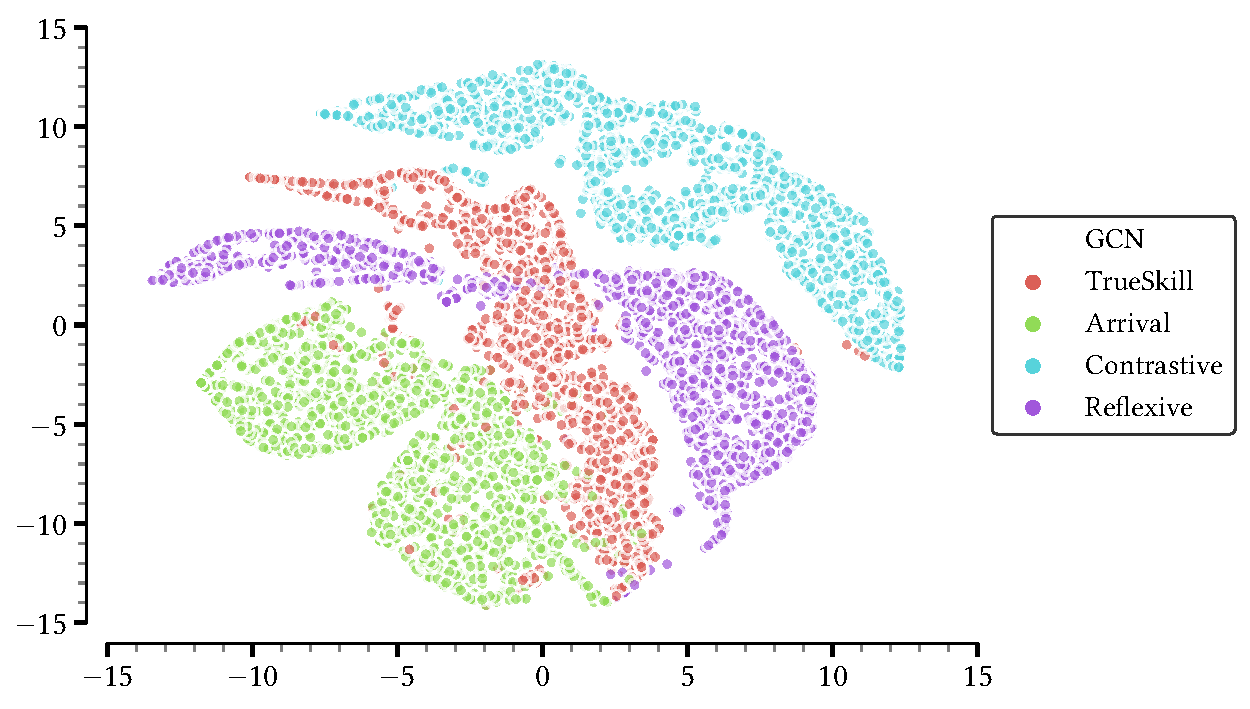
\includegraphics[scale=0.3]{figures/sne_plot.pdf}
  %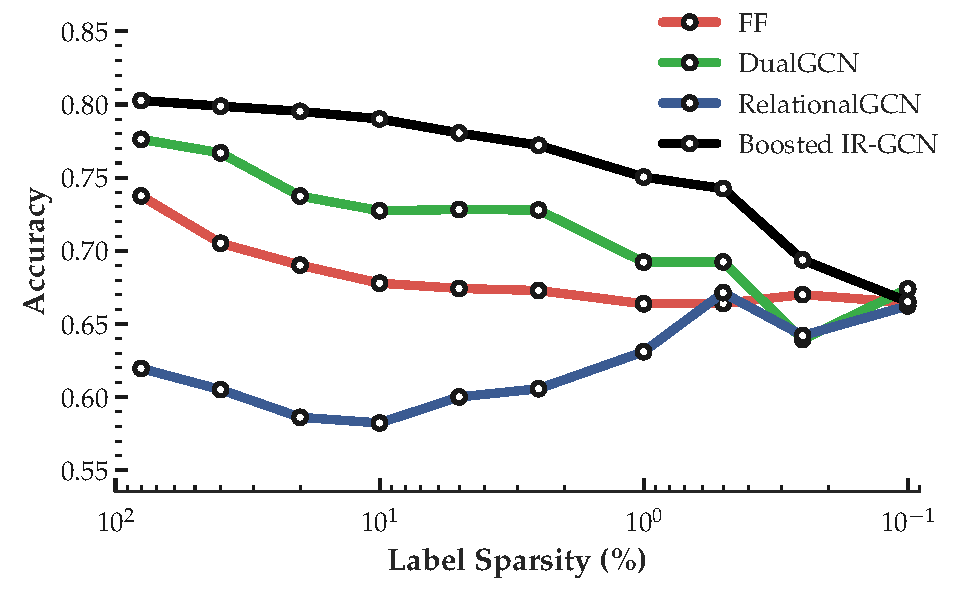
\includegraphics[height=4.2cm,width=0.85\linewidth]{figures/Label_Sparsity}
  %\vspace{-0.15in}
  \caption{\small \label{fig:sne} t-stochastic neighbor embedding (t-SNE) \cite{sne} distributions of the learned vertex representations by our model for Chemistry StackExchange. Each view learns a distinct vertex representation. Best viewed in color.}
  \vspace{-0.1in}
%\end{figure}
\end{wrapfigure}

Among individual views, Contrastive GCN performs best on all the communities. It even beats the best performing baseline DualGCN that uses all the relational views. Note that the contrastive view compares between the candidate answers to a question and uses our proposed contrastive modification to the convolution operation. Arrival Similarity follows Contrastive and then Reflexive. The superior performance of the Arrival Similarity view shows that early answers tend to get accepted and vice versa. It indicates that users primarily use CQA forums for quick answers to their queries. Also, recall that Reflexive predicts each vertex's label independent of other answers to the same question. Thus, the competitive performance of the Reflexive strategy indicates that vertex's features itself are well predictive of the label. TrueSkill Similarity performs at par or slightly worse than Reflexive. \Cref{fig:sne} presents t-SNE distributions \cite{sne} of the learned vertex representations ($\mathbf{Z}_i^K$) of our model applied to Chemistry StackExchange from Science category. Note that each view, including two views under Similarity by Contrast relation, learns a distinct vertex representation. Hence, all views are essential and contribute to our final performance.

Out of the baseline graph ensemble approaches, DualGCN performs significantly better than RelationalGCN by an average of around 26\% for all categories. Recall that in the RelationalGCN model, the convolution output of each view is linearly combined to compute the final output. Linear combination works well for knowledge graphs as each view can be thought of as a feature, and then it accumulates information from each feature. DualGCN is similar to our approach and trains different GCN for each view and later merges their results. However, it enforces similarity in vertex representations learned by each view. This restriction is not suitable for our induced-relationships as they are semantically different (contrastive captures contrast in features vs. similarity enforces label sharing).


%\section{Discussion}
%In this section, we first evaluate importance of each relational view for our boosted model. We then compare with approaches proposed to merge neural networks in general in other domains. Finally, we study robustness of our model to training label sparsity.

%\vspace{-0.1in}
\subsection{Ablation Study on Relation Types}
\begin{table}[h]
  \vspace{-0.0in}
  \small
  %\robustify\bfseries
  \begin{tabular}{l | S[round-mode=places,round-precision=2]@{\hspace{2mm}}|S[round-mode=places,round-precision=2]@{\hspace{2mm}}|S[round-mode=places,round-precision=2]@{\hspace{2mm}}| S[round-mode=places,round-precision=2]@{\hspace{2mm}}|S[round-mode=places,round-precision=2]}
  %\begin{tabular}{l | c | c| c| c|c}
    \toprule
  %  \textbf{Strategies} &
      % \textbf{SF} &
      % \textbf{ENG} &
      % \textbf{SCIFI} &
      % \textbf{PHYS}&
      % \textbf{WP}\\
       \textbf{\{ Relation Type\}} &
        \textbf{Tech} &
        \textbf{Culture} &
        \textbf{Life} &
        \textbf{Sci}&
        \textbf{Business}\\
      \midrule
      C & 71.23 &75.90 &78.71&72.99 & 76.85\\
    \{ TS, AS \} & 67.86 &74.15 &75.75&65.80& 76.13  \\
    R & 68.30 & 73.35 & 76.57 & 67.40 & 75.76 \\
    \{TS, AS \} + R & 69.28 & 75.50 &76.41 &70.11  &77.90 \\
    C + R & 73.04 & 77.66 & 80.25 &73.72 & 80.04 \\
    C + \{ TS, AS \} & 72.81 & 78.04 & 81.41 & 72.19 & 80.15\\
    C + \{ TS, AS \} + R & \bfseries 73.87 & \bfseries 78.74 & \bfseries 81.60&  \bfseries74.68&  \bfseries80.56 \\
    \bottomrule
  \end{tabular}
  \caption{\small \label{tab:relation} 5-fold Accuracy (in \%) comparison for different combination of relation types for our boosted model. Contrastive and Similarity by Contrast relations together performs similar to the final model.}
  \vspace{-0.15in}
\end{table}

We present the results of an ablation study with a different combination of relation types (Contrastive, Similarity, and Reflexive) used for the IR-GCN model in Table \ref{tab:relation}. We conducted this study on the biggest community from each of the five categories, i.e., ServerFault (Technology), English (Culture), Science Fiction (Life), Physics (Science), Workplace (Business).
Similarity by Contrast relation (TrueSkill and Arrival) used in isolation performs the worst among all the variants. Training Contrastive and Similarity by Contrast relation together in our boosted framework performs similar to our final model. Reflexive GCN contributes the least as it does not consider any neighbors.

\vspace{-0.1in}
\subsection{Aggregator Architecture Variants}
\label{sec:agg}
We compare our gradient boosting based aggregation approach with other popular methods used in literature to merge different neural networks discussed in \cref{item:aggregator}.

\begin{table}[h]
  \small
  %\robustify\bfseries
  \vspace{-0.15in}
  \begin{tabular}{l | c | c| c| c|c}
    \toprule
    % \textbf{Method} &
    %   \textbf{SF} &
    %   \textbf{ENG} &
    %   \textbf{SCIFI} &
    %   \textbf{PHYS}&
    %   \textbf{WP}\\
    \textbf{Method} &
     \textbf{Tech} &
     \textbf{Culture} &
     \textbf{Life} &
     \textbf{Sci}&
     \textbf{Business}\\
      \midrule
    Stacking~\cite{Stacking} &68.58 & 74.44 & 79.19 & 70.29 &75.50  \\
    Fusion~\cite{Fusion18}  &72.30 &77.25 & 80.79 & 73.91 &79.01 \\
    NeighborAgg~\cite{graphsage,relationalGCN}  &69.29 &74.28 & 77.94 & 68.42 &78.64   \\
    IR-GCN & \bfseries 73.87 & \bfseries 78.74 & \bfseries 81.60&  \bfseries74.78&  \bfseries80.56 \\
    \bottomrule
  \end{tabular}
  \caption{\small \label{tab:agg} 5-fold Accuracy (in \%) comparison of different aggregator architectures. These architectures perform worse than Contrastive GCN. Fusion performs similarly but is computationally expensive.}
  \vspace{-0.2in}
\end{table}

Table \ref{tab:agg} reports the accuracy results for these aggregator variants as compared to our model. Our method outperforms all the variants with Fusion performing the best. This worse performance reaffirms that existing aggregation models are not suitable for our problem. Note that these approaches perform worse than even Contrastive GCN except Fusion. The fusion approach performs similarly to our approach but is computationally expensive as the input size for each IR-GCN in fusion is linear in the number of all views in the model.

\subsection{Textual Features}
Most of the current literature focuses on using textual features for Answer Selection. In this section, we compare our proposed IR-GCN model to a popular text-based model~\cite{Tan2015}. %proposed for answer selection.

\noindent
\textbf{QA-LSTM/CNN \cite{Tan2015}} uses a stacked bidirectional LSTM model followed by convolution filters to learn embeddings for the question and answer text separately. They then rank answers in decreasing order of the cosine similarity between question and answer embeddings.

  %\item{\textbf{biLSTM+CNN} The basic biLSTM model was extended to learn more composite embedding by using convolution filters on biLSTM output.}
\noindent
\textbf{Textual Similarity (T-GCN)} We create a \textit{Similarity by Contrast} view that connects answers authored by a user where her answer's text is significantly similar (dissimilar) to the question's text than the other competing answers. We used cosine similarity on the learned question and answer embeddings from the QA-LSTM approach as the similarity function.

\noindent
\textbf{IR-GCN + T-GCN} extends our proposed model to also include the Textual Similarity as the third \textit{Similarity by Contrast} view in addition to Arrival and TrueSkill views.
\begin{table}[h]
  \small
  %\robustify\bfseries
  \centering
    \vspace{-0.0in}
  \begin{tabular}{l | S[round-mode=places,round-precision=2]S[round-mode=places,round-precision=2]S[round-mode=places,round-precision=2]S[round-mode=places,round-precision=2]S[round-mode=places,round-precision=2]}
    \toprule
    \textbf{Method} &
      \textbf{Tech} &
      \textbf{Culture} &
      \textbf{Life} &
      \textbf{Sci} &
      \textbf{Business}\\
      \midrule
    QA-LSTM/CNN\cite{Tan2015} & 66.49 & 71.70 & 69.42 & 62.91 & 72.55 \\
    FF~\cite{JendersKN16} & 68.30 & 73.35 & 76.57 & 67.40 & 75.76 \\
    T-GCN & 69.25 & 73.77 & 76.39 & 67.79 & 77.08\\
    IR-GCN & 73.87 & 78.74 & 81.60 & 74.68 & 80.56 \\
    IR-GCN + T-GCN & 73.89 & 78.00  & 81.07 & 74.49 & 78.86\\
    \bottomrule
  \end{tabular}
  \caption{\small \label{tab:text} 5-fold Accuracy comparison of text-based baseline and textual similarity GCN with IR-GCN.}
    \vspace{-0.2in}
\end{table}

In general, the text-based baseline, QA-LSTM, performs worse than even reflexive GCN, as shown in Table \ref{tab:text}. Note that reflexive GCN employs a feedforward model on the activity and user features used in our experiments. This is a surprising result as most of the current literature focus on textual features for the task. Our results indicate that non-textual features are useful too for the answer selection task on StackExchange communities.

Textual Similarity GCN performs better than QA-LSTM and Reflexive GCN. Even though we use the output of QA-LSTM to construct the graph for T-GCN, the graph improves performance as it connects answers across different questions. However, adding the T-GCN view in our proposed IR-GCN model decreases the performance slightly. One possible explanation could be that similarity by contrast views based on user features (Arrival similarity and TrueSkill similarity) are not compatible with views based on textual features.

% \begin{table}[h]
%   \small
%   %\robustify\bfseries
%   \centering
%   \begin{tabular}{l | S[round-mode=places,round-precision=2]S[round-mode=places,round-precision=2]S[round-mode=places,round-precision=2]S[round-mode=places,round-precision=2]S[round-mode=places,round-precision=2]}
%     \toprule
%     \textbf{Method} &
%       \textbf{Tech} &
%       \textbf{Culture} &
%       \textbf{Life} &
%       \textbf{Sci} &
%       \textbf{Business}\\
%       \midrule
%     QA-LSTM/CNN\cite{Tan2015} & 66.49 &  & 69.42 & 62.91 & 72.55 \\
%     FF~\cite{JendersKN16} & 66.00 & 72.22 & 69.85 & 63.63 & 75.57 \\
%     CS-GCN & 66.06 & 72.35 & 71.88 & 64.14 & 75.69 \\
%     IR-GCN & 66.56 & 72.92 & 72.54 & 65.11 & 75.95 \\
%     IR-GCN + CS-GCN & 66.49 & 73.17 & 72.85 & 65.29 & 75.86 \\
%     \bottomrule
%   \end{tabular}
%   \caption{\small \label{tab:textfeature} 5-fold Accuracy comparison of content-based baseline and content-similarity GCN with learnt content embeddings as features in the GCN.}
% \end{table}
%
% We further replaced our activity based features with the learned embeddings obtained after training the QA-LSTM/CNN~\cite{Tan2015} model. We observed that performance of all approaches went down slightly when using content features (Table \ref{tab:textfeature}). As we noted before, GCNs aggregate features among the neighbors. In our similar contrast view, it is not favorable to aggregate content features among the neighbors as we connect answers catering to different questions. Thus, aggregating content features will create noise in the dataset.

\vspace{-0.2in}
\subsection{Discriminative Magnification effect}

% \begin{figure}[tbh]
%   \centering
%   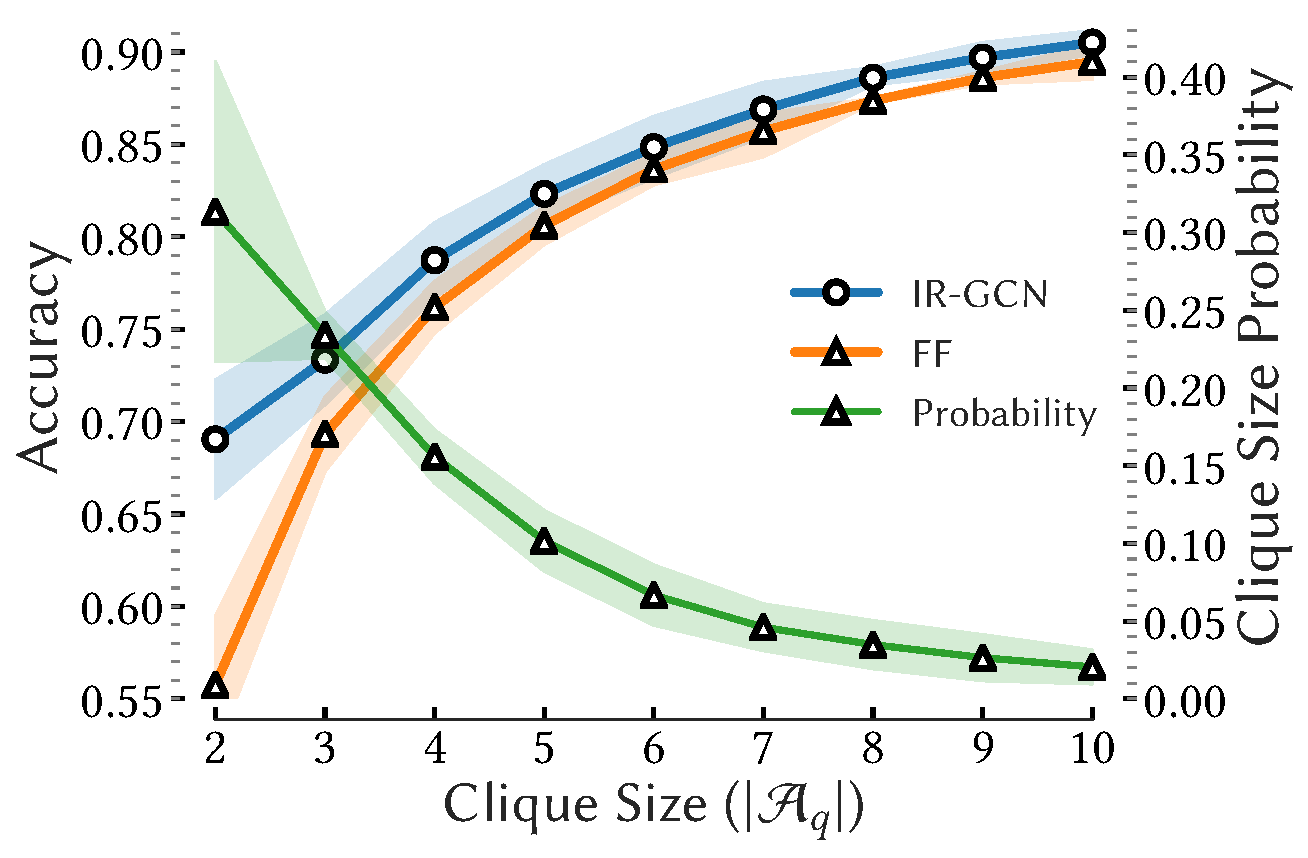
\includegraphics[scale=0.3]{figures/clique_acc.pdf}
%   %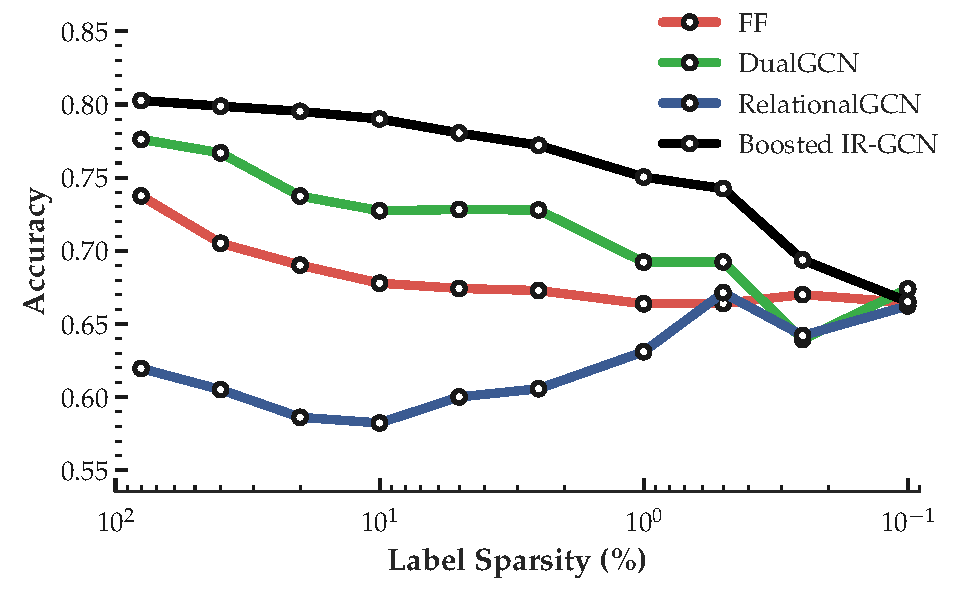
\includegraphics[height=4.2cm,width=0.85\linewidth]{figures/Label_Sparsity}
%   \vspace{-0.12in}
%   \caption{\small \label{fig:clique} Accuracy of our IR-GCN model compared to the FF model with varying clique size (i.e. number of answers to a question, $\vert \mathcal{A}_q \vert$) for Contrastive view . %The results are reported for the largest StackExchange community in all five categories.
% We report averaged results over the largest community of all categories. Our model performs much better for smaller cliques, and the effect diminishes for larger cliques (\cref{eq:contrast}). 80\% of the questions have $< 4$ answers.}
%   \vspace{-0.15in}
% \end{figure}

We show that due to our proposed modification to the convolution operation for contrastive view, we achieve \emph{Discriminative Magnification effect} (\cref{eq:contrast}). Note that the difference is scaled by Clique size ($1 + 1/n-1$), i.e. number of answers to a question, $\vert \mathcal{A}_q \vert$. Figure \ref{fig:clique} shows the accuracy of our IR-GCN model as compared to the FeedForward model with varying clique size. Recall that the FeedForward model predict node labels independent of other nodes and is not affected by clique size. We report average results over the same five communities as above. We can observe that increase in accuracy is much more for lower clique sizes (13\% improvement for $\vert \mathcal{A}_q \vert = 2$ and 4\% for $\vert \mathcal{A}_q \vert = 3$ on average). The results are almost similar for larger clique sizes. In other words, our model significantly outperforms the FeedForward model for questions with fewer candidate answers. However, around 80\% of the questions have very few answers($< 4$), and thus this gain over FF is significant.

\vspace{-0.2in}
\subsection{Label Sparsity}

\begin{figure}[tbh]
  \begin{subfigure}{0.4\textwidth}
    \centering
    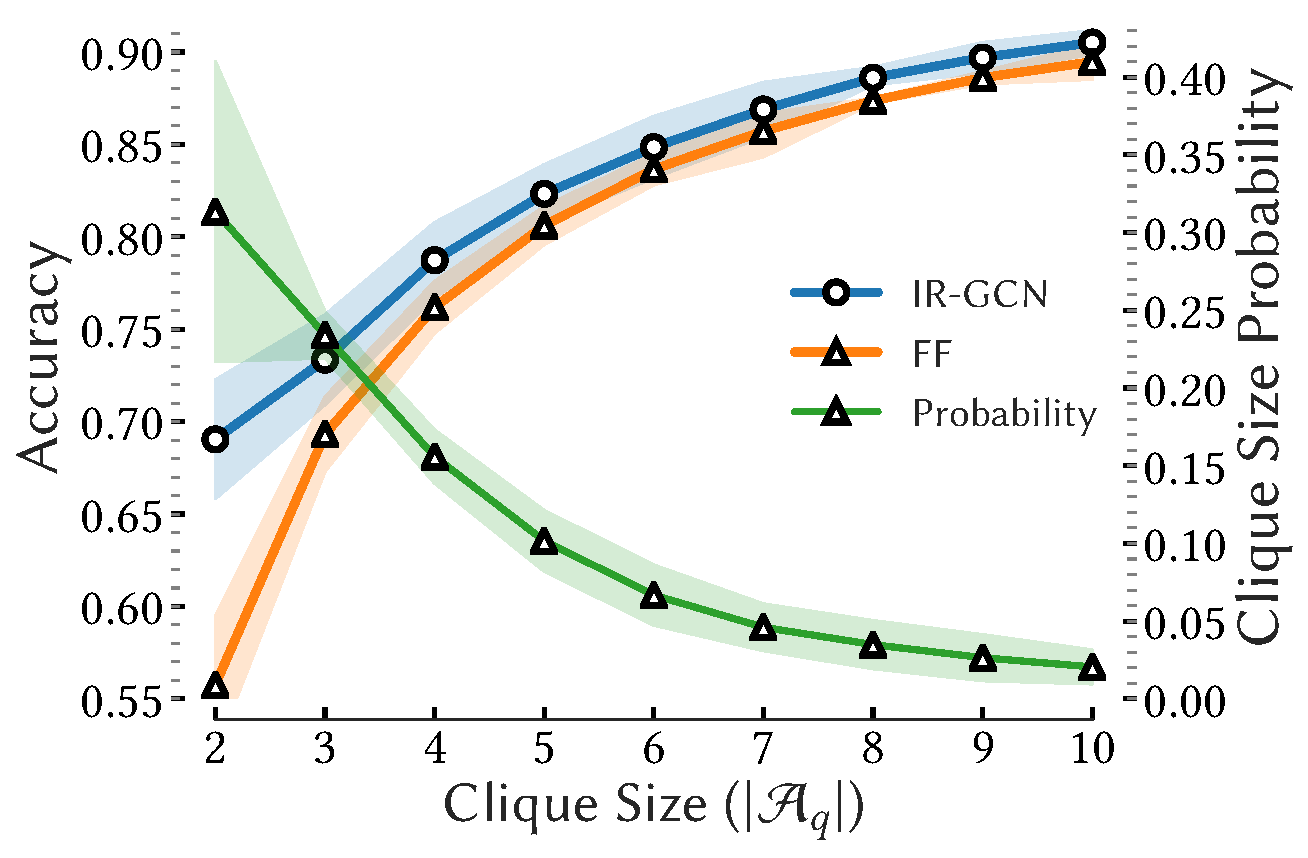
\includegraphics[scale=0.26]{figures/clique_acc.pdf}
    %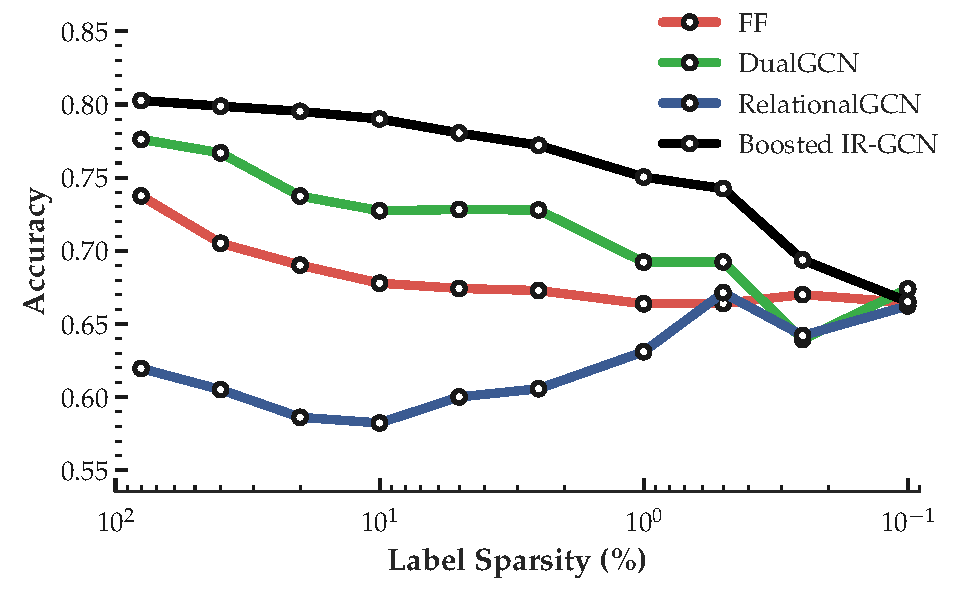
\includegraphics[height=4.2cm,width=0.85\linewidth]{figures/Label_Sparsity}
    \caption{\small \label{fig:clique}}
    %\vspace{-0.12in}
  \end{subfigure} \hspace{0.3in}
  \begin{subfigure}{0.55\textwidth}
      \centering
  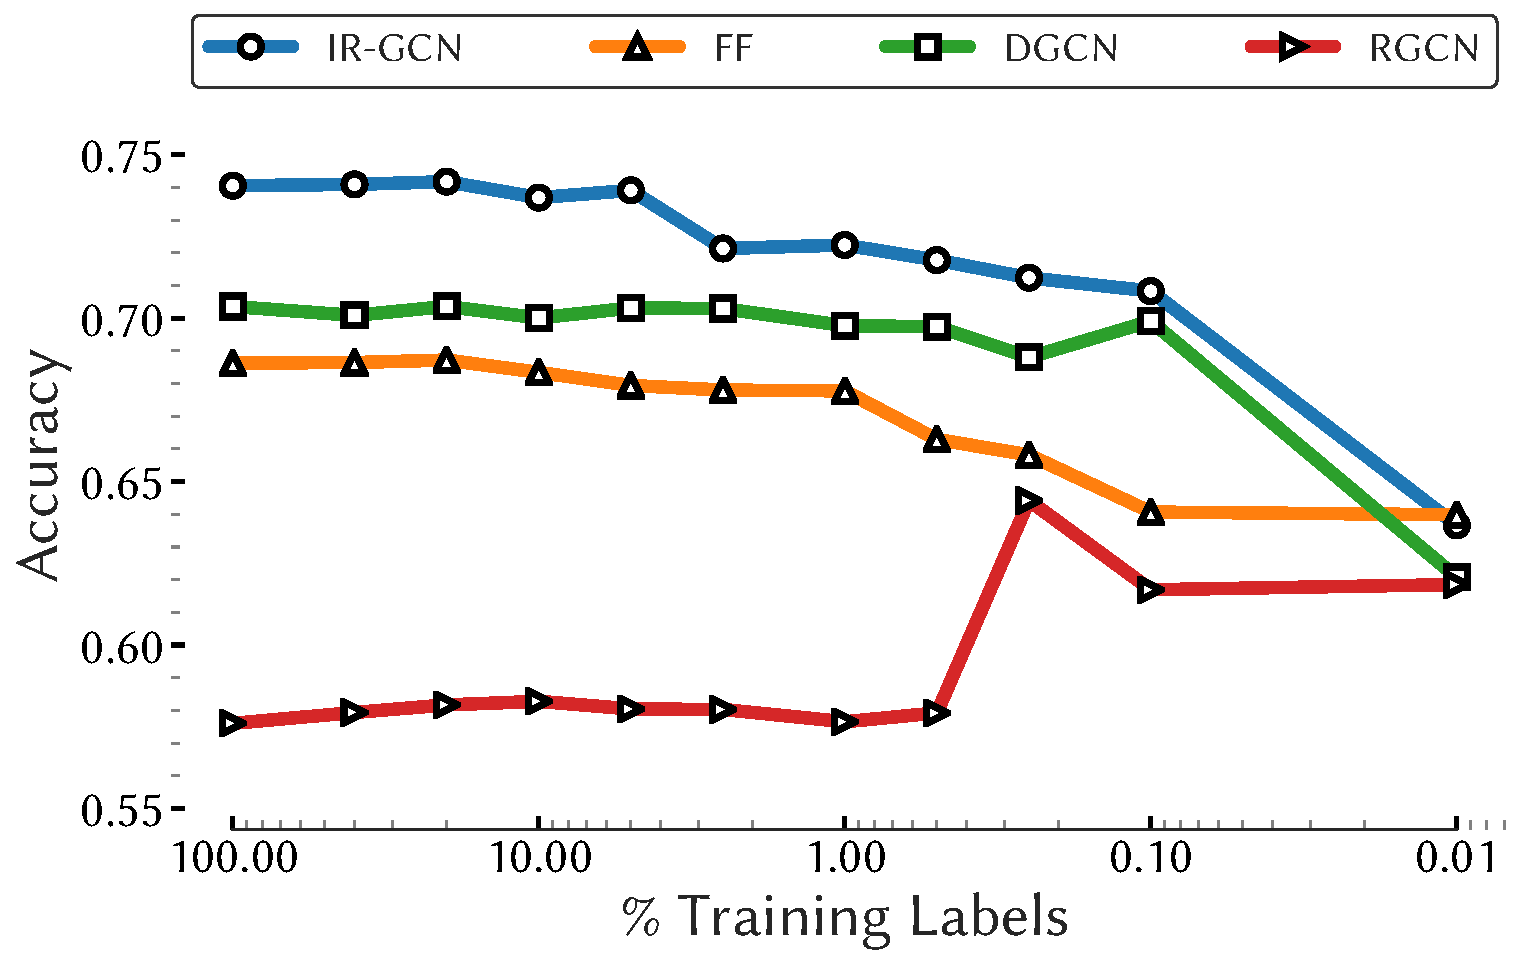
\includegraphics[scale=0.25]{figures/sparsity_acc_physics.pdf}
  %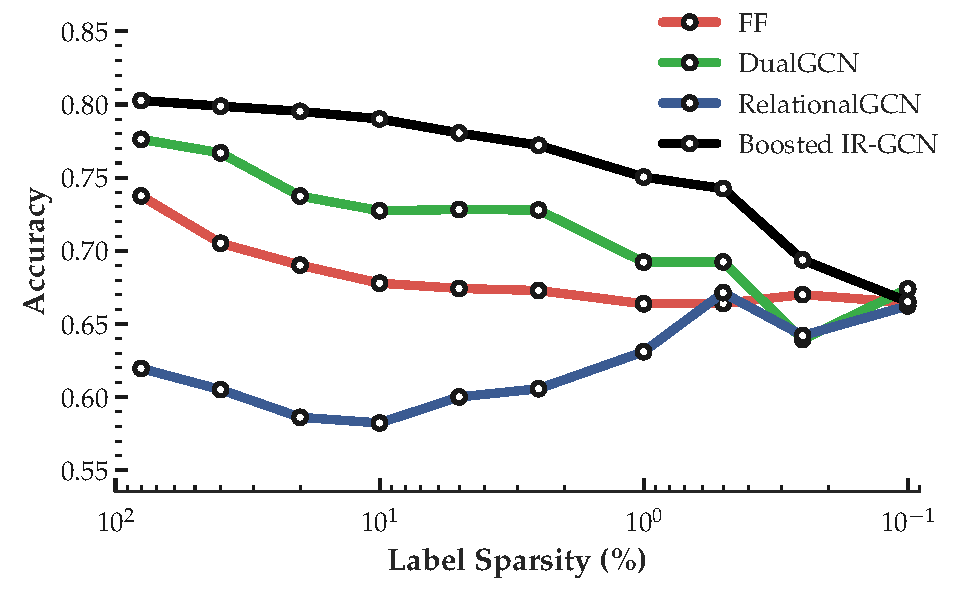
\includegraphics[height=4.2cm,width=0.85\linewidth]{figures/Label_Sparsity}
  %\vspace{-0.2in}
  \caption{\small\label{fig:labelsparsity} }
  \end{subfigure}
  %\vspace{-0.2in}
  \caption{\small a) Accuracy of our IR-GCN model compared to the FF model with varying clique size (i.e., number of answers to a question, $\vert \mathcal{A}_q \vert$) for Contrastive view. %The results are reported for the largest StackExchange community in all five categories.
We report averaged results over the largest community of all categories. Our model performs much better for smaller cliques, and the effect diminishes for larger cliques (\cref{eq:contrast}). 80\% of the questions have $< 4$ answers. \\
b) Change in accuracy with varying training label rates for Physics StackExchange. Our model is more robust to label sparsity than other relation ensemble approaches. RGCN works better with fewer labels as contrastive relation introduces noise in the model. At extreme sparsity, all approaches converge to the same value indicating random selection.
}
\end{figure}
Graph Convolution Networks are robust to label sparsity as they exploit graph structure and are thus heavily used for semi-supervised settings. Figure \ref{fig:labelsparsity} shows the change in accuracy for Physics StackExchange from the Science category at different training label rates. Even though our graph contains disconnected cliques, IR-GCN still preserves robustness to label sparsity.
In contrast, the accuracy of the FeedForward model declines sharply with less label information. Performance of DualGCN remains relatively stable while Relational GCN's performance increases with a decrease in label rate. Relational GCN assumes each view to be of similarity relation, and thus, adding contrastive relation introduces noise in the model. However, as the training labels become extremely sparse, the training noise decreases that leads to a marked improvement in the model. In the case of a meager label rate of 0.01\%, all approaches converge to the same value, which is the expectation of theoretically random selection. We obtained similar results for the other four StackExchange communities but omitted them for brevity.

% \subsection{Change in Accuracy with Clique Size}

\begin{comment}
\subsection{Contrastive GCN Analysis}
\label{ref:analysis}
The ability of neural networks to perform classification in sparse high-dimensional manifolds has been studied in past work, especially in the context of adversarial learning \cite{lu2017safetynet}. We employ the ReLU activation function in our convolution layers and study the outputs of the $k$th layer, i.e. embeddings with k-order locality. This transformation breaks the input space into cells with smooth gradients within each cell, at whose boundaries the piecewise linear function changes (i.e. the likelihood of the two classes of answers).

% In the context of adversarial learning \cite{safetynet} propose the existence of p-domains or cells in the learned manifold, representing a piecewise linear mapping of the transformed features to the class labels. The generalization neutrality property is particularly interesting. Both train and test samples are highly unlikely to lie in p-domains since the number of examples is much smaller than the capacity of the neural network to fit these regions. Weight decay can incentivize relatively small changes in the gradient across these regions resulting in smoother changes.  the ability of the network to fit such regions in the data manifold?

We ask a specific question in the context of our Contrastive IR-GCN. \emph{What is the impact of the layerwise discriminative magnification induced by our formulation?} Discriminative magnifications results in improved separability of the two classes in the later convolving layers, an effect we earlier demonstrated with a sample network in \cref{fig:contrast}. This positively impacts the ability of the model to explain the observed data points (i.e create p-domains that are well aligned with the contrastive samples provided) and improve the generalizability of the learned model to unseen data points. However, it is important to maintain sufficient regularization with weight decay to prevent sparse regions exhibiting sharp gradients which could affect model performance.

The capacity of our model can also be quantified in terms of the VC dimension of the aggregated classifier against the individual learners. Gradient boosting with multiple relation learners (each of which captures a specific aspect of node locality via graph convolution on the induced relations) could boost the capacity of the joint model, enabling better generalization and a more accurate fit in the data manifold (i.e. higher capacity to fit regions to fine distinctions).

Let us denote the upper bound of the VC dimension or capacity of each individual learner as D (If the individual learners do not have identical capacity, the minimum can be used to compute a lower bound on the aggregated learner capacity). Then the gradient boosted learner with T classifiers has a bound on it's capacity~\cite{shalev2014understanding} given by,
\begin{equation*}
\mathcal{VC}_{Agg}  = T \times (D+1) \times(3 \log(T.(D+1))+2)
\label{vcdim}
\vspace{-0.03in}
\end{equation*}

Thus we identify two potential reasons for our performance gains, first the discriminative magnification effect which also supports the strong individual performance of the contrast view, and second the gain in capacity from boosting, which could explain it's advantage over competing aggregation methods.

\end{comment}


\vspace{-0.2in}
\subsection{Limitations} We do recognize certain limitations of our work. First, %we do not deal with content in our model. Our focus in this work is to exploit structural properties between tuples. We believe that adding content will further improve our results. Second, 
we focus on equivalence relations that induce a graph comprising cliques. While cliques are useful graph objects for answer selection, equivalence relations may be too restrictive for other problems (e.g., the relation is not transitive). However, our modular framework does apply to arbitrary graphs, except that~\Cref{eq:restrictk} will no longer be an \emph{exact} convolution but be an approximation. Second, we assume no evolution in author skills. This assumption is not true as users evolve with experience. We aim to address this in future work.



%First, creating induced links require domain knowledge or empirical analysis of the dataset. Second, we do not exploit the content in our model. Although we achieve significant improvements with a basic feature set, the content could be helpful in semi-supervised settings. Third, we assume no evolution in author skills. This assumption is not true as users evolve with experience. We aim to address this in future work.
%\vspace{5pt}




%Our model showed significant gains over state-of-the-art baselines for combining information from semantically different relational links in a graph. Our model is also more robust to training label sparsity as compared to other aggregator GCN approaches. We reasoned that the performance gains achieved by our aggregation strategy can be attributed in part to the enhanced learning capacity of the boosted model and the effect of discriminative feature magnification. Finally, we presented a few limitations and possible future extensions.




%\textbf{Observation 1} - Inducing p-domains in the learned manifold to separate classes\\\\
%In this explanation, we assume the graph convolutional network uses ReLU and weight decay because they are representative, make it easier to explain, and likely to extend to other conditions with some modifications. We have a network with N layers of ReLU's and study the values at the output of the $k$th layer of ReLUs (k-order locality). This is a piecewise linear function of x. Such functions break up the input space into cells, at whose boundaries the piecewise linear function changes (i.e., the likelihood of the two classes of answers). Now assume that for some class y (+ or -1) there exist p-domains (union of cells) D in the input space such that: (a) there are no or few examples in the p-domain; (b) the measure of D under P(X) is small; (c) The probability of a specific class (either + or -1) is large inside D and small outside D. We will use the term "p-domain" to refer to domains with these properties, inspired by past work \cite{safetynet}. The notion of p-domains has been used to study the discontinuities introduced by neural network based classifiers in high dimensional spaces \cite{safetynet}.
%
%
%\textbf{How does discriminative magnification impact the p-domains induced by the graph convolutional learner?\\}
%Generalization-neutral: The requirement that p-domains have small measure in P(X) means that both train and test examples are highly unlikely to lie in p-domains (given the high dimensionality of the induced space as well as the relatively small number of training samples). A system with p-domains could thus generalize well to new unseen examples. Note that the discriminative magnification effect achieved in subsequent convolutional layers positively impacts the ability of the model to explain the observed data points (i.e create p-domains that are well aligned with the contrastive samples provided). This in turn is likely to improve the generalizability of the learned model to unseen data points, and could hence explain the strong performance observed with the contrast learner.
%
%
%\textbf{Observation 2} - Gradient boosting can further amplify the ability of neural networks to exploit discriminative magnification \\\\
%$$Add VC dimension equation here$$
%\end{comment}

\section{Related Work}
\label{sec:related}
Our work intersects two research areas; Answer Selection and handling multi-relational social data, primarily via Graph Convolution.

\noindent
\textbf{Answer Selection}
In CQA forums, previous answer selection literature includes feature-driven models and deep text models.
%They either choose the best one from the candidate pool \cite{BurelMA16, TianZL13, JendersKN16, TianL16, CalefatoLN16} or carefully pick several good answers \cite{ZhangLSW17, WuWS18, ShaZQCS18, WenMFZ18, NieWZWGY17, GuoYXYW17, WangL016, WangN15}.

\noindent
\emph{Feature-Driven Models} in CQA identify and incorporate user features, content features, and thread features, e.g., in tree-based models to identify the best answer. Tian et al. \cite{TianZL13} found that the best answer tends to be early and novel, with more details and comments. Jenders et al. \cite{JendersKN16} trained classifiers for online forums, Burel et al. \cite{BurelMA16} emphasize the Q\&A thread structure.  %Feature-driven models \cite{BurelMA16} develop features from three different perspectives: 1) \emph{User features} from questioner and answerer; 2) \emph{Content features} from question and answer itself; 3) \emph{Thread features} from the relationship within one answer pool.


% Feature-driven models \cite{BurelMA16} develop features from three different perspectives: user features, content features, and thread features.
% These features are fed into classifiers, such as tree-based models \cite{BurelMA16, JendersKN16, TianZL13} to identify the best answer. \citet{TianZL13} found that the best answer is usually the earlier and most different one, and tends to have more details and comments. \citet{JendersKN16} trained several classifiers for online MOOC forums. Different from existing works, \citet{BurelMA16} emphasize on the thread-like structure of Q\&A and introduce four thread-based normalization methods. These models predict the answer label independently of the other answers for the question.


\noindent
\emph{Deep Text Models} learn optimal QA text-pair representations to select the best answer \cite{ZhangLSW17,WuWS18,WangN15}. Feng et al. \cite{FengXGWZ15} augment CNNs with discontinuous convolution for improved representations; Wang et al. \cite{Tan2015} use stacked biLSTMs to match question-answer semantics.
%\citet{SukhbaatarSWF15} use attention mechanism in an end-to-end memory framework.




%Other later works also use attention networks, such as the hybrid attention model \cite{WenMFZ18}, multi-view attention model \cite{ShaZQCS18}, and interactive attention model \cite{ZhangLSW17}. According to a newest survey \cite{LaiBL18}, deep text models can be classified into three groups based on the structure: Siamese Architecture \cite{FengXGWZ15}, Attentive Architecture \cite{WenMFZ18, ShaZQCS18, ZhangLSW17} and Compare-Aggregate Architecture \cite{Bian0YCL17, TranLHZBB18}.

\noindent
\textbf{Graph Convolution} is applied in spatial and spectral domains to compute graph node representations for downstream tasks including node classification \cite{gcn}, link prediction \cite{relationalGCN}, multi-relational tasks~\cite{rase} etc. Spatial approaches employ random walks or k-hop neighborhoods to compute node representations \cite{DeepWalk,node2vec,LINE} while fast localized convolutions are applied in the spectral domain\cite{deferrard,duvenaund}. Our work is inspired by Graph Convolution Networks (GCN) \cite{gcn}, which outperforms spatial convolutions and scales to large graphs. GCN extensions have been proposed for signed networks \cite{signedgcn}, inductive settings \cite{graphsage}, multiple relations \cite{DualGCN,relationalGCN} and diffusion~\cite{infvae}. However, GCN variants assume label sharing, which cannot model contrastive relations in our setting.

% Recent approaches learn multiple GCNs for higher powers of the adjacency matrix and motifs \cite{NGCN, MotifGCN}, but do not apply to our setting as we model disconnected cliques.
\noindent
\textbf{Multi-Relational Modeling: } While text and feature models treat answer content independently, we focus on integrating multi-relational aspects in the prediction. We identify a few related threads; adversarial approaches to integrate social neighbor data~\cite{adv_social,adv_neighbor}; meta-learning to adapt across data modalities or tasks~\cite{maml}. Different from these directions, we focus on the flexibility and simplicity of our multi-relational graph formulation for modeling user-generated content.

\section{Conclusion}
\label{sec:conclusion}
% We proposed a Graph Convolution based model to solve Answer selection for Community Question Answer platforms. We introduced data induced relationships to capture interaction between different qa pairs in the dataset. Contrastive relation captured difference between an answer and other answers for a question, contrastive similarity linked answers which are significantly different from other answers in skill rating of their answerers or arrival time. Reflexive relationship was introduced to exploit features of the answer itself. We proposed an adaboost based ensemble method to accumulate weak signals from each induced relationship. We also beat state-of-the-art baselines for graph ensemble and answer selection for Reddit and StackExchange.
% Future work can include exploiting text information to improve prediction or extending our model for semi supervised settings with minimal label supervision.

This paper addressed the question of identifying the accepted answer to a question in CQA forums. We developed a novel induced relational graph convolutional (IR-GCN) framework to address this question. We made three contributions. First, we introduced a novel idea of using strategies to induce different views on $(q,a)$ tuples in CQA forums. Each view consists of cliques and encodes---reflexive, similar, contrastive---relation types. Second, we encoded label sharing and label contrast mechanisms within each clique through a GCN architecture.  Our novel contrastive architecture achieves \emph{Discriminative Magnification} between nodes. Finally, we show through extensive empirical results on StackExchange that boosting techniques improved learning in our convolutional model.
%This was a surprising result since much of the work on neural architecture focuses on stacking, fusion or aggregator architectures.
%We conduct extensive experiments with excellent experimental results over the state-of-the-art baselines for 50 communities on StackExchange.
Our ablation studies show that the contrastive relation is most effective individually in StackExchange. 
%As part of future work, we plan to fold the evolution of players' skills into our model.
%include content into the convolutional framework.
%fold into our model evolution of players skill and .


%\RequirePackage{fix-cm}
%
%\documentclass{svjour3}                     % onecolumn (standard format)
\documentclass[smallcondensed]{svjour3}     % onecolumn (ditto)
%\documentclass[smallextended]{svjour3}       % onecolumn (second format)
%\documentclass[twocolumn]{svjour3}          % twocolumn
%
\smartqed  % flush right qed marks, e.g. at end of proof
%
%
\makeatletter
%\def\cl@chapter{\cl@chapter \@elt {theorem}}%bug in class
\def\cl@chapter{\@elt {theorem}}
\makeatother
%
\usepackage{times}  % DO NOT CHANGE THIS
\usepackage{helvet} % DO NOT CHANGE THIS
\usepackage{courier}  % DO NOT CHANGE THIS
\usepackage[hyphens]{url}  % DO NOT CHANGE THIS
\usepackage{graphicx} % DO NOT CHANGE THIS
\urlstyle{rm} % DO NOT CHANGE THIS
\def\UrlFont{\rm}  % DO NOT CHANGE THIS
\frenchspacing  % DO NOT CHANGE THIS
\setlength{\pdfpagewidth}{8.5in}  % DO NOT CHANGE THIS
\setlength{\pdfpageheight}{11in}  % DO NOT CHANGE THIS

\usepackage{latexsym}
\usepackage{amsmath}
\usepackage{amssymb}
\usepackage{subcaption}
\captionsetup{compatibility=false}
%\usepackage{caption}
\usepackage{cleveref}
\usepackage[normalem]{ulem}
\usepackage{array}
\usepackage{multirow}
\usepackage{booktabs} % For formal tables

\begin{document}

%\section{Appendix}
\section{Section 3.1.3 : Similarity by Contrast}
The exact view construction algorithm for similarity by contrast views are:

\textbf{TrueSkill Similarity} connects answers authored by a specific user, where the difference in his skill over peers is greater than margin $\delta$. Specifically, if the user authors answers $a, a'$ to questions $q, q'$, we create a link between $a$ and $a'$ if %$\lvert S_{u,a} - S_{u, b} \rvert > \delta; \forall b \in \mathcal{A}_(q)$ and $\lvert S_{u,a'} - S_{u, c} \rvert > \delta; \forall c \in \mathcal{A}_(q')$
\begin{align*}
 \lvert S_{u,a} - S_{u, b} \rvert &> \delta; \forall b \in \mathcal{A}_(q) \\
 \lvert S_{u,a'} - S_{u, c} \rvert &> \delta; \forall c \in \mathcal{A}_(q')
\end{align*}
where $S_{u,a}$ is the skill value for the user who authored answer $a$. Similarly, a link is created for the opposite case when difference is less than $-\delta$.
% \begin{align*}
% \lvert S_{u,a} - S_{u, b} \rvert < -\delta; \forall b \in \mathcal{A}(q) \\
% \lvert S_{u,a'} - S_{u, c} \rvert < -\delta; \forall c \in \mathcal{A}(q')
% \end{align*}

We estimate the user skill values with the TrueSkill rating system (\url{https://pypi.org/project/trueskill/}) computed with their historic performance in the community. TrueSkill values are normally distributed among users (\cref{fig:clique}).

% developed by Microsoft Reasearch for ranking and matching similar skill game players for Xbox Live. In our settings, each question is a multi player game with all answerers as game players. The user who gives credible answer is the winner. True Skill rating then computes player's skill through bayesian inference on the basis of credibility label of his answered questions. The estimated ratings are a Gaussian distribution where $\mu$ denotes the average skill of the player. We use the mean value as skill value for our computations.


\begin{figure}[th]
  \centering
  \begin{subfigure}{0.5\textwidth}
    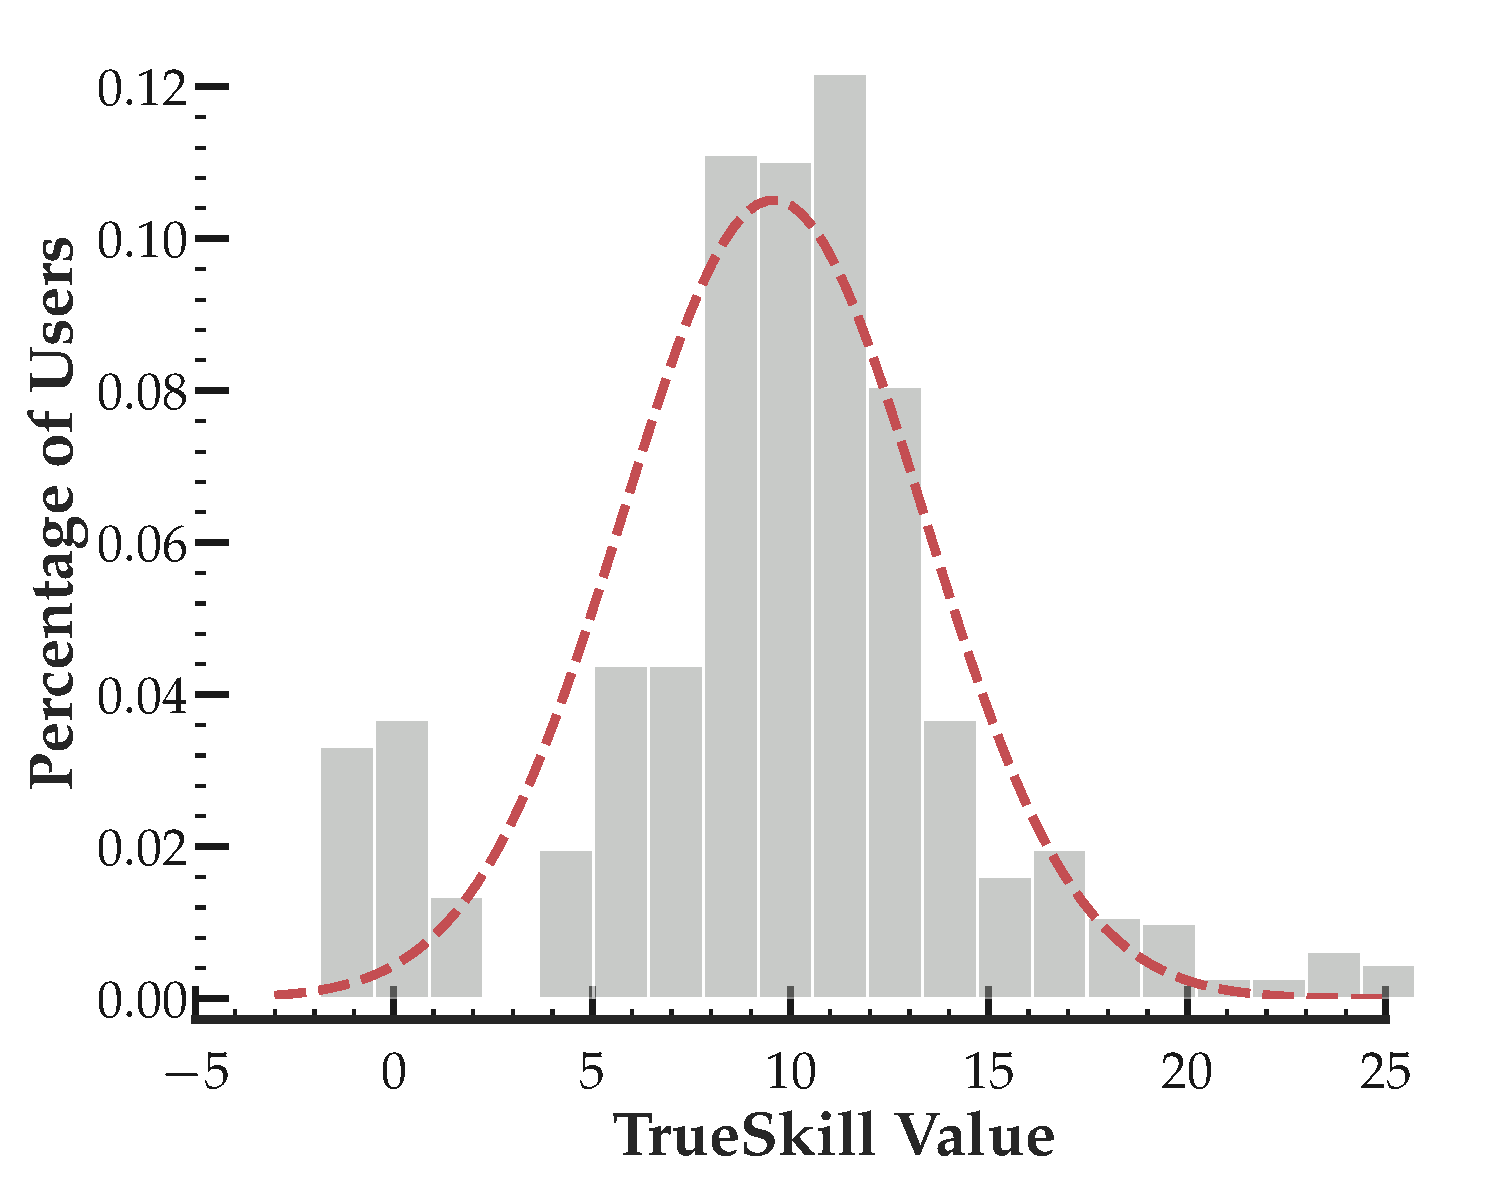
\includegraphics[scale=0.25]{figures/TrueSkill}
    \caption{TrueSkill Distribution}
  \end{subfigure}%
  \begin{subfigure}{0.5\textwidth}
    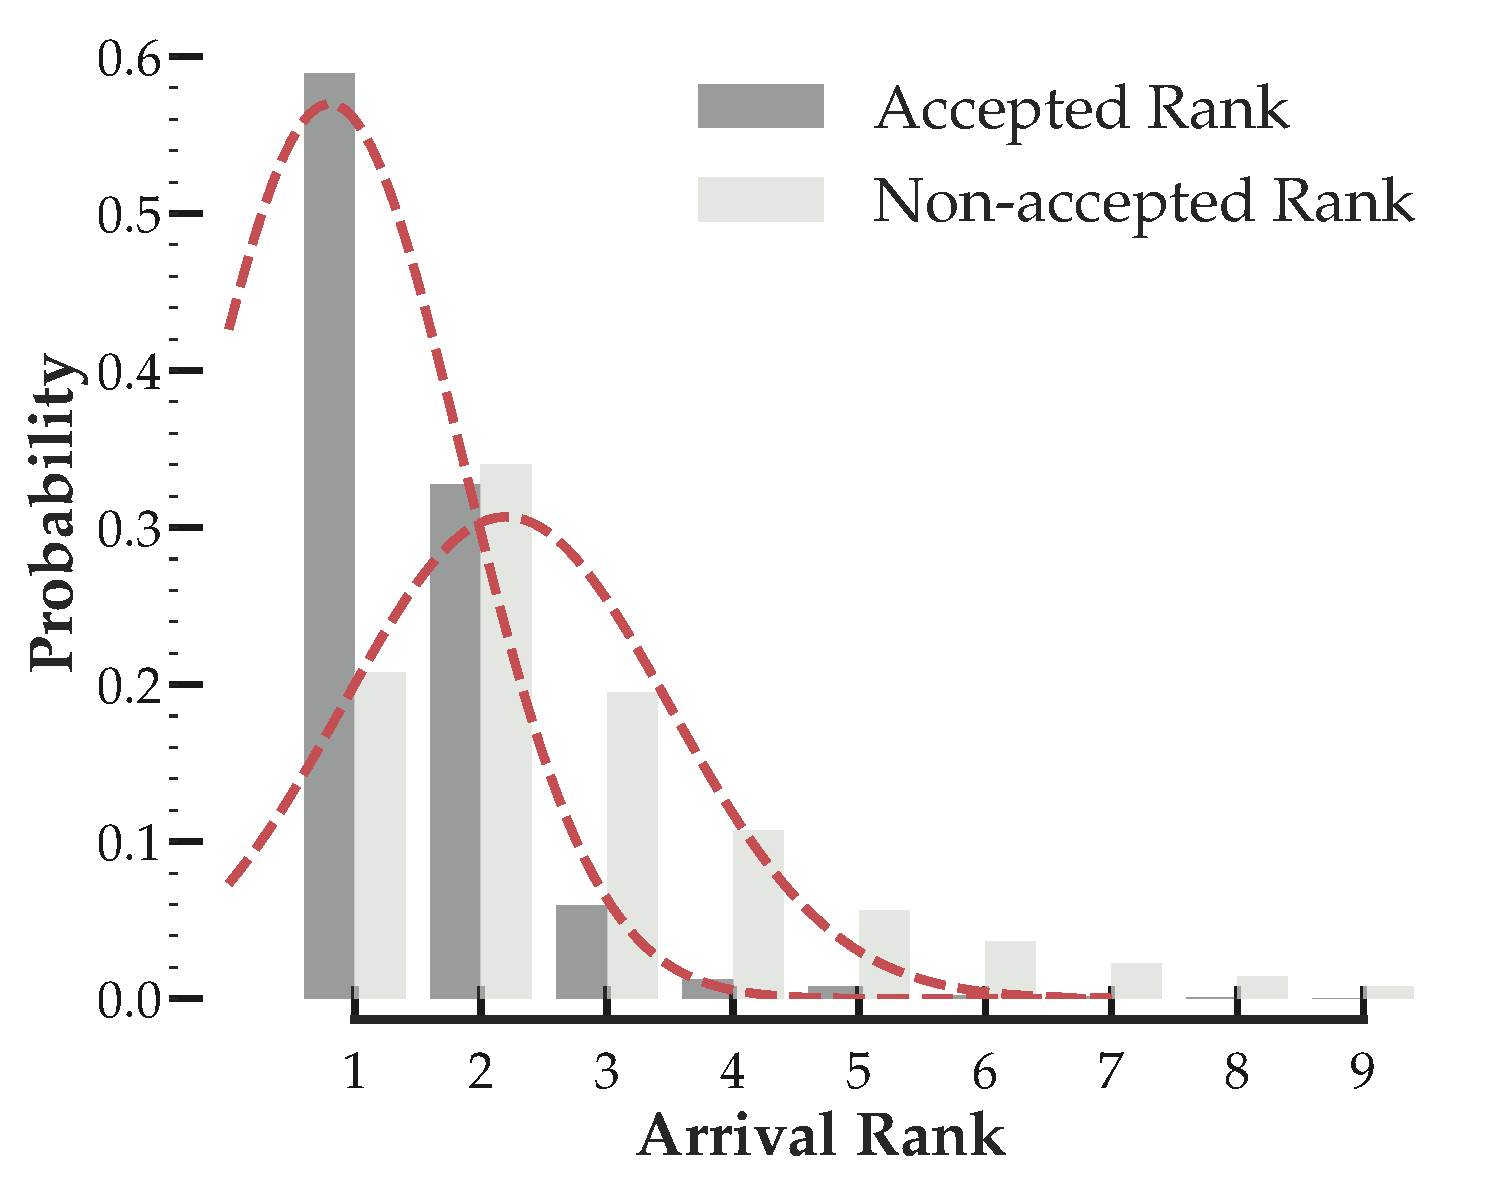
\includegraphics[scale=0.25]{figures/ArrivalRank}
    \caption{ArrivalRank Distribution}
  \end{subfigure}
  \caption{\label{fig:clique} Distribution of the TrueSkill values of users and ArrivalRank of accepted answers and non-accepted answers for the movie StackExchange. Early answers are more likely to be accepted and variance of TrueSkill similarity across users is high.}
\end{figure}

\textbf{Arrival Similarity}
The temporal arrival patterns of answers are correlated to their acceptance probabilities (\cref{fig:clique}). For a specific user authoring answers $a, a'$ to questions $q, q'$, we establish a link between these answers if %$\lvert T_{a} - T_{b} \rvert > \gamma \times \max(T_{b}); \forall b \in \mathcal{A}_(q)$ and $\lvert T_{a'} - T_{c} \rvert > \gamma \times \max(T_{c}); \forall c \in \mathcal{A}_(q')$.
%Highly skilled/active users tend to follow consistent patterns in when they author answers, relative to the other competing answers.
%We observe that earlier posted answers have a higher chance of acceptance in CQA platform as shown in Figure \ref{fig:clique}. Therefore,
\begin{align*}
 \lvert T_{a} - T_{b} \rvert &> \gamma \times \max(T_{b}); \forall b \in \mathcal{A}_(q) \\
 \lvert T_{a'} - T_{c} \rvert &> \gamma \times \max(T_{c}); \forall c \in \mathcal{A}_(q')
\end{align*}
where $T_{a}$ represents the relative time-gap between answer $a$ and the question $q$. Conversely, we create links when difference is less than $-\gamma \times \max(T_{b})$.
%\begin{align*}
% \lvert T_{a} - T_{b} \rvert < -\gamma * max(T_{b}); \forall b \in \mathcal{A}(q) \\
% \lvert T_{a'} - T_{c} \rvert < -\gamma * max(T_{c}); \forall c \in \mathcal{A}(q')
%\end{align*}
Our hypotheis is that a similar answering schedule indicates similar user confidence or skill across questions.

\section{Section 4.2 : Contrastive Convolution}
\label{ref:analysis}
In this section, we provide a theoretical analysis of our contrastive convolution.
The ability of neural networks to perform classification in sparse high-dimensional manifolds has been studied in past work, especially in the context of adversarial learning \cite{lu2017safetynet}. We employ the ReLU activation function in our convolution layers and study the outputs of the $k$th layer, i.e. embeddings with k-order locality. This transformation breaks the input space into cells with smooth gradients within each cell, at whose boundaries the piecewise linear function changes (i.e. the likelihood of the two classes of answers).

% In the context of adversarial learning \cite{safetynet} propose the existence of p-domains or cells in the learned manifold, representing a piecewise linear mapping of the transformed features to the class labels. The generalization neutrality property is particularly interesting. Both train and test samples are highly unlikely to lie in p-domains since the number of examples is much smaller than the capacity of the neural network to fit these regions. Weight decay can incentivize relatively small changes in the gradient across these regions resulting in smoother changes.  the ability of the network to fit such regions in the data manifold?

We ask a specific question in the context of our Contrastive IR-GCN. \emph{What is the impact of the layerwise discriminative magnification induced by our formulation?} Discriminative magnifications results in improved separability of the two classes in the later convolving layers, an effect we earlier demonstrated with a sample network in \cref{fig:contrast}. This positively impacts the ability of the model to explain the observed data points (i.e create p-domains that are well aligned with the contrastive samples provided) and improve the generalizability of the learned model to unseen data points. However, it is important to maintain sufficient regularization with weight decay to prevent sparse regions exhibiting sharp gradients which could affect model performance.

The capacity of our model can also be quantified in terms of the VC dimension of the aggregated classifier against the individual learners. Gradient boosting with multiple relation learners (each of which captures a specific aspect of node locality via graph convolution on the induced relations) could boost the capacity of the joint model, enabling better generalization and a more accurate fit in the data manifold (i.e. higher capacity to fit regions to fine distinctions).

Let us denote the upper bound of the VC dimension or capacity of each individual learner as D (If the individual learners do not have identical capacity, the minimum can be used to compute a lower bound on the aggregated learner capacity). Then the gradient boosted learner with T classifiers has a bound on it's capacity~\cite{shalev2014understanding} given by,
\begin{equation*}
\mathcal{VC}_{Agg}  = T \times (D+1) \times(3 \log(T.(D+1))+2)
\label{vcdim}
\vspace{-0.03in}
\end{equation*}

Thus we identify two potential reasons for our performance gains, first the discriminative magnification effect which also supports the strong individual performance of the contrast view, and second the gain in capacity from boosting, which could explain it's advantage over competing aggregation methods.

\section{Section 5 : Aggregating Induced Views}
The prior aggregation methods used in the literature were adapted for our GCN model as follows:

\textbf{Neighborhood Aggregation:} is a multi relational approach that aggregates neighbors of the nodes from all views. Thus, the final adjacency matrix is the sum of all the individual adjacency matrices of each view, i.e., $A = \sum_{S_i \in \mathbf{S}} A_i$. We, then, apply Graph Convolution Network to this updated Adjacency matrix.

\textbf{Stacking:} stacks all GCNs belonging to a view such that output of a lower GCN is fed as an input to the GCN directly above it. Thus, output from the last layer of GCN for view $i$, $Z_i^K$ s.t. $  S_i \in \textbf{S}$ will act as input features, $Z_j^0$ for some other view $j$ s.t. $S_j \in \{\textbf{S}-S_i \}$ if view $j$ is directly above the view $i$. In our experiments, we obtain the best performance by using the following order: Contrastive, Similarity by Contrast followed by Reflexive.

\textbf{Fusion:} treats each GCN as a separate model and appends the output from the final layer of each GCN i.e. $Z_i^K; \forall S_i \in \textbf{S}$ to the input of all the other GCN's, i.e. $Z_j^0 \forall S_j \in \textbf{S}-S_i$ along with the original features. Thus, the input of each GCN is linear in $\vert \textbf{S} \vert$.

\section{Section 6.1 : Dataset}
The list of 50 StackExchange communities per category are;
\begin{itemize}
\item Technology: AskUbuntu, Server Fault, Unix, TEX, Electronics, Gis, Apple, Wordpress, Drupal, DBA

\item Culture/Recreation: English, Travel, RPG, Judaism, Puzzling, Bicycles, German, Christianity, BoardGames, History

\item Life/Arts: Scifi, DIY, Academia, Graphic Design, Money, Photo, WorldBuilding, Movies, Music, Law

\item Science: Stat, Physics, MathOverflow, CS, Chemistry, Biology, Philosophy, CS Theory, Economics, Astronomy

\item Professional/Business: Workplace, Aviation, Writers, Open source, Freelancing, CS Educators, Quant, PM, Parenting
\end{itemize}

\section{Section 6.2.1 : Baselines }
\textbf{Dual GCN (DGCN)} The mean squared error (MSE) between vertex representations of two views is defined as, for instance,
\begin{equation*}
 \mathcal L_{reg}(Z_c, Z_{ts}) = \frac{1}{n} \sum_{j \in {1,n}}  \lVert Z_c^j - Z_{ts}^j \lVert
\end{equation*}
computes the MSE loss between Contrastive and TrueSkill Similarity GCN.
\cite{DualGCN} proposed the model for two GCN representations.
We extend the original two GCN model \cite{DualGCN} to four GCN, each representing our relational views between the nodes. We minimize the supervised loss with respect to the best performing GCN model (Contrastive), and its node representation's alignment with respect to all other GCN's node representations.
The Contrastive view is seen to exhibit the best performance in isolation. Thus, the DualGCN loss can be given by:
\begin{equation*}
  %\mathcal L  = \mathcal L_0(Z_c) + \lambda{(t)} \left( \mathcal L_{reg}(Z_c, Z_{ts}) + \mathcal L_{reg}(Z_c, Z_{as}) + \mathcal L_{reg}(Z_c, Z_r) \right)
  \mathcal L  = \mathcal L_0 +  \lambda{(t)} \left( \sum_{S_i \in \mathbf{S}, S_i \neq c} \lVert \mathbf{Z}_c^K - \mathbf{Z}_i^K \lVert \right)
\end{equation*}
where $\mathcal L_0$ represents the supervised loss and $\mathbf{Z}_c^K$ is the node representations of the Contrastive GCN.

\noindent
\textbf{Relational GCN (RGCN)} \cite{relationalGCN} combines the output representations of previous layer of each view $\mathbf{Z}_i^{k-1}$ of layer $k-1$ of each view to compute an aggregated input to layer $k$.
Formally,
\begin{equation*}
  \mathbf{Z}_{rgcn}^{k} = \sigma \left( \sum_{S_i \in \mathbf{S}} \mathbf{Z}_i^{k-1}\right)
\end{equation*}
where $Z_{rgcn}$ is final output of this model at layer $k$ and $\sigma$ is the activation function.

\section{Section 6.3 : Performance Analysis}
The breakdown of the results by the StackExchange community are given in the tables below.(Technology: \cref{tab:stackacc}, Culture: \cref{tab:stackacc2}, Life: \cref{tab:stackacc3}, Science: \cref{tab:stackacc4}, Business: \cref{tab:stackacc5}).
\begin{table*}[h]
  %\robustify\bfseries
  %\small
  \centering
    %\setlength{\tabcolsep}{0.5pt}
 %\begin{tabular}{l|S[round-mode=places,round-precision=2]@{\hspace{1mm}}S@{\hspace{1mm}}|S[round-mode=places,round-precision=2]@{\hspace{1mm}}S@{\hspace{1mm}}|S[round-mode=places,round-precision=2]@{\hspace{1mm}}S@{\hspace{1mm}}|S[round-mode=places,round-precision=2]@{\hspace{1mm}}S@{\hspace{1mm}}|S[round-mode=places,round-precision=2]@{\hspace{1mm}}S@{\hspace{1mm}}S[round-mode=places,round-precision=2]@{\hspace{1mm}}S@{\hspace{1mm}}}
 %\begin{tabular}{l|S[round-mode=places,round-precision=2]S|S[round-mode=places,round-precision=2]S|S[round-mode=places,round-precision=2]S|S[round-mode=places,round-precision=2]S|S[round-mode=places,round-precision=2]SS[round-mode=places,round-precision=2]S}
 %\resizebox{1.5\columnwidth}{!}{
 \begin{subtable}{\textwidth}
  \begin{tabular}{l|c c|c c|c c|c c|c c}
     \toprule
     \multirow{2}{*}{Method} &
        \multicolumn{2}{c}{\textbf{AskUbuntu}} &
       \multicolumn{2}{c}{\textbf{Serverfault}} &
       \multicolumn{2}{c}{\textbf{Unix}} &
       \multicolumn{2}{c}{\textbf{TEX}} &
       \multicolumn{2}{c}{\textbf{Electronics}}\\
       &{Acc(\%)} & {MRR}&{Acc(\%)} & {MRR}&{Acc(\%)}& {MRR}&{Acc(\%)} & {MRR}&{Acc(\%)} & {MRR}\\
       %\cmidrule(lr){1-1}\cmidrule(lr){2-21}%\cmidrule(lr){12-21}
       \midrule
     \textbf{RF~\cite{BurelMA16,TianZL13}} & 64.63 & 0.668 & 68.38 & 0.648 & 70.90 & 0.597 & 64.93 & 0.717 & 67.69 & 0.699\\


     \textbf{FF~\cite{JendersKN16}} & 68.49 & 0.789 & 68.29 & 0.769 & 73.14 & 0.730 & 65.43 & 0.795 & 68.26 & 0.797\\
     %biLSTM & 63.84 & 0.6887 & 64.40 & 0.6772 & 70.65 & 0.5679 & 58.27 & 0.6944 & 58.10 & 0.6939 & 64.31 & 0.5869 \\
     %biLSTM+CNN & 67.86 & 0.7115 & 68.95 & 0.7009 & 73.08 & 0.6253 & 61.15 & 0.7050 & 59.15 & 0.7279 & 66.75 & 0.5997 \\
     \textbf{DGCN~\cite{DualGCN}} & 70.25 & 0.794 & 72.01 & 0.768 & 75.16 & 0.749 & 69.02 & 0.788 & 70.62 & 0.783 \\
     \textbf{RGCN~\cite{relationalGCN}} & 55.24 & 0.636 & 58.04 & 0.689 & 64.14 & 0.610 & 56.22 & 0.750 & 53.18 & 0.640\\
     \cmidrule(lr){1-1}\cmidrule(lr){2-11}%\cmidrule(lr){12-21}
     \textbf{AS-GCN} & 70.15 &0.774 & 68.09 & 0.751 &74.90 & 0.749 & 65.91 & 0.782 & 67.91 & 0.775 \\
     \textbf{TS-GCN} & 69.49 & 0.782 & 67.15 & 0.752 & 73.95 & 0.748 & 64.67 & 0.777 & 66.58 &0.777\\
     \textbf{C-GCN } & 72.27 & 0.792 & 72.42 & 0.772 & 76.44 & 0.761& 69.10 & 0.794 & 72.45 & 0.797\\
     %\textbf{IR-GCN} & \bfseries 73.96 $\pm$ \bfseries 0.023 & \bfseries0.7939\ \ \  $\pm$ \bfseries 0.014 & \bfseries 78.61 $\pm$ \bfseries 0.018 & \bfseries 0.7905 \ \ \ $\pm$ \bfseries 0.025 & \bfseries 79.21 $\pm$ \bfseries 0.032 & \bfseries 0.7995 \ \ \ $\pm$ \bfseries 0.037 & \bfseries 74.98 $\pm$ \bfseries 0.021 & \bfseries 0.8085 \ \ \ $\pm$ \bfseries0.028 & \bfseries80.17 $\pm$ \bfseries 0.026 & \bfseries 0.7849 \ \ \ $\pm$ \bfseries 0.032\\
     \textbf{IR-GCN} & \textbf{75.25} & \textbf{0.798} & \bfseries 73.87 & \bfseries 0.776 & \bfseries 78.75 & \bfseries 0.765 & \textbf{70.96} & \textbf{0.796} & \textbf{74.63} & \textbf{0.799} \\
     \bottomrule
   \end{tabular}\\
   \begin{tabular}{l|c c|c c|c c|c c|c c}
      \toprule
      \multirow{2}{*}{Method} &
         \multicolumn{2}{c}{\textbf{GIS}} &
        \multicolumn{2}{c}{\textbf{Apple}} &
        \multicolumn{2}{c}{\textbf{Wordpress}} &
        \multicolumn{2}{c}{\textbf{Drupal}} &
        \multicolumn{2}{c}{\textbf{DBA}}\\
        &{Acc(\%)} & {MRR}&{Acc(\%)} & {MRR}&{Acc(\%)}& {MRR}&{Acc(\%)} & {MRR}&{Acc(\%)} & {MRR}\\
        %\cmidrule(lr){1-1}\cmidrule(lr){2-21}%\cmidrule(lr){12-21}
        \midrule
      \textbf{RF~\cite{BurelMA16,TianZL13}} & 64.93 & 0.698 & 70.13 & 0.644 & 65.11 & 0.718 & 65.65 & 0.727 & 65.44 & 0.718\\


      \textbf{FF~\cite{JendersKN16}} & 64.69 & 0.786 & 68.86 & 0.785 & 64.62 & 0.805 & 64.88 & 0.799 & 66.39 & 0.803\\
      %biLSTM & 63.84 & 0.6887 & 64.40 & 0.6772 & 70.65 & 0.5679 & 58.27 & 0.6944 & 58.10 & 0.6939 & 64.31 & 0.5869 \\
      %biLSTM+CNN & 67.86 & 0.7115 & 68.95 & 0.7009 & 73.08 & 0.6253 & 61.15 & 0.7050 & 59.15 & 0.7279 & 66.75 & 0.5997 \\
      \textbf{DGCN~\cite{DualGCN}} & 68.51 & 0.775 & 73.52 & 0.770 & 70.11 & 0.808 & 68.22 & 0.791 & 69.58 & 0.793 \\
      \textbf{RGCN~\cite{relationalGCN}} & 50.30 & 0.671 & 49.48 & 0.627 & 55.89 & 0.729 & 51.26 & 0.688 & 50.30 & 0.686\\
      \cmidrule(lr){1-1}\cmidrule(lr){2-11}%\cmidrule(lr){12-21}
      \textbf{AS-GCN} & 64.82 & 0.771 & 69.76 & 0.776 & 65.00 & 0.791 & 65.06 & 0.785 & 65.95 & 0.793 \\
      \textbf{TS-GCN} & 64.13 & 0.799 & 68.94 & 0.773 & 63.80 & 0.795 & 64.41 & 0.786 & 65.55 & 0.797\\
      \textbf{C-GCN } & 69.12 & 0.787 & 73.08 & 0.785 & 70.80 & 0.809 & 70.69 & 0.802 & 69.99 & 0.818\\
      %\textbf{IR-GCN} & \bfseries 73.96 $\pm$ \bfseries 0.023 & \bfseries0.7939\ \ \  $\pm$ \bfseries 0.014 & \bfseries 78.61 $\pm$ \bfseries 0.018 & \bfseries 0.7905 \ \ \ $\pm$ \bfseries 0.025 & \bfseries 79.21 $\pm$ \bfseries 0.032 & \bfseries 0.7995 \ \ \ $\pm$ \bfseries 0.037 & \bfseries 74.98 $\pm$ \bfseries 0.021 & \bfseries 0.8085 \ \ \ $\pm$ \bfseries0.028 & \bfseries80.17 $\pm$ \bfseries 0.026 & \bfseries 0.7849 \ \ \ $\pm$ \bfseries 0.032\\
      \textbf{IR-GCN} & \textbf{71.20} & \textbf{0.791} & \bfseries 75.85 & \bfseries 0.791 & \bfseries 73.39 & \bfseries 0.814 & \textbf{73.43} & \textbf{0.802} & \textbf{72.25} & \textbf{0.806} \\
      \bottomrule
    \end{tabular}
    \end{subtable}
  %}
  \caption{\label{tab:stackacc} Accuracy and MRR values for StackExchange communities belonging to \textbf{Technology} category with state-of-the-art baselines.}
\end{table*}


\begin{table*}[h]
  %\robustify\bfseries
  %\small
  \centering
  \begin{tabular}{l|c c|c c|c c|c c|c c}
     \toprule
     \multirow{2}{*}{Method} &
        \multicolumn{2}{c}{\textbf{English}} &
       \multicolumn{2}{c}{\textbf{Travel}} &
       \multicolumn{2}{c}{\textbf{RPG}} &
       \multicolumn{2}{c}{\textbf{Judaism}} &
       \multicolumn{2}{c}{\textbf{Puzzling}}\\
       &{Acc(\%)} & {MRR}&{Acc(\%)} & {MRR}&{Acc(\%)}& {MRR}&{Acc(\%)} & {MRR}&{Acc(\%)} & {MRR}\\
       %\cmidrule(lr){1-1}\cmidrule(lr){2-21}%\cmidrule(lr){12-21}
       \midrule
         \textbf{RF~\cite{BurelMA16,TianZL13}}&73.98&0.564&70.94&0.655&73.29&0.590&70.16&0.665&73.94&0.548\\
          \textbf{FF~\cite{JendersKN16}}&73.36&0.755&73.70&0.802&72.92&0.765&67.96&0.780&73.90&0.738\\
          \textbf{DGCN~\cite{DualGCN}}&77.03&0.750&76.05&0.796&74.47&0.738&72.68&0.752&75.74&0.738\\
          \textbf{RGCN~\cite{relationalGCN}}&60.70&0.621&61.95&0.546&60.45&0.639&57.59&0.670&60.35&0.621\\
          \cmidrule(lr){1-1}\cmidrule(lr){2-11}
          \textbf{AS-GCN}&74.52&0.736&72.66&0.791&74.60&0.752&70.24&0.754&75.09&0.722\\
          \textbf{TS-GCN}&73.97&0.736&71.44&0.794&73.20&0.752&69.57&0.763&74.15&0.727\\
          \textbf{C-GCN}&76.67&0.752&76.49&0.802&77.07&0.767&73.31&0.783&77.47&0.745\\
          \textbf{IR-GCN}&\textbf{78.74}&\textbf{0.761}&\textbf{78.96}&\textbf{0.810}&\textbf{79.13}&\textbf{0.773}&\textbf{75.58}&\textbf{0.798}&\textbf{79.75}&\textbf{0.747}\\

     \bottomrule
   \end{tabular}\\
   \begin{tabular}{l|c c|c c|c c|c c|c c}
      \toprule
      \multirow{2}{*}{Method} &
         \multicolumn{2}{c}{\textbf{Bicycles}} &
        \multicolumn{2}{c}{\textbf{German}} &
        \multicolumn{2}{c}{\textbf{Christianity}} &
        \multicolumn{2}{c}{\textbf{BoardGames}} &
        \multicolumn{2}{c}{\textbf{History}}\\
        &{Acc(\%)} & {MRR}&{Acc(\%)} & {MRR}&{Acc(\%)}& {MRR}&{Acc(\%)} & {MRR}&{Acc(\%)} & {MRR}\\
        %\cmidrule(lr){1-1}\cmidrule(lr){2-21}%\cmidrule(lr){12-21}
        \midrule
        \textbf{RF~\cite{BurelMA16,TianZL13}}&74.09&0.604&69.85&0.675&74.67&0.607&71.49&0.677&72.83&0.683\\

        \textbf{FF~\cite{JendersKN16}}&73.86&0.789&69.56&0.781&72.26&0.791&72.01&0.814&72.69&0.806\\

        \textbf{DGCN~\cite{DualGCN}}&76.38&0.769&72.28&0.773&74.23&0.775&76.71&0.814&76.73&0.810\\

        \textbf{RGCN~\cite{relationalGCN}}&59.74&0.651&58.47&0.675&60.78&0.685&60.74&0.686&63.21&0.661\\
        \cmidrule(lr){1-1}\cmidrule(lr){2-11}
        \textbf{AS-GCN}&74.74&0.757&69.25&0.757&74.01&0.772&71.23&0.785&74.14&0.805\\

        \textbf{TS-GCN}&73.89&0.755&68.24&0.761&73.88&0.774&69.22&0.790&74.08&0.791\\

        \textbf{C-GCN}&77.79&0.773&73.02&0.779&76.63&0.786&76.43&0.816&76.90&0.815\\

        \textbf{IR-GCN}&\textbf{80.18}&\textbf{0.785}&\textbf{75.11}&\textbf{0.786}&\textbf{79.59}&\textbf{0.806}&\textbf{78.84}&\textbf{0.819}&\textbf{80.22}&\textbf{0.821}\\
      \bottomrule
    \end{tabular}
  %}
  \caption{\label{tab:stackacc2} Accuracy and MRR values for StackExchange communities belonging to \textbf{Culture} category with state-of-the-art baselines.}
\end{table*}

\begin{table*}[h]
  %\robustify\bfseries
  %\small
  \centering
  \begin{tabular}{l|c c|c c|c c|c c|c c}
     \toprule
     \multirow{2}{*}{Method} &
        \multicolumn{2}{c}{\textbf{SciFi}} &
       \multicolumn{2}{c}{\textbf{DIY}} &
       \multicolumn{2}{c}{\textbf{Academia}} &
       \multicolumn{2}{c}{\textbf{Graphic Design}} &
       \multicolumn{2}{c}{\textbf{Money}}\\
       &{Acc(\%)} & {MRR}&{Acc(\%)} & {MRR}&{Acc(\%)}& {MRR}&{Acc(\%)} & {MRR}&{Acc(\%)} & {MRR}\\
       %\cmidrule(lr){1-1}\cmidrule(lr){2-21}%\cmidrule(lr){12-21}
       \midrule
       \textbf{RF~\cite{BurelMA16,TianZL13}}&77.15&0.675&71.52&0.651&74.37&0.560&69.82&0.638&72.19&0.608\\

       \textbf{FF~\cite{JendersKN16}}&76.57&0.826&70.76&0.795&73.62&0.767&69.79&0.795&71.06&0.777\\

       \textbf{DGCN~\cite{DualGCN}}&79.27&0.818&74.67&0.794&76.92&0.757&74.43&0.792&74.80&0.770\\

       \textbf{RGCN~\cite{relationalGCN}}&59.56&0.651&58.08&0.690&64.36&0.672&59.11&0.712&60.58&0.652\\
      \cmidrule(lr){1-1}\cmidrule(lr){2-11}
       \textbf{AS-GCN}&74.67&0.816&70.18&0.778&75.26&0.732&70.01&0.784&72.19&0.755\\

       \textbf{TS-GCN}&61.13&0.793&69.40&0.788&74.20&0.740&69.17&0.782&70.98&0.751\\

       \textbf{C-GCN}&79.77&0.824&74.68&0.798&77.75&0.759&74.51&0.800&75.18&0.771\\

       \textbf{IR-GCN}&\textbf{81.60}&\textbf{0.834}&\textbf{76.83}&\textbf{0.805}&\textbf{79.62}&\textbf{0.772}&\textbf{76.13}&\textbf{0.804}&\textbf{77.11}&\textbf{0.784}\\
     \bottomrule
   \end{tabular}\\
   \begin{tabular}{l|c c|c c|c c|c c|c c}
      \toprule
      \multirow{2}{*}{Method} &
         \multicolumn{2}{c}{\textbf{Photo}} &
        \multicolumn{2}{c}{\textbf{WorldBuilding}} &
        \multicolumn{2}{c}{\textbf{Movies}} &
        \multicolumn{2}{c}{\textbf{Music}} &
        \multicolumn{2}{c}{\textbf{Law}}\\
        &{Acc(\%)} & {MRR}&{Acc(\%)} & {MRR}&{Acc(\%)}& {MRR}&{Acc(\%)} & {MRR}&{Acc(\%)} & {MRR}\\
        %\cmidrule(lr){1-1}\cmidrule(lr){2-21}%\cmidrule(lr){12-21}
        \midrule
        \textbf{RF~\cite{BurelMA16,TianZL13}}&69.27&0.580&84.34&0.455&70.91&0.704&70.33&0.628&67.27&0.787\\

        \textbf{FF~\cite{JendersKN16}}&73.66&0.747&83.77&0.720&73.75&0.824&76.07&0.773&66.89&0.821\\

        \textbf{DGCN~\cite{DualGCN}}&75.78&0.752&84.72&0.710&77.62&0.839&76.81&0.785&72.31&0.823\\

        \textbf{RGCN~\cite{relationalGCN}}&56.12&0.624&68.73&0.546&61.97&0.649&53.95&0.614&57.34&0.735\\
        \cmidrule(lr){1-1}\cmidrule(lr){2-11}%\cmidrule(lr){12-21}
        \textbf{AS-GCN}&74.60&0.751&84.18&0.701&74.02&0.836&76.62&0.790&66.14&0.822\\

        \textbf{TS-GCN}&74.19&0.727&83.90&0.660&73.40&0.831&76.96&0.784&66.88&0.799\\

        \textbf{C-GCN}&76.88&0.757&85.35&0.710&78.25&0.843&77.23&0.794&74.09&0.828\\

        \textbf{IR-GCN}&\textbf{78.26}&\textbf{0.770}&\textbf{86.71}&\textbf{0.731}&\textbf{80.22}&\textbf{0.850}&\textbf{79.39}&\textbf{0.807}&\textbf{76.20}&\textbf{0.841}\\

      \bottomrule
    \end{tabular}
  %}
  \caption{\label{tab:stackacc3} Accuracy and MRR values for StackExchange communities belonging to \textbf{Life} category with state-of-the-art baselines.}
\end{table*}


\begin{table*}[h]
  %\robustify\bfseries
  %\small
  \centering
  \begin{tabular}{l|c c|c c|c c|c c|c c}
     \toprule
     \multirow{2}{*}{Method} &
        \multicolumn{2}{c}{\textbf{Stat}} &
       \multicolumn{2}{c}{\textbf{Physics}} &
       \multicolumn{2}{c}{\textbf{MathOverflow}} &
       \multicolumn{2}{c}{\textbf{CS}} &
       \multicolumn{2}{c}{\textbf{Chemistry}}\\
       &{Acc(\%)} & {MRR}&{Acc(\%)} & {MRR}&{Acc(\%)}& {MRR}&{Acc(\%)} & {MRR}&{Acc(\%)} & {MRR}\\
       %\cmidrule(lr){1-1}\cmidrule(lr){2-21}%\cmidrule(lr){12-21}
       \midrule
       \textbf{RF~\cite{BurelMA16,TianZL13}}&67.97&0.706&67.75&0.679&67.22&0.649&66.23&0.700&68.04&0.759\\

\textbf{FF~\cite{JendersKN16}}&67.97&0.817&67.41&0.803&66.76&0.767&65.56&0.794&68.31&0.836\\

\textbf{DGCN~\cite{DualGCN}}&70.53&0.799&70.27&0.774&67.38&0.713&69.49&0.806&73.52&0.826\\

\textbf{RGCN~\cite{relationalGCN}}&53.16&0.661&62.05&0.650&71.88&0.644&57.15&0.701&57.46&0.729\\

      \cmidrule(lr){1-1}\cmidrule(lr){2-11}
      \textbf{AS-GCN}&67.84&0.801&67.85&0.788&56.80&0.743&65.71&0.779&67.82&0.823\\

\textbf{TS-GCN}&66.48&0.805&67.20&0.790&57.32&0.744&64.45&0.781&64.99&0.832\\

\textbf{C-GCN}&72.41&0.815&65.08&0.803&62.23&0.762&69.76&0.796&73.52&0.845\\

\textbf{IR-GCN}&\textbf{74.78}&\textbf{0.818}&\textbf{74.68}&\textbf{0.802}&\textbf{71.88}&\textbf{0.768}&\textbf{73.12}&\textbf{0.809}&\textbf{76.58}&\textbf{0.848}\\
     \bottomrule
   \end{tabular}\\
   \begin{tabular}{l|c c|c c|c c|c c|c c}
      \toprule
      \multirow{2}{*}{Method} &
         \multicolumn{2}{c}{\textbf{Biology}} &
        \multicolumn{2}{c}{\textbf{Philosophy}} &
        \multicolumn{2}{c}{\textbf{CS Theory}} &
        \multicolumn{2}{c}{\textbf{Economics}} &
        \multicolumn{2}{c}{\textbf{Astronomy}}\\
        &{Acc(\%)} & {MRR}&{Acc(\%)} & {MRR}&{Acc(\%)}& {MRR}&{Acc(\%)} & {MRR}&{Acc(\%)} & {MRR}\\
        %\cmidrule(lr){1-1}\cmidrule(lr){2-21}%\cmidrule(lr){12-21}
        \midrule
        \textbf{RF~\cite{BurelMA16,TianZL13}}&65.81&0.730&73.32&0.601&70.15&0.643&65.14&0.713&69.27&0.743\\

\textbf{FF~\cite{JendersKN16}}&65.74&0.831&73.69&0.752&68.88&0.775&65.53&0.807&68.83&0.816\\

\textbf{DGCN~\cite{DualGCN}}&70.77&0.823&75.84&0.761&71.61&0.782&72.42&0.810&72.67&0.820\\

\textbf{RGCN~\cite{relationalGCN}}&56.87&0.731&61.36&0.609&58.46&0.688&55.88&0.730&61.05&0.682\\

        \cmidrule(lr){1-1}\cmidrule(lr){2-11}%\cmidrule(lr){12-21}
        \textbf{AS-GCN}&65.87&0.802&75.14&0.754&69.39&0.763&65.06&0.794&67.79&0.827\\

  \textbf{TS-GCN}&64.24&0.824&74.53&0.748&67.64&0.760&65.64&0.804&66.56&0.808\\

  \textbf{C-GCN}&71.65&0.833&76.57&0.748&72.70&0.774&71.16&0.798&73.05&0.829\\

  \textbf{IR-GCN}&\textbf{74.45}&\textbf{0.837}&\textbf{78.82}&\textbf{0.766}&\textbf{75.50}&\textbf{0.789}&\textbf{73.15}&\textbf{0.812}&\textbf{76.84}&\textbf{0.837}\\


      \bottomrule
    \end{tabular}
  %}
  \caption{\label{tab:stackacc4} Accuracy and MRR values for StackExchange communities belonging to \textbf{Science} category with state-of-the-art baselines.}
\end{table*}

\begin{table*}[h]
  %\robustify\bfseries
  %\small
  \centering
  \begin{tabular}{l|c c|c c|c c|c c|c c}
     \toprule
     \multirow{2}{*}{Method} &
        \multicolumn{2}{c}{\textbf{Workplace}} &
       \multicolumn{2}{c}{\textbf{Aviation}} &
       \multicolumn{2}{c}{\textbf{Writers}} &
       \multicolumn{2}{c}{\textbf{Open Souce}} &
       \multicolumn{2}{c}{\textbf{Freelancing}}\\
       &{Acc(\%)} & {MRR}&{Acc(\%)} & {MRR}&{Acc(\%)}& {MRR}&{Acc(\%)} & {MRR}&{Acc(\%)} & {MRR}\\
       %\cmidrule(lr){1-1}\cmidrule(lr){2-21}%\cmidrule(lr){12-21}
       \midrule
       \textbf{RF~\cite{BurelMA16,TianZL13}}&76.27&0.546&72.79&0.691&75.68&0.502&67.97&0.706&75.08&0.634\\

\textbf{FF~\cite{JendersKN16}}&75.77&0.726&74.65&0.819&75.91&0.726&69.43&0.837&72.19&0.760\\

\textbf{DGCN~\cite{DualGCN}}&77.21&0.725&78.57&0.818&78.22&0.732&72.77&0.775&74.31&0.756\\

\textbf{RGCN~\cite{relationalGCN}}&62.98&0.590&60.57&0.722&65.76&0.629&59.42&0.714&62.23&0.722\\
      \cmidrule(lr){1-1}\cmidrule(lr){2-11}
      \textbf{AS-GCN}&76.91&0.699&72.44&0.815&77.26&0.707&69.42&0.783&71.08&0.762\\

\textbf{TS-GCN}&76.02&0.709&72.99&0.808&76.72&0.717&68.45&0.806&71.13&0.744\\

\textbf{C-GCN}&78.94&0.726&78.62&0.822&78.73&0.746&71.88&0.794&74.44&0.781\\
     \bottomrule
   \end{tabular}\\
   \begin{tabular}{l|c c|c c|c c|c c}
      \toprule
      \multirow{2}{*}{Method} &
         \multicolumn{2}{c}{\textbf{CS Educators}} &
        \multicolumn{2}{c}{\textbf{Quant}} &
        \multicolumn{2}{c}{\textbf{PM}} &
        \multicolumn{2}{c}{\textbf{Parenting}} \\
        &{Acc(\%)} & {MRR}&{Acc(\%)} & {MRR}&{Acc(\%)}& {MRR}&{Acc(\%)} & {MRR}\\
        %\cmidrule(lr){1-1}\cmidrule(lr){2-21}%\cmidrule(lr){12-21}
        \midrule
        \textbf{RF~\cite{BurelMA16,TianZL13}}&80.88&0.528&68.61&0.671&80.18&0.572&75.04&0.507\\

\textbf{FF~\cite{JendersKN16}}&81.95&0.702&68.87&0.805&75.95&0.745&76.97&0.717\\

\textbf{DGCN~\cite{DualGCN}}&82.63&0.661&73.34&0.804&77.94&0.740&76.79&0.748\\

\textbf{RGCN~\cite{relationalGCN}}&70.23&0.599&57.36&0.710&65.69&0.647&62.97&0.578\\

        \cmidrule(lr){1-1}\cmidrule(lr){2-9}%\cmidrule(lr){12-21}
        \textbf{AS-GCN}&82.75&0.677&70.15&0.788&76.35&0.732&78.56&0.720\\

\textbf{TS-GCN}&81.72&0.706&67.41&0.796&75.16&0.732&77.96&0.704\\

\textbf{C-GCN}&84.65&0.759&73.43&0.806&78.52&0.728&78.91&0.751\\

\textbf{IR-GCN}&\textbf{85.20}&\textbf{0.770}&\textbf{76.92}&\textbf{0.817}&\textbf{81.14}&\textbf{0.757}&\textbf{81.61}&\textbf{0.771}\\
      \bottomrule
    \end{tabular}
  %}
  \caption{\label{tab:stackacc5} Accuracy and MRR values for StackExchange communities belonging to \textbf{Business} category with state-of-the-art baselines.}
\end{table*}

\section{Section 6.6 : Textual Features}
\textbf{Text Preprocessing}: We first removed all code snippets, HTML tags, stopwords and URLs from the text of all questions and answers. We then tokenized the text using NLTK tokenizer followed by lemmatization using WordNetLemmatizer and finally converted it into lowercase.

We use torchtext to create vocabulary and limit the text of each question and answer to be 250 words long. We initialized the words in the vocabulary using 300-dimensional pretrained embeddings from Word2vec (\url{https://code.google.com/archive/p/word2vec/}). We randomly intiailized words present in the vocabulary but not in word2vec.

\textbf{QA-LSTM/CNN}: In this baseline, we use a biLSTM model with hidden dimension = 300 followed by 50 1D convolutional filters with a kernel size of 3. We then compute the final embeddings by applying 1D maxpooling on the output of the convolution layer. We also used Tanh nonlinearity and dropout of 0.3 on the final embeddings. We finally use these embeddings to compute a cosine simlarity score between a question and its answers. This score is used to rank the candidate answers for evaluation. We implemented the baseline in Pytorch.

\textbf{Textual Similarity (T-GCN)} We extract the updated embeddings of the question and answer text from the learnt QA-LSTM model. We then compute cosine similarity between the embeddings of each question and its answers.
Specifically, we connect answers authored by a specific user, where the difference in cosine similarity of the answer with the other competing answers is greater than margin $\lambda$. Specifically, if the user authors answers $a, a'$ to questions $q, q'$, we create a link between $a$ and $a'$ if %$\lvert S_{u,a} - S_{u, b} \rvert > \delta; \forall b \in \mathcal{A}_(q)$ and $\lvert S_{u,a'} - S_{u, c} \rvert > \delta; \forall c \in \mathcal{A}_(q')$
\begin{align*}
 \lvert C_{q,a} - C_{q, b} \rvert &> \lambda; \forall b \in \mathcal{A}_(q) \\
 \lvert C_{q,a'} - C_{q, c} \rvert &> \lambda; \forall c \in \mathcal{A}_(q')
\end{align*}
where $C_{q,a}$ is the cosine similarity of the answer $a$ with respect to question $q$. Similarly, a link is created for the opposite case when difference is less than $-\lambda$. In our experiments, we assign $\lambda = 0.4$. The hypothesis is that irrelevant(dissimilar) answers will more likely be rejected and vice versa.

\section{Reddit Experiments}
\textbf{Reddit\footnote{https://www.reddit.com/}} is another popular CQA platform with subreddits similar to StackExchange communities. In particular, we focus on Ask* subreddits as they are primarily used to seek help from a community of experts and non-experts. In particular, we crawled data from /r/askscience (science forum), /r/AskHistorians (history forum), and /r/AskDocs (medical forum) until October 2017. We performed basic preprocessing and removed posts or comments with single word/URLs or missing author/title information. We also removed infrequent users who posted less than two comments. Table \ref{tab:redditdata} shows the final data statistics.
%\footnote{https://www.reddit.com/r/askscience}
Reddit has a hierarchical comment structure. For this paper, we treat first-level comments as potential answers to the question. Users in these subreddits can get verified by providing anonymized verification documents including certification numbers, contact information, etc. to the moderators. We denote these verified users as experts. We treat an expert's comment as equivalent to an accepted answer and only consider posts which have an expert answer for our experiments. We discard posts with multiple experts' comment as it is hard to objectively choose a winner.
%In the case of multiple experts' comment on the same post, we discard the post as it is non-trivial to annotate the best answer.
\begin{table}[h]
\centering
\begin{tabular}{l  r r r r}
 % \resizebox{\columnwidth}{!}{%
 % \begin{tabular}{l*{4}S[tight-spacing=true]}
 \toprule
 \textbf{Dataset} & $\vert \mathcal{Q} \vert$ & $\vert \mathcal{A} \vert$ & $\vert \mathcal{U} \vert$ & $ \mu (\vert  \mathcal{A}_q \vert) $ \\  \midrule
 AskDocs & 11189 & 29207& 4530 & 2.61               \\
 AskHistorians & 15425 & 45586 & 11761 & 2.96                     \\
 AskScience & 37990 & 121278 & 32117 & 3.19                 \\
  \bottomrule
\end{tabular}
  \caption{\label{tab:redditdata}Dataset statistics for the Ask* Reddit communities. $\vert Q \vert$: number of questions; $\vert  \mathcal{A} \vert$: number of answers; $ \vert U \vert $: number of users; $ \mu (\vert  \mathcal{A}_q \vert) $: mean number of answers per question.}
\end{table}

We employ 12 basic features for the Reddit dataset: \\
\emph{Activity features :} ArrivalRank of the answer, Number of subsequent comments on the answer, Number of other answers to the question, Upvotes and downvotes for both, question and answer.\\
\emph{Text features :} Word count of the question and answer

We employ post-vote features here as \cite{Gilbert:2013} showed that there is widespread under-provision of voting on Reddit, partially due to long comment threads. It can act as a weak signal for answer quality. Unlike the StackExchange, Reddit voting is not biased by publicly visible acceptance of answers to a question. Thus, votes ideally represent the independent judgment of the crowd.
\begin{table}[h]
\centering
 \begin{tabular}{l|c c| c c|c c}
   \toprule
   \multirow{2}{*}{Method} &
     \multicolumn{2}{c}{AskDocs} &
     \multicolumn{2}{c}{AskHistorians} &
     \multicolumn{2}{c}{AskScience} \\
     & {Acc (\%)} & {MRR} & {Acc(\%)} & {MRR} & {Acc(\%)} & {MRR} \\
     \midrule
   \textbf{RF} & 59.35 & 0.698 & 65.62 & 0.709 & 65.87 & 0.706  \\
   \textbf{FF} & 62.30 & 0.715 & 67.89 & 0.730 & 68.99 & 0.713 \\
   %biLSTM &  &  &  & 0.6772 & 70.65 & 0.5679 \\
   %biLSTM+CNN &  &  &  & 0.7009 & 73.08 & 0.6253 \\
   \textbf{DGCN} & 77.54 & 0.790 & 80.49 & 0.805 & 75.57 & 0.821 \\
   \textbf{RGCN} & 57.98 & 0.667 & 64.56 & 0.684 & 62.42 & 0.642 \\
   \midrule
   \textbf{AS-GCN} & 76.53 & 0.794 & 80.7 & 0.781 & 78.14 & 0.797 \\
   \textbf{TS-GCN} & 84.44 & 0.861 & 90.95 & 0.8289 & 87.61 & 0.822 \\
   \textbf{C-GCN} & 67.39 & 0.753 & 70.57 & 0.7441 & 71.11 & 0.769 \\
   \textbf{IR-GCN} & \bfseries 87.60 & \bfseries 0.896 & \bfseries 93.81 & \bfseries 0.851 & \bfseries 89.11 & \bfseries 0.837 \\
   \bottomrule
 \end{tabular}
 \caption{\label{tab:reddit} Accuracy and MRR values for Ask\* Reddits. Our model significantly outperforms by 16\% in Accuracy and 7\% in MRR. TrueSkill Similarity performs best among individual IR-GCNs.}
\end{table}

Table \ref{tab:reddit} shows performance gains over the state-of-art baselines for the Reddit dataset. All results are reported after 5-fold cross validation. Our model improves by 16\% on average in accuracy over the baselines for Reddit. The improvement in MRR is again higher for Reddit at an average increase of 7\% than the baseline.

Among individual views, for Reddit, there is a huge difference in performance for each GCN. TrueSkill Similarity performs much better followed by Arrival Similarity and Contrastive. Reflexive GCN performs the worst for Reddit as it predicts each node's label independent of answers to the same question.

Out of the baseline graph ensemble approaches, DualGCN and RelationalGCN, similar to StackExchange, DualGCN consistently performs better than RelationalGCN by an average of around 3\% for Reddit.

\small
\bibliographystyle{splncs04}
\bibliography{multiRelation-bib.bib}
\end{document}

%%\section{Discussion}
%In this section, we first evaluate importance of each relational view for our boosted model. We then compare with approaches proposed to merge neural networks in general in other domains. Finally, we study robustness of our model to training label sparsity.

%\vspace{-0.1in}
\subsection{Ablation Study on Relation Types}
\begin{table}[h]
  \vspace{-0.0in}
  \small
  %\robustify\bfseries
  \begin{tabular}{l | S[round-mode=places,round-precision=2]@{\hspace{2mm}}|S[round-mode=places,round-precision=2]@{\hspace{2mm}}|S[round-mode=places,round-precision=2]@{\hspace{2mm}}| S[round-mode=places,round-precision=2]@{\hspace{2mm}}|S[round-mode=places,round-precision=2]}
  %\begin{tabular}{l | c | c| c| c|c}
    \toprule
  %  \textbf{Strategies} &
      % \textbf{SF} &
      % \textbf{ENG} &
      % \textbf{SCIFI} &
      % \textbf{PHYS}&
      % \textbf{WP}\\
       \textbf{\{ Relation Type\}} &
        \textbf{Tech} &
        \textbf{Culture} &
        \textbf{Life} &
        \textbf{Sci}&
        \textbf{Business}\\
      \midrule
      C & 71.23 &75.90 &78.71&72.99 & 76.85\\
    \{ TS, AS \} & 67.86 &74.15 &75.75&65.80& 76.13  \\
    R & 68.30 & 73.35 & 76.57 & 67.40 & 75.76 \\
    \{TS, AS \} + R & 69.28 & 75.50 &76.41 &70.11  &77.90 \\
    C + R & 73.04 & 77.66 & 80.25 &73.72 & 80.04 \\
    C + \{ TS, AS \} & 72.81 & 78.04 & 81.41 & 72.19 & 80.15\\
    C + \{ TS, AS \} + R & \bfseries 73.87 & \bfseries 78.74 & \bfseries 81.60&  \bfseries74.68&  \bfseries80.56 \\
    \bottomrule
  \end{tabular}
  \caption{\small \label{tab:relation} 5-fold Accuracy (in \%) comparison for different combination of relation types for our boosted model. Contrastive and Similarity by Contrast relations together performs similar to the final model.}
  \vspace{-0.15in}
\end{table}

We present the results of an ablation study with a different combination of relation types (Contrastive, Similarity, and Reflexive) used for the IR-GCN model in Table \ref{tab:relation}. We conducted this study on the biggest community from each of the five categories, i.e., ServerFault (Technology), English (Culture), Science Fiction (Life), Physics (Science), Workplace (Business).
Similarity by Contrast relation (TrueSkill and Arrival) used in isolation performs the worst among all the variants. Training Contrastive and Similarity by Contrast relation together in our boosted framework performs similar to our final model. Reflexive GCN contributes the least as it does not consider any neighbors.

\vspace{-0.1in}
\subsection{Aggregator Architecture Variants}
\label{sec:agg}
We compare our gradient boosting based aggregation approach with other popular methods used in literature to merge different neural networks discussed in \cref{item:aggregator}.

\begin{table}[h]
  \small
  %\robustify\bfseries
  \vspace{-0.15in}
  \begin{tabular}{l | c | c| c| c|c}
    \toprule
    % \textbf{Method} &
    %   \textbf{SF} &
    %   \textbf{ENG} &
    %   \textbf{SCIFI} &
    %   \textbf{PHYS}&
    %   \textbf{WP}\\
    \textbf{Method} &
     \textbf{Tech} &
     \textbf{Culture} &
     \textbf{Life} &
     \textbf{Sci}&
     \textbf{Business}\\
      \midrule
    Stacking~\cite{Stacking} &68.58 & 74.44 & 79.19 & 70.29 &75.50  \\
    Fusion~\cite{Fusion18}  &72.30 &77.25 & 80.79 & 73.91 &79.01 \\
    NeighborAgg~\cite{graphsage,relationalGCN}  &69.29 &74.28 & 77.94 & 68.42 &78.64   \\
    IR-GCN & \bfseries 73.87 & \bfseries 78.74 & \bfseries 81.60&  \bfseries74.78&  \bfseries80.56 \\
    \bottomrule
  \end{tabular}
  \caption{\small \label{tab:agg} 5-fold Accuracy (in \%) comparison of different aggregator architectures. These architectures perform worse than Contrastive GCN. Fusion performs similarly but is computationally expensive.}
  \vspace{-0.2in}
\end{table}

Table \ref{tab:agg} reports the accuracy results for these aggregator variants as compared to our model. Our method outperforms all the variants with Fusion performing the best. This worse performance reaffirms that existing aggregation models are not suitable for our problem. Note that these approaches perform worse than even Contrastive GCN except Fusion. The fusion approach performs similarly to our approach but is computationally expensive as the input size for each IR-GCN in fusion is linear in the number of all views in the model.

\subsection{Textual Features}
Most of the current literature focuses on using textual features for Answer Selection. In this section, we compare our proposed IR-GCN model to a popular text-based model~\cite{Tan2015}. %proposed for answer selection.

\noindent
\textbf{QA-LSTM/CNN \cite{Tan2015}} uses a stacked bidirectional LSTM model followed by convolution filters to learn embeddings for the question and answer text separately. They then rank answers in decreasing order of the cosine similarity between question and answer embeddings.

  %\item{\textbf{biLSTM+CNN} The basic biLSTM model was extended to learn more composite embedding by using convolution filters on biLSTM output.}
\noindent
\textbf{Textual Similarity (T-GCN)} We create a \textit{Similarity by Contrast} view that connects answers authored by a user where her answer's text is significantly similar (dissimilar) to the question's text than the other competing answers. We used cosine similarity on the learned question and answer embeddings from the QA-LSTM approach as the similarity function.

\noindent
\textbf{IR-GCN + T-GCN} extends our proposed model to also include the Textual Similarity as the third \textit{Similarity by Contrast} view in addition to Arrival and TrueSkill views.
\begin{table}[h]
  \small
  %\robustify\bfseries
  \centering
    \vspace{-0.0in}
  \begin{tabular}{l | S[round-mode=places,round-precision=2]S[round-mode=places,round-precision=2]S[round-mode=places,round-precision=2]S[round-mode=places,round-precision=2]S[round-mode=places,round-precision=2]}
    \toprule
    \textbf{Method} &
      \textbf{Tech} &
      \textbf{Culture} &
      \textbf{Life} &
      \textbf{Sci} &
      \textbf{Business}\\
      \midrule
    QA-LSTM/CNN\cite{Tan2015} & 66.49 & 71.70 & 69.42 & 62.91 & 72.55 \\
    FF~\cite{JendersKN16} & 68.30 & 73.35 & 76.57 & 67.40 & 75.76 \\
    T-GCN & 69.25 & 73.77 & 76.39 & 67.79 & 77.08\\
    IR-GCN & 73.87 & 78.74 & 81.60 & 74.68 & 80.56 \\
    IR-GCN + T-GCN & 73.89 & 78.00  & 81.07 & 74.49 & 78.86\\
    \bottomrule
  \end{tabular}
  \caption{\small \label{tab:text} 5-fold Accuracy comparison of text-based baseline and textual similarity GCN with IR-GCN.}
    \vspace{-0.2in}
\end{table}

In general, the text-based baseline, QA-LSTM, performs worse than even reflexive GCN, as shown in Table \ref{tab:text}. Note that reflexive GCN employs a feedforward model on the activity and user features used in our experiments. This is a surprising result as most of the current literature focus on textual features for the task. Our results indicate that non-textual features are useful too for the answer selection task on StackExchange communities.

Textual Similarity GCN performs better than QA-LSTM and Reflexive GCN. Even though we use the output of QA-LSTM to construct the graph for T-GCN, the graph improves performance as it connects answers across different questions. However, adding the T-GCN view in our proposed IR-GCN model decreases the performance slightly. One possible explanation could be that similarity by contrast views based on user features (Arrival similarity and TrueSkill similarity) are not compatible with views based on textual features.

% \begin{table}[h]
%   \small
%   %\robustify\bfseries
%   \centering
%   \begin{tabular}{l | S[round-mode=places,round-precision=2]S[round-mode=places,round-precision=2]S[round-mode=places,round-precision=2]S[round-mode=places,round-precision=2]S[round-mode=places,round-precision=2]}
%     \toprule
%     \textbf{Method} &
%       \textbf{Tech} &
%       \textbf{Culture} &
%       \textbf{Life} &
%       \textbf{Sci} &
%       \textbf{Business}\\
%       \midrule
%     QA-LSTM/CNN\cite{Tan2015} & 66.49 &  & 69.42 & 62.91 & 72.55 \\
%     FF~\cite{JendersKN16} & 66.00 & 72.22 & 69.85 & 63.63 & 75.57 \\
%     CS-GCN & 66.06 & 72.35 & 71.88 & 64.14 & 75.69 \\
%     IR-GCN & 66.56 & 72.92 & 72.54 & 65.11 & 75.95 \\
%     IR-GCN + CS-GCN & 66.49 & 73.17 & 72.85 & 65.29 & 75.86 \\
%     \bottomrule
%   \end{tabular}
%   \caption{\small \label{tab:textfeature} 5-fold Accuracy comparison of content-based baseline and content-similarity GCN with learnt content embeddings as features in the GCN.}
% \end{table}
%
% We further replaced our activity based features with the learned embeddings obtained after training the QA-LSTM/CNN~\cite{Tan2015} model. We observed that performance of all approaches went down slightly when using content features (Table \ref{tab:textfeature}). As we noted before, GCNs aggregate features among the neighbors. In our similar contrast view, it is not favorable to aggregate content features among the neighbors as we connect answers catering to different questions. Thus, aggregating content features will create noise in the dataset.

\vspace{-0.2in}
\subsection{Discriminative Magnification effect}

% \begin{figure}[tbh]
%   \centering
%   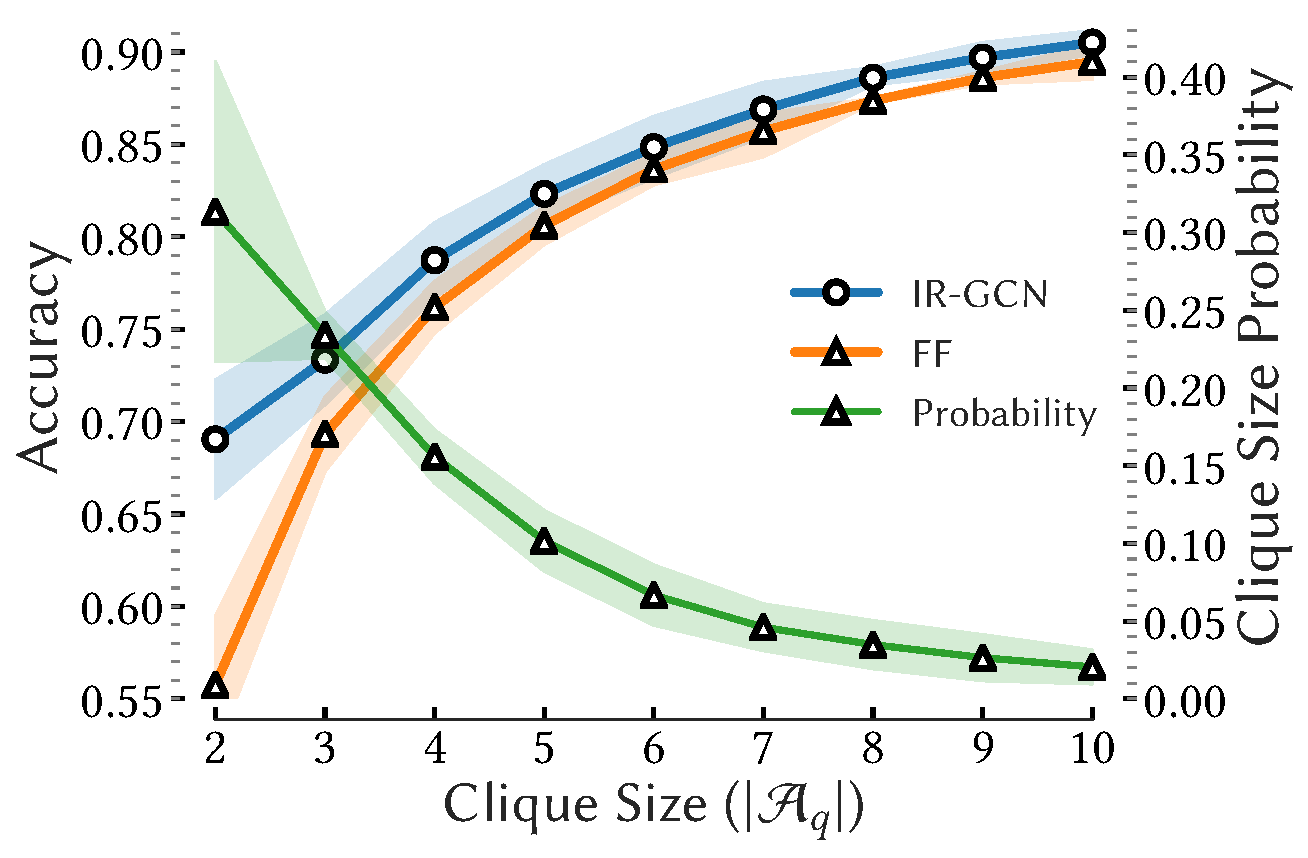
\includegraphics[scale=0.3]{figures/clique_acc.pdf}
%   %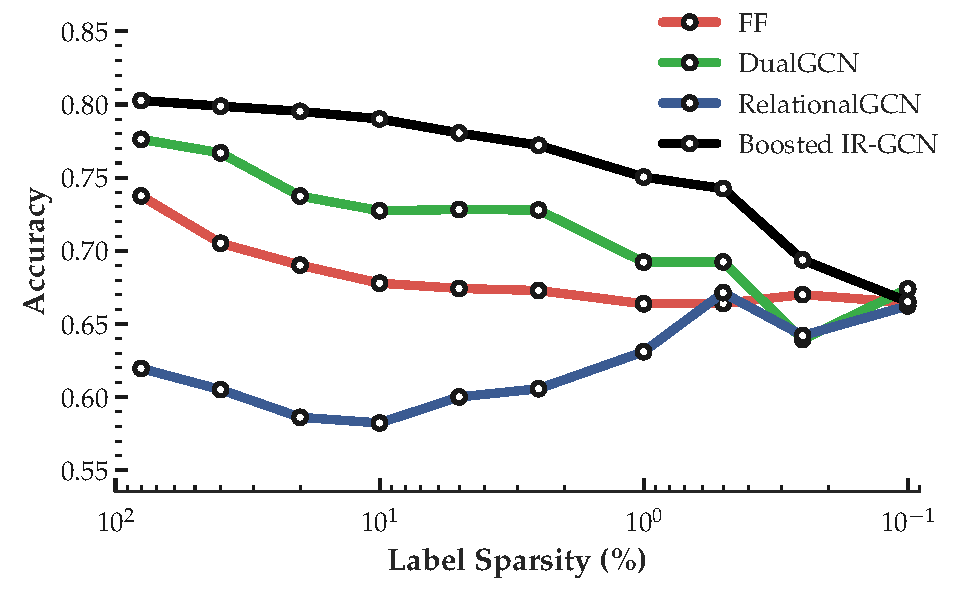
\includegraphics[height=4.2cm,width=0.85\linewidth]{figures/Label_Sparsity}
%   \vspace{-0.12in}
%   \caption{\small \label{fig:clique} Accuracy of our IR-GCN model compared to the FF model with varying clique size (i.e. number of answers to a question, $\vert \mathcal{A}_q \vert$) for Contrastive view . %The results are reported for the largest StackExchange community in all five categories.
% We report averaged results over the largest community of all categories. Our model performs much better for smaller cliques, and the effect diminishes for larger cliques (\cref{eq:contrast}). 80\% of the questions have $< 4$ answers.}
%   \vspace{-0.15in}
% \end{figure}

We show that due to our proposed modification to the convolution operation for contrastive view, we achieve \emph{Discriminative Magnification effect} (\cref{eq:contrast}). Note that the difference is scaled by Clique size ($1 + 1/n-1$), i.e. number of answers to a question, $\vert \mathcal{A}_q \vert$. Figure \ref{fig:clique} shows the accuracy of our IR-GCN model as compared to the FeedForward model with varying clique size. Recall that the FeedForward model predict node labels independent of other nodes and is not affected by clique size. We report average results over the same five communities as above. We can observe that increase in accuracy is much more for lower clique sizes (13\% improvement for $\vert \mathcal{A}_q \vert = 2$ and 4\% for $\vert \mathcal{A}_q \vert = 3$ on average). The results are almost similar for larger clique sizes. In other words, our model significantly outperforms the FeedForward model for questions with fewer candidate answers. However, around 80\% of the questions have very few answers($< 4$), and thus this gain over FF is significant.

\vspace{-0.2in}
\subsection{Label Sparsity}

\begin{figure}[tbh]
  \begin{subfigure}{0.4\textwidth}
    \centering
    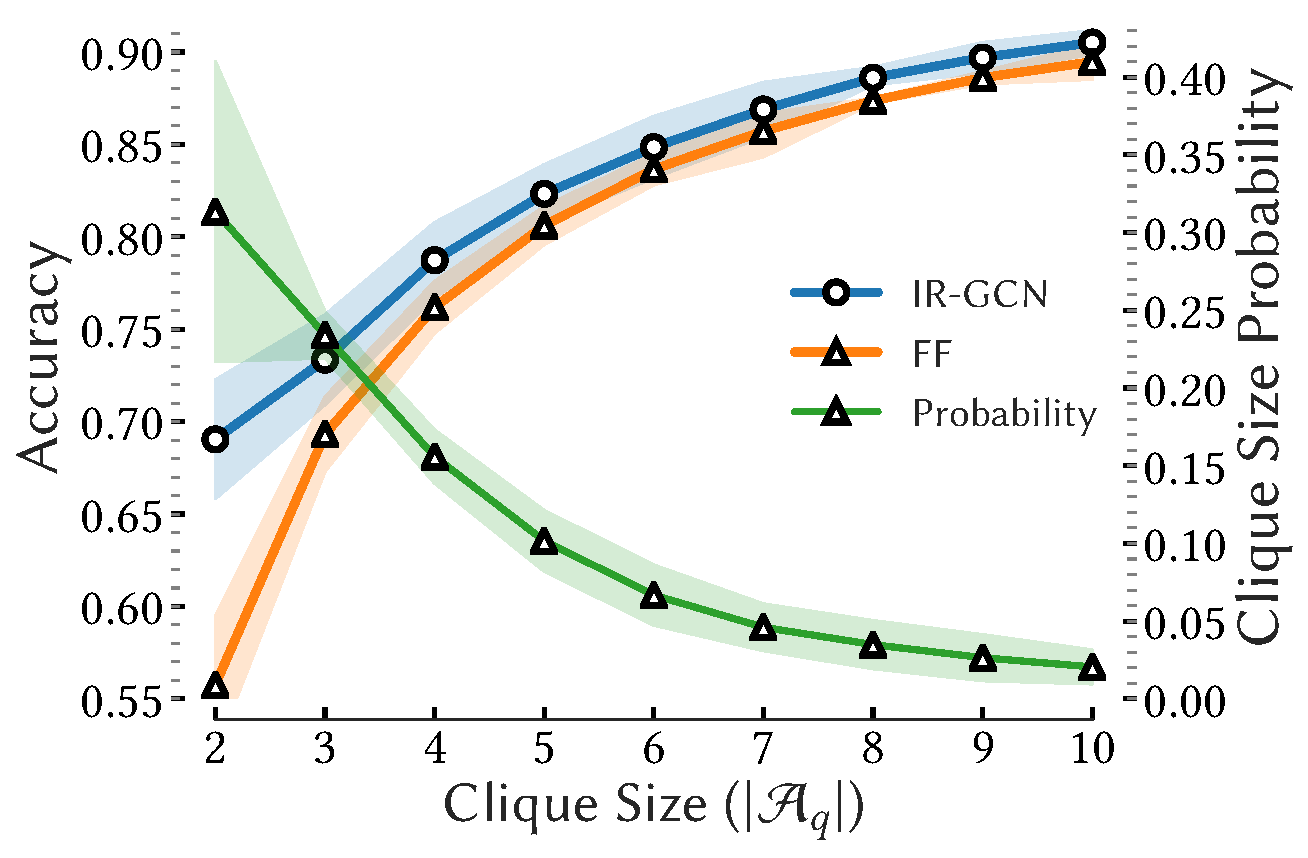
\includegraphics[scale=0.26]{figures/clique_acc.pdf}
    %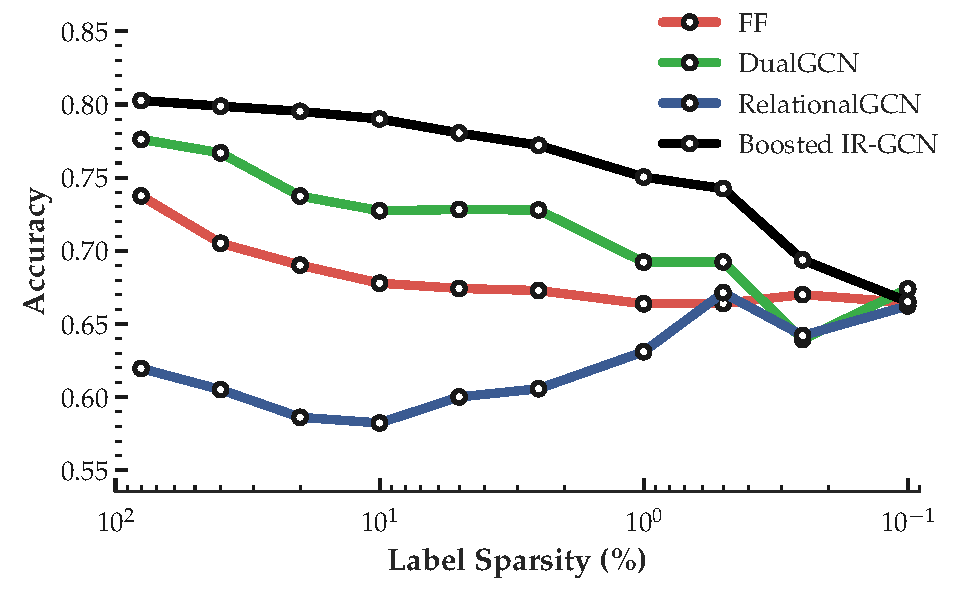
\includegraphics[height=4.2cm,width=0.85\linewidth]{figures/Label_Sparsity}
    \caption{\small \label{fig:clique}}
    %\vspace{-0.12in}
  \end{subfigure} \hspace{0.3in}
  \begin{subfigure}{0.55\textwidth}
      \centering
  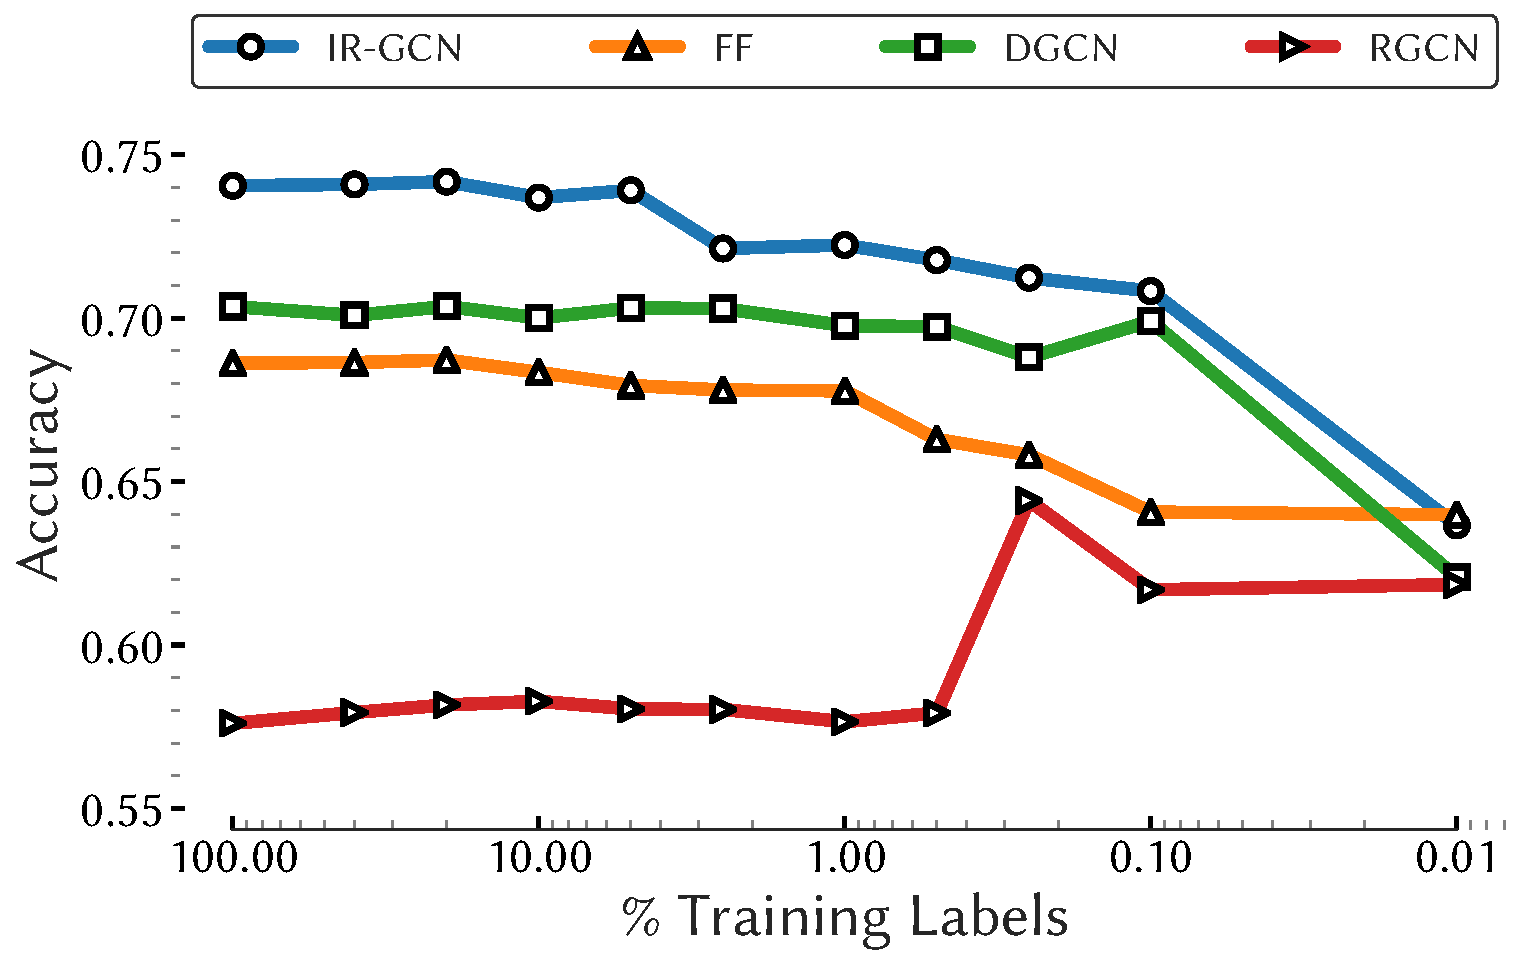
\includegraphics[scale=0.25]{figures/sparsity_acc_physics.pdf}
  %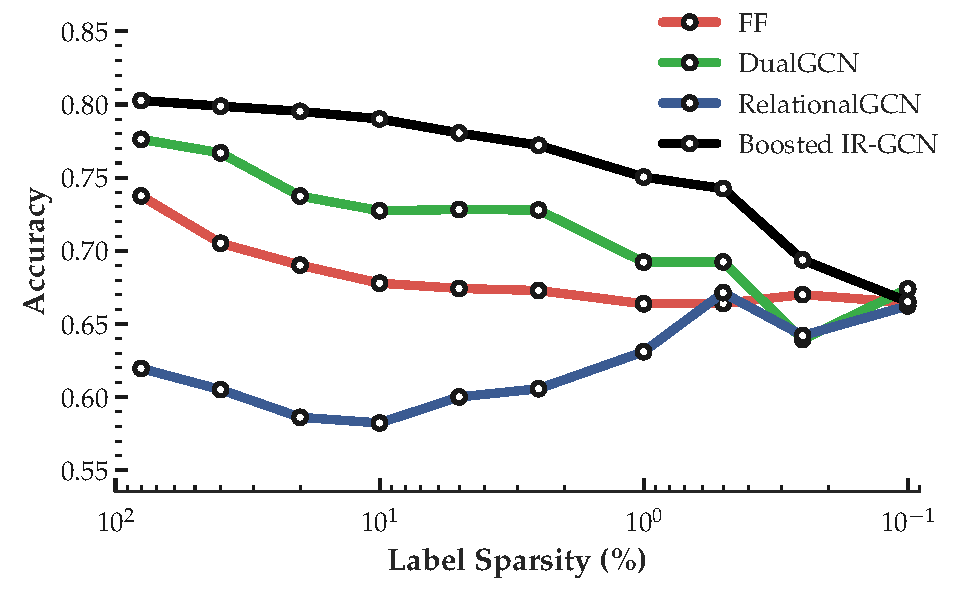
\includegraphics[height=4.2cm,width=0.85\linewidth]{figures/Label_Sparsity}
  %\vspace{-0.2in}
  \caption{\small\label{fig:labelsparsity} }
  \end{subfigure}
  %\vspace{-0.2in}
  \caption{\small a) Accuracy of our IR-GCN model compared to the FF model with varying clique size (i.e., number of answers to a question, $\vert \mathcal{A}_q \vert$) for Contrastive view. %The results are reported for the largest StackExchange community in all five categories.
We report averaged results over the largest community of all categories. Our model performs much better for smaller cliques, and the effect diminishes for larger cliques (\cref{eq:contrast}). 80\% of the questions have $< 4$ answers. \\
b) Change in accuracy with varying training label rates for Physics StackExchange. Our model is more robust to label sparsity than other relation ensemble approaches. RGCN works better with fewer labels as contrastive relation introduces noise in the model. At extreme sparsity, all approaches converge to the same value indicating random selection.
}
\end{figure}
Graph Convolution Networks are robust to label sparsity as they exploit graph structure and are thus heavily used for semi-supervised settings. Figure \ref{fig:labelsparsity} shows the change in accuracy for Physics StackExchange from the Science category at different training label rates. Even though our graph contains disconnected cliques, IR-GCN still preserves robustness to label sparsity.
In contrast, the accuracy of the FeedForward model declines sharply with less label information. Performance of DualGCN remains relatively stable while Relational GCN's performance increases with a decrease in label rate. Relational GCN assumes each view to be of similarity relation, and thus, adding contrastive relation introduces noise in the model. However, as the training labels become extremely sparse, the training noise decreases that leads to a marked improvement in the model. In the case of a meager label rate of 0.01\%, all approaches converge to the same value, which is the expectation of theoretically random selection. We obtained similar results for the other four StackExchange communities but omitted them for brevity.

% \subsection{Change in Accuracy with Clique Size}

\begin{comment}
\subsection{Contrastive GCN Analysis}
\label{ref:analysis}
The ability of neural networks to perform classification in sparse high-dimensional manifolds has been studied in past work, especially in the context of adversarial learning \cite{lu2017safetynet}. We employ the ReLU activation function in our convolution layers and study the outputs of the $k$th layer, i.e. embeddings with k-order locality. This transformation breaks the input space into cells with smooth gradients within each cell, at whose boundaries the piecewise linear function changes (i.e. the likelihood of the two classes of answers).

% In the context of adversarial learning \cite{safetynet} propose the existence of p-domains or cells in the learned manifold, representing a piecewise linear mapping of the transformed features to the class labels. The generalization neutrality property is particularly interesting. Both train and test samples are highly unlikely to lie in p-domains since the number of examples is much smaller than the capacity of the neural network to fit these regions. Weight decay can incentivize relatively small changes in the gradient across these regions resulting in smoother changes.  the ability of the network to fit such regions in the data manifold?

We ask a specific question in the context of our Contrastive IR-GCN. \emph{What is the impact of the layerwise discriminative magnification induced by our formulation?} Discriminative magnifications results in improved separability of the two classes in the later convolving layers, an effect we earlier demonstrated with a sample network in \cref{fig:contrast}. This positively impacts the ability of the model to explain the observed data points (i.e create p-domains that are well aligned with the contrastive samples provided) and improve the generalizability of the learned model to unseen data points. However, it is important to maintain sufficient regularization with weight decay to prevent sparse regions exhibiting sharp gradients which could affect model performance.

The capacity of our model can also be quantified in terms of the VC dimension of the aggregated classifier against the individual learners. Gradient boosting with multiple relation learners (each of which captures a specific aspect of node locality via graph convolution on the induced relations) could boost the capacity of the joint model, enabling better generalization and a more accurate fit in the data manifold (i.e. higher capacity to fit regions to fine distinctions).

Let us denote the upper bound of the VC dimension or capacity of each individual learner as D (If the individual learners do not have identical capacity, the minimum can be used to compute a lower bound on the aggregated learner capacity). Then the gradient boosted learner with T classifiers has a bound on it's capacity~\cite{shalev2014understanding} given by,
\begin{equation*}
\mathcal{VC}_{Agg}  = T \times (D+1) \times(3 \log(T.(D+1))+2)
\label{vcdim}
\vspace{-0.03in}
\end{equation*}

Thus we identify two potential reasons for our performance gains, first the discriminative magnification effect which also supports the strong individual performance of the contrast view, and second the gain in capacity from boosting, which could explain it's advantage over competing aggregation methods.

\end{comment}

%
% ---- Bibliography ----
%
% BibTeX users should specify bibliography style 'splncs04'.
% References will then be sorted and formatted in the correct style.
%
\small
\bibliographystyle{splncs04}
\bibliography{multiRelation-bib.bib}

\end{document}
